\documentclass[12pt]{report}


% Define margins
\setlength{\topmargin}{-1.0cm}
\setlength{\oddsidemargin}{0.1cm}
\setlength{\textwidth}{16.5cm}
\setlength{\textheight}{23.0cm}







% Define header and footer
\usepackage{lastpage}
\usepackage{fancyhdr}
\pagestyle{fancy}
\fancyhf{}
\lhead{{\includegraphics[height=.8cm]{figures/nus.png}}}
\rhead{\textbf{\textit{Interpretable and Fair Machine Learning}} }
\lfoot{\textbf{\textit{Page \thepage/\pageref*{LastPage}}}}
\renewcommand{\footrulewidth}{0.7pt}
\renewcommand{\headrulewidth}{0.7pt}



% Packages
\usepackage{amsmath}
\usepackage{amsthm,dsfont,amssymb}
\newtheorem{comment}{Comment}
%\theoremstyle{definition}
\usepackage[utf8]{inputenc} 
\usepackage{graphicx}
\usepackage{multirow}
\usepackage{color}
\usepackage{comment}
\usepackage{microtype}
\usepackage{wrapfig}
\usepackage{hyperref,url}
\usepackage[
font=footnotesize % or small or scriptsize
]{subfig}
\usepackage{booktabs}
\usepackage{caption}
\usepackage{enumitem,kantlipsum}
\usepackage{algorithm}
\usepackage[noend]{algpseudocode}


% Theorem
\newtheorem{theorem}{Theorem}
\newtheorem{definition}{Definition}
\newtheorem{axiom}{Axiom}
\newtheorem{property}[theorem]{Property}
\newtheorem*{remark}{Remark}
\newtheorem{lemma}[theorem]{Lemma}
\newtheorem{lemmarep}{Lemma}
\newtheorem{proposition}[theorem]{Proposition}
\newtheorem{example}{Example}[section]
\newtheorem{corollary}{Corollary}
\newtheorem{construction}[theorem]{Construction}



% Tikz
\usepackage{tikz}
\usetikzlibrary{automata}
\usetikzlibrary{bayesnet,arrows}
\usetikzlibrary{shapes,fit,calc,positioning}
\tikzset{box/.style={draw, diamond, thick, text centered, minimum height=0.5cm, minimum width=1cm, text width=0.9cm}}
\tikzset{line/.style={draw, thick, -latex'}}


% References
\usepackage{cite}
\usepackage[nameinlink,capitalize]{cleveref}  % easy referencing




% Macros
\newcommand{\red}[1]{\textcolor{red}{#1}}
\newcommand{\blue}[1]{\textcolor{blue}{#1}}
\newcommand{\green}[1]{\textcolor{green}{#1}}

% Fairness 
%	Justicia
			\newcommand{\justicia}{\ensuremath{\mathsf{Justicia}}}
			\newcommand{\nonsensitive}{\ensuremath{\mathbf{X}}}
			\newcommand{\sensitive}{\ensuremath{\mathbf{A}}}
			\newcommand{\bool}{\ensuremath{B}}
			\newcommand{\alg}{\mathcal{M}}
			\newcommand{\R}{\ensuremath{\raisebox{\depth}{\rotatebox{180}{R}}}}
			\newcommand{\justiciaenum}{\ensuremath{\mathsf{Justicia\_enum}}}
			\newcommand{\justicialearn}{\ensuremath{\mathsf{Justicia\_learn}}}
			\newcommand{\justiciacond}{\ensuremath{\mathsf{Justicia\_cond}}}
	
%	FVGM
			\newcommand{\fvgm}{\ensuremath{\mathsf{FVGM}}}
			\newcommand{\mediator}{\ensuremath{\mathbf{Z}}}
			\newcommand{\stochastic}{\ensuremath{\mathsf{S3P}}}
			\DeclareMathOperator*{\argmax}{arg\,max}
			\DeclareMathOperator*{\argmin}{arg\,min}
			\newcommand{\graph}{\ensuremath{G}}
			\newcommand{\factors}{\ensuremath{\theta}}
			\newcommand{\parent}{\ensuremath{\mathrm{Pa}}}
			\newcommand{\BN}{\ensuremath{\mathsf{BN}}}
			
%			color
			\definecolor{terminate}{gray}{0.8}
			\definecolor{collision}{rgb}{0.2,1,0.3}
			\definecolor{existential}{rgb}{0.9,0.9, 0.1}
			

% Interpretability
%		Relaxed CNF
			\newcommand{\Rule}{\ensuremath{{\mathcal{R}}}}
			\newcommand{\weight}[1]{\ensuremath{W \! \left( #1 \right)}}
			\newcommand{\X}{{\mathbf{X}}}
			\newcommand{\MaxSAT}{\ensuremath{\mathsf{MaxSAT}}}
			\newcommand{\noise}{\xi}
			\newcommand{\card}{\eta}
			\newcommand{\noclause}{k}
			\newcommand{\crr}{\ensuremath{\mathsf{CRR}}}
			\newcommand{\CNF}{\ensuremath{\mathsf{Card2CNF}}}
			\newcommand{\B}{\mathbf{b}}
			\newcommand{\clause}{\ensuremath{\mathsf{clause}}}
			\newcommand{\MLIC}{\ensuremath{\mathsf{MLIC}}}
			\newcommand{\IMLI}{\ensuremath{\mathsf{IMLI}}}
			\newcommand{\ILP}{\ensuremath{\mathsf{ILP}}}

			
			
			
			
			
			


\begin{document}
	\begin{center}
		\Large \textbf{Interpretable and Fair Machine Learning} \\
		\vspace{1em}
		\large Bishwamittra Ghosh
	\end{center}
	
	\section{Introduction}
The tremendous success of machine learning in recent years has found its applications in different high-stake and  safety-critical domains, such as medical, law, education, and transportation. In such domains, the interpretability and fairness of machine learning classifiers are of paramount importance. In this work, we focus on improving the interpretability and fairness in machine learning. 

There are two-fold objectives in interpretable machine learning: (i) designing classifiers that are interpretable by design and (ii) leveraging already interpretable models to explain the prediction of black-box classifiers. In this work, we propose an efficient learning framework~\cite{ghosh19incremental} for a rule-based classifier\textemdash a popular interpretable model because of expressing the decision function in terms of rules corresponding to input features.  Our framework allows us to learn classification rules expressible in propositional logic, for example, CNF (Conjunctive Normal Form) and DNF (Disjunctive formal form) formulas.  The benefit of learning CNF classifiers is that this is the fundamental block for learning other popular interpretable representations: decision lists and decision sets. Learning rule-based classifiers is an intractable problem because of solving a combinatorial optimization problem. To efficiently learn these classifiers, we propose a MaxSAT-based formulation and scale it by combining incremental learning. The result is an efficient learning framework that can classify datasets even with 1 million samples while also balancing between high accuracy and small rule size. As an application of incremental learning, we propose to learn more relaxed logical rules~\cite{ghosh20classification} which demonstrate higher succinctness in their representation while achieving better accuracy. Furthermore, as an application of MaxSAT, we solve group testing problems based on compressed sensing~\cite{ciampiconi20maxsat}. Our MaxSAT-based formulation for group testing has impressive scalability than state-of-the-art approaches. 



We study the application of interpretable machine learning models in explaining the prediction of black-box models such as neural networks. To this end, we propose a PAC-based (Probably Approximately Correct) local explanations of feed-forward and recurrent neural networks using rule-based classifiers and their variants~\cite{neider2020probably,ghosh2020formal}. To explain feed-forward neural networks, we learn flexible classification rules using SyGuS~\cite{neider2020probably}. Such rules have the theoretical property that they are PAC approximate to the neural network within the locality of a query of interest. Similarly, to explain recurrent neural networks, we propose learning explanations in LTL formulas (Linear Temporal Logic)~\cite{ghosh2020formal}. 


Machine learning models may become biased in their decisions towards certain demographic populations. One important question in fairness in machine learning is to verify whether the model is unfair or not with respect to multiple definitions of fairness studied in the literature. To this end, we propose a scalable fairness verification framework based on formal methods, particularly stochastic satisfiability (SSAT)~\cite{ghosh2020justicia} and stochastic subset-sum problem (S3P)~\cite{ghosh2021algorithmic}. The input to the fairness verifier is a machine learning model and the distribution of input features and the output is an assessment of different fairness metrics that the model obtains given the distribution. Our fairness verifier has the following advantages over existing verifiers. We can efficiently verify the fairness of compound sensitive groups\textemdash such as, white-male and black-female\textemdash by combining multiple sensitive features, unlike existing works that only consider a single binary sensitive feature. We also consider feature-correlation represented as a Bayesian network whereas existing methods consider limited correlation among features. As a result, the proposed verifier has higher accuracy than existing verifiers. Finally, our verifier is more scalable than existing verifiers because of the efficient formulation based on SSAT and S3P. 


As future work, we aim to combine the interpretability and fairness of machine learning in a single framework. In particular, we explain the unfairness of models by combining explanation methods in machine learning. Our hypothesis is that such a combination would be effective in identifying the bias of a model and also mitigate the bias through imperative actions.

	
	
	
%	Fairness
%		Justicia
			\chapter{Justicia: A Stochastic SAT Approach to Formally Verify Fairness}
				\section{Abstract}
	As a technology machine learning\improvement{Unnecessary abbreviation} is oblivious to societal good or bad, and thus, the field of fair machine learning has stepped up to propose multiple mathematical definitions and algorithms to ensure different notions of fairness in machine learning classifiers.	Given the multitude of propositions, it has become imperative to formally verify the fairness of different classifiers on different datasets.	In this chapter\change{Paper replaced with chapter}, we propose a \textit{stochastic satisfiability} (SSAT) based probabilistic fairness verification framework, called {\justicia}, that formally verifies different fairness measures of supervised classifiers given the distribution of input features. We instantiate {\justicia} on multiple classifiers, bias mitigation algorithms, and fairness datasets to verify different fairness metrics, such as disparate impact, statistical parity, and equalized odds.
	{\justicia} is scalable, accurate, and operates on non-Boolean and compound sensitive features\change{Attributes replaced with features} unlike existing probabilistic verifiers, such as FairSquare and VeriFair.
	Being distribution-based by design, {\justicia} is more robust than verifiers such as AIF360, that operate on specific test samples.
	We also theoretically bound the finite-sample error of the verified fairness measure.

				\section{Introduction}
%\paragraph{Motivation: ML + Fairness}
Machine learning (ML) is becoming the omnipresent technology of our time. 
ML algorithms are being used for high-stake decisions like college admissions, crime recidivism, insurance, and loan decisions.
Thus, human lives are now pervasively influenced by data, ML, and their inherent bias.

\begin{example}\label{fairness_justicia_example:intro}
Let us consider an example (Figure~\ref{fairness_justicia_fig:fair_example}) of deciding eligibility for health insurance depending on the fitness and income of the individuals of different age groups (20-40 and 40-60).
Typically, incomes of individuals increase as their ages increase while their fitness deteriorates.
We assume relation of income and fitness depends on the age as per the Normal distributions in Figure~\ref{fairness_justicia_fig:fair_example}.
Now, if we train a decision tree~\cite{narodytska2018learning} on these fitness and income indicators to decide the eligibility of an individual to get a health insurance, we observe that the `optimal' decision tree (ref. Figure~\ref{fairness_justicia_fig:fair_example}) selects a person above and below $40$ years with probabilities $0.18$ and $0.72$ respectively.
This simple example demonstrates that even if an ML algorithm does not explicitly learn to differentiate on the basis of a sensitive attribute, it discriminates different age groups due to the utilitarian sense of accuracy that it tries to optimize.
\end{example}

\begin{figure}[t!]
	\centering
	\begin{minipage}{.18\columnwidth}
		\centering
		\scalebox{0.5}{	
			\begin{tikzpicture}[x=1.5cm,y=1.8cm]
			% Define nodes
			\node[latent,scale=1.5] (a1) {$\textrm{age}$} ; %
			\node[obs, scale=1.5, below=of a1, xshift=-.6cm] (h) {$\textrm{fitness}$}; %
			\node[obs, scale=1.5, below=of a1, xshift=.6cm] (i) {$\textrm{income}$}; %
			\node[obs, scale=1.5, below=of h, xshift=.6cm] (p) {$\hat{Y}$}; %			
			%%add edge
			\edge[] {a1} {h,i} ;
			\edge[] {h,i} {p} ;
			\end{tikzpicture}
		}
	\end{minipage}\hfill
	\begin{minipage}{.2\columnwidth}
		\centering
		\includegraphics[scale=0.35]{figures/fairness/justicia/example.pdf}
	\end{minipage}\hfill
	\begin{minipage}{.5\columnwidth}
		\scalebox{0.37}{	
			\begin{tikzpicture}[x=1cm,y=1.8cm]
			\node [box, scale=2]                                    (p)      {fitness $\geq 0.61$};
			\node [scale=2, above= -0.1cm of p]  (a)    {Trained Decision Tree};
			\node [scale=2, box, below=  -1cm of p, xshift=-1.4cm]    (a1)    {income\\ $\geq 0.29$};
			\node [scale=2, box, below= -1cm of p, xshift=1.4cm]     (a2)    {income $\geq 0.69$};
			\node [scale=2,below= of a1, xshift=-1.2cm]  (a11)    { $1$};
			\node [scale=2,below= of a1, xshift=1.2cm]   (a12)    { $0 $};
			\node [scale=2,below= of a2, xshift=-1.2cm]  (a21)    { $1$};
			\node [scale=2,below= of a2, xshift=1.2cm]  (a22)    { $0$};
			%
			\path [line] (p) -|         (a1) node [scale=1.5,midway, above]  {Y};
			\path [line] (p) -|         (a2) node [scale=1.5,midway, above]  {N};
			\path [line] (a1) -|       (a11) node [scale=1.5,midway, above]  {Y};
			\path [line] (a1) -|       (a12) node [scale=1.5,midway, above]  {N};
			\path [line] (a2) -|       (a21) node [scale=1.5,midway, above]  {Y};
			\path [line] (a2) -|       (a22) node [scale=1.5,midway, above]  {N};
			\end{tikzpicture}}
	\end{minipage}%
	\caption{A trained decision tree to learn eligibility for health insurance using age-dependent fitness and income indicators.}\label{fairness_justicia_fig:fair_example}

\end{figure}
\subsubsection{Fair ML.} Statistical discriminations caused by ML algorithms have motivated researchers to develop several frameworks to ensure fairness and several algorithms to mitigate bias.
Existing fairness metrics mostly belong to three categories: \textit{independence}, \textit{separation}, and \textit{sufficiency}~\cite{mehrabi2019survey}. 
Independence metrics, such as demographic parity, statistical parity, and group parity, try and ensure the outcomes of an algorithm to be independent of the groups that the individuals belong to~\cite{feldman2015certifying,dwork2012fairness}.
Separation metrics, such as equalized odds, define an algorithm to be fair if the probability of getting the same outcomes for different groups are same~\cite{hardt2016equality}.
Sufficiency metrics, such as counterfactual fairness, constrain the probability of outcomes to be independent of individual's sensitive data given their identical non-sensitive data~\cite{kusner2017counterfactual}. %,wu2019counterfactual

In Figure~\ref{fairness_justicia_fig:fair_example}, independence is satisfied if the probability of getting insurance is same for both the age groups. Separation is satisfied if the number of `actually' (ground-truth) ineligible and eligible people getting the insurance are same. Sufficiency is satisfied if the eligibility is independent of their age given their attributes are the same.
Thus, we see that the metrics of fairness can be contradictory and complimentary depending on the application and the data~\cite{corbett2018measure}.
Different algorithms have also been devised to ensure one or multiple of the fairness definitions.
These algorithms try to rectify and mitigate the bias in the data and thus in the prediction-model in three ways: \textit{pre-processing} the data~\cite{kamiran2012data,zemel2013learning,calmon2017optimized}, \textit{in-processing} the algorithm~\cite{zhang2018mitigating}, and \textit{post-processing} the outcomes~\cite{kamiran2012decision,hardt2016equality}.

\subsubsection{Fairness Verifiers.} Due to the abundance of fairness metrics and difference in algorithms to achieve them, it has become necessary to verify different fairness metrics over datasets and algorithms. 

In order to verify fairness as a model property on a dataset, verifiers like \textit{FairSquare}~\cite{albarghouthi2017fairsquare} and \textit{VeriFair}~\cite{bastani2019probabilistic} have been proposed. 
%FairSquare verifies demographic parity and individual fairness as a numerical integration problem for a specific program semantics.
%VeriFair translates fairness metrics to an enumeration problem of a specified Boolean syntax.
%These papers operate for a specific Boolean sensitive attribute.
These verifiers are referred to as {\em distributional verifiers} owing to the fact that their inputs are a probability  distribution of the attributes in the dataset and a model of a suitable form, and their objective is to verify fairness w.r.t. the distribution and the model.
Though FairSquare and VeriFair are robust and have asymptotic convergence guarantees, we observe that they scale up poorly with the size of inputs and also do not generalize to non-Boolean and compound sensitive attributes.
In contrast to the distributional verifiers, another line of work, referred to as sample-based verifiers, has focused on the design of testing methodologies  on a given fixed data sample~\cite{galhotra2017fairness,aif360-oct-2018}. 
Since sample-based verifiers are dataset-specific, they generally do not provide robustness over the distribution.


%\blue{Other papers: Probabilistic Verification of Fairness Properties via	Concentration, Verifying Individual Fairness in Machine Learning Models~\cite{john2020verifying}}
Thus, a \textit{unified formal framework} to verify \textit{different fairness metrics} of an ML algorithm, which is \textit{scalable}, capable of \textit{handling compound protected groups}, \textit{robust} with respect to the test data, and \textit{operational on real-life} datasets and fairness-enhancing algorithms, is missing in the literature.

\subsubsection{Our Contribution.} From this vantage point, \textit{we propose to model verifying different fairness metrics as a Stochastic Boolean Satisfiability (SSAT) problem}~\cite{littman2001stochastic}.
SSAT was originally introduced by ~\cite{papadimitriou1985games} to model {\em games against nature}. In this work, we primarily focus on reductions to the exist-random quantified fragment of SSAT, which is also known as E-MAJSAT~\cite{littman2001stochastic}. 
SSAT is a conceptual framework that has been employed to capture several fundamental problems in AI such as computation of maximum a posteriori (MAP) hypothesis~\cite{fremont2017maximum},  propositional probabilistic planning~\cite{majercik2007appssat},  and circuit verification~\cite{lee2018towards}.
Furthermore, our choice of SSAT as a target formulation is motivated by the recent algorithmic progress that has yielded efficient SSAT tools~\cite{lee2017solving,lee2018solving}.



%We formulate SSAT encodings of the fairness verification problems and two methods to evaluate them in order to verify independence and separation metrics for any supervised learning algorithm using a unified scheme.
%Our encodings not only allow us to compute for non-Boolean and compound sensitive attributes but also to scale significantly better than existing formal verifiers. 
%We perform experimental analysis for multiple fairness metrics, datasets, and algorithms to instantiate the efficiency and effectiveness of our approach.

Our contributions are summarised below:
\begin{itemize}
	\item We propose a unified SSAT-based approach, {\justicia}, to verify independence and separation metrics of fairness for different datasets and classification algorithms.
	%\item \blue{{\justicia} measures fairness metrics for pre-, in-, and post-processing algorithms with respect to the data  generating distribution}.
	\item Unlike previously proposed formal distributional verifiers, namely FairSquare and VeriFair, {\justicia} verifies fairness for compound and non-Boolean sensitive attributes.%, and also \red{separation metrics}.
	\item Our experiments validate that our method is more accurate and scalable than the distributional verifiers, such as FairSquare and VeriFair, and more robust than the sample-based empirical verifiers, such as AIF360.
	\item We prove a finite-sample error bound on our estimated fairness metrics which is stronger than the existing asymptotic guarantees.
\end{itemize}

It is worth remarking that significant advances in AI bear testimony to the right choice of formulation, for example, formulation of planning as SAT~\cite{kautz1992planning}. In this context, we view that formulation of fairness as SSAT has potential to spur future work from both the modeling and encoding perspective as well as core algorithmic improvements in the underlying SSAT solvers.  

\iffalse
With this growing set of algorithms and definitions, it has become important to measure and verify fairness and bias of different algorithms and datasets. 
One popular approach is to use specific test dataset to compute the related statistical quantities and to certify fairness for that specific test dataset.
AIF360~\cite{aif360-oct-2018} provides a unified framework to implement multiple algorithms and to measure their fairness depending on such test datasets.
Though this method of verification works for a specified datasets, such verifiers do not explain how much a fairness measure depends on which sensitive attribute and is not robust to the selection of test dataset and its size.
\fi
				\section{Background: Fairness and SSAT}
\label{fairness_justicia_sec:preliminaries}

In this section, we define different fairness metrics for a supervised learning problem. Following that, we discuss Stochastic Boolean Satisfiability (SSAT) problem.

\subsection{Fairness Metrics for Machine Learning}\label{fairness_justicia_sec:fairness}


We consider\footnote{{We represent sets/vectors by bold letters, and the corresponding distributions by calligraphic letters. We express random variables in uppercase, and an assignment of a random variable in lowercase.}} a dataset $ \mathbf{D} $ as a collection of triples $ (\nonsensitive, \sensitive, Y) $ generated from an underlying distribution $\mathcal{D}$. $ \nonsensitive \triangleq \{X_1, \dots, X_{\numnonsensitive}\} $ are non-sensitive features whereas $ \sensitive \triangleq \{A_1, \dots, A_{\numsensitive}\} $ are categorical sensitive features.  $Y \in \{0,1\}$ is the binary label (or class) of $(\nonsensitive,\sensitive)$. Each non-sensitive feature $ X_i$ is sampled from a continuous probability distribution {$ \mathcal{X}_i $}, and each sensitive feature $ A_j \in \{0, \dots, N_j\}  $ is sampled from a discrete probability distribution {$ \mathcal{A}_j $}. We use $ (\mathbf{x}, \mathbf{a}) $ to denote the feature-values of  $ (\nonsensitive, \sensitive) $.  For sensitive features, a valuation vector $ \mathbf{a} = [a_1, .., a_{\numsensitive}] $ is called a \textit{compound sensitive group}. For example, consider $ \sensitive = $ \{race, sex\} where race $ \in $ \{Asian, Color, White\} and sex $ \in $ \{female, male\}. Thus $ \mathbf{a} = $ [Asian, female]  is a compound sensitive group. 
We represent a binary classifier trained on the dataset $\mathbf{D}$ as $\alg: (\nonsensitive, \sensitive) \rightarrow \hat{Y} $. Here, $\hat{Y} \in \{0,1\}$ is the predicted class of $ (\nonsensitive, \sensitive) $.



As we illustrated in Example~\ref{fairness_justicia_example:intro}, a classifier $\alg$ that solely optimizes accuracy, i.e., the average number of times $\hat{Y} = Y$, may discriminate certain compound sensitive groups over others~\cite{chouldechova2020snapshot}. In the following, we describe two well-known fairness definitions verified by {\justicia}: group fairness and causal fairness. To this end, we use $ f(\alg, \mathcal{D}) $ to quantify the fairness of the classifier $ \alg $ provided the distribution of features $ \mathcal{D} $. More specifically,  {\justicia} verifies fairness metrics where $ f(\alg, \mathcal{D}) $ depends on the conditional Positive Predictive Value (PPV) of the classifier, denoted by $ \Pr[\hat{Y} = 1 | \mathsf{C}] $. Henceforth, each fairness metric is identified by the particular choice of the conditional $ \mathsf{C} $, as discussed next.

\subsubsection{Group Fairness.} Group fairness is categorized into three families: independence, separation and sufficiency, of which {\justicia} verifies independence and separation metrics. 
The independence metrics state that the predicition of the classifier should be independent of compound sensitive groups. Formally, independence notion specifies an equal PPV across all sensitive groups for a classifier, i.e., $\Pr[\hat{Y} =1 | \mathbf{A} =  \mathbf{a}]  =  \Pr[\hat{Y} =1 | \mathbf{A} =  \mathbf{a}'] , \forall \mathbf{a}, \mathbf{a}' \in \sensitive$.
Since satisfying independence exactly is hard, relaxations of independence fairness metrics, such as \textit{disparate impact} and \textit{statistical parity}, are proposed in the literature~\cite{dwork2012fairness,feldman2015certifying}.

\textit{Disparate impact} (DI) measures the ratio of PPVs between the most favored group and least favored group, and prescribe it to be close to $1$~\cite{feldman2015certifying}.  Formally, the disparate impact of a classifier is 
\[
f_{\mathsf{DI}}(\alg, \mathcal{D}) \triangleq \frac{\min_{\mathbf{a}} \Pr[\hat{Y} =1 | \mathbf{A} =  \mathbf{a}]}{\max_{\mathbf{a}} \Pr[\hat{Y} =1 | \mathbf{A} =  \mathbf{a}]},
\]
where the subscript of $ f $ denotes the corresponding fairness metric.

Another popular relaxation of independence metrics  is \textit{statistical parity} (SP) that measures the maximum difference of PPVs among sensitive groups, and prescribe this quantity to be near zero. Thus, the statistical parity of  a classifier is 
\[ f_{\mathsf{SP}}(\alg, \mathcal{D}) \triangleq \max_{\mathbf{a}}\Pr[\hat{Y} =1 | \mathbf{A} = \mathbf{a}] - \min_{\mathbf{a}}\Pr[\hat{Y} =1 | \mathbf{A} = \mathbf{a}]. \]



In the \textit{separation (or classification parity)} notion of fairness, the predicted label $\hat{Y}$ of a classifier is independent of the sensitive features $\sensitive$ given the class labels $Y$. In case of binary classifiers, a popular separation metric is \textit{equalized odds} (EO)~\cite{hardt2016equality} that computes the maximum difference of false positive rates \red{(FPR)} and true positive rates \red{(TPR)} conditioned on sensitive groups. Formally,  for $ Y \in \{0,1\} $,  the equalized odds of a classifier is defined as 
\begin{align*}
f_{\mathsf{EO}}(\alg, \mathcal{D})  \triangleq \max(&\max_{\mathbf{a}}\Pr[\hat{Y} =1 | \mathbf{A} = \mathbf{a}, Y = 0] - \min_{\mathbf{a}}\Pr[\hat{Y} =1 | \mathbf{A} = \mathbf{a}, Y = 0], \\
&\max_{\mathbf{a}}\Pr[\hat{Y} =1 | \mathbf{A} = \mathbf{a}, Y = 1] - \min_{\mathbf{a}}\Pr[\hat{Y} =1 | \mathbf{A} = \mathbf{a}, Y = 1]). 
\end{align*}


\subsubsection{Path-specific Causal Fairness.}
Let $ \mathbf{a}_{\max}  \triangleq \argmax_{ \mathbf{a}} \Pr[\hat{Y} =1 |\mathbf{A}=  \mathbf{a}] $. We consider mediator features $ \mediator \subseteq \nonsensitive $ sampled from the conditional distribution $ {\mathcal{Z}_{|\mathbf{A} = \mathbf{a}_{\max}}} $. This emulates the fact that mediator variables have the same sensitive features $ \mathbf{a}_{\max} $.   To this end, the path-specific causal fairness of a classifier is \[
 f_{\mathsf{PCF}}(\alg, \mathcal{D}) \triangleq \max_{\mathbf{a}}\Pr[\hat{Y} = 1 | \sensitive =  \mathbf{a}, \mediator] - \min_{\mathbf{a}} \Pr[\hat{Y} = 1 | \sensitive = \mathbf{a}, \mediator ].
\]



Therefore, PCF constrains that $ \hat{Y} $ is not directly dependent of $ \sensitive $ while $ \sensitive $ may indirectly affects $ \hat{Y} $ only through $ \mediator $. PCF is a variation of counterfactual fairness and causal fairness without mediator features~\cite{bastani2019probabilistic}. 




\begin{example}
	Following~\cite{bastani2019probabilistic}, we consider a classifier that decides the hiring of employees based on three features: gender (sensitive), years of experience (non-sensitive), and college-participation (mediator). It is practical to consider that gender $ \in $ \{male, female\} can affect the college-participation of individuals, and all three features are determining factors for the hiring process. Let `male' be the most favored group by the classifier, for instance. Path-specific causal fairness (PCF) ensures that a female candidate should be given a job offer with similar probability as a male candidate (by constraining $ \epsilon \approx 0 $). She,  however,  went to (participated in) college as if she were a male candidate while other non-mediator features such as  `years of experience' are the same.  Therefore, PCF measures the effect of gender on job offer, but ignores the effect of gender on whether candidates went to college.
\end{example}	



\paragraph{Fairness Certification.} We certify the fairness of a classifier by comparing $ f(\alg, \mathcal{D}) $ with a fairness threshold, denoted by $ \epsilon \in [0,1] $, which quantifies the desired level of fairness. In particular, a classifier is $ \epsilon $-fair with respect to statistical parity, equalized odds, or path-specific causal fairness if and only if $ f(\alg, \mathcal{D}) \le \epsilon $. In contrast, a classifier satisfies $(1 - \epsilon)$-disparate impact  if and only if $ f(\alg, \mathcal{D}) \ge 1 - \epsilon $. In all above fairness metrics, a lower value of $ \epsilon $ refers to higher fairness of the classifier.






\subsection{Stochastic Boolean Satisfiability (SSAT)}\label{fairness_justicia_sec:ssat}
Let $\mathbf{B}  = \{\bool_1, \dots, \bool_m\}  $ be a set of Boolean variables. A \textit{literal} is a variable $ \bool_i $ or its complement $ \neg \bool_i $. 
A propositional formula $\phi$ defined over $\mathbf{B}$ is in \textit{Conjunctive Normal Form (CNF)} if $\phi$   is  a conjunction of clauses and each clause is a disjunction of literals. 
%\red{DNF (disjunctive normal form) is the  complement of CNF where  the formula is a disjunction of clauses and each clause is  a conjunction of literals.} 
Let $ \sigma $ be an assignment to the  variables $ \bool_i \in \mathbf{B} $  such that $ \sigma(\bool_i) \in \{1, 0\} $. The propositional  \textit{satisfiability} problem (SAT) finds an assignment $ \sigma $ to all $ \bool_i \in  \mathbf{B} $ such that the formula $ \phi $ is evaluated to be $1$ (equivalently, true). 
In contrast to the SAT problem, the \textit{Stochastic Boolean Satisfiability} (SSAT) problem~\cite{littman2001stochastic} is computes the  probability of the satisfaction of the formula $\phi$ defined on \textit{quantified} Boolean variables. 
An SSAT formula is of the form
\begin{equation}\label{fairness_justicia_eq:ssat}
\Phi = Q_1\bool_1, \dots, Q_m \bool_m,\; \phi, 
\end{equation}
where $ Q_i \in \{\exists, \forall, \R^{p_i}\} $ is either of the existential ($\exists$), universal ($\forall$), or randomized ($\R^{p_i}$) quantifiers on $\bool_i$ and $\phi$ is a quantifier-free CNF formula. In case of a randomized quantifier $ \R^{p_i} $, $ p_i \in [0,1] $ is the probability of $ \bool_i $ being assigned to $ 1 $. In the SSAT formula $ \Phi $, the quantifier part $ Q_1\bool_1, \dots, Q_m \bool_m $ is known as the \textit{prefix} of the formula $ \phi $.  Let $ \bool $ be the outermost variable in the prefix. The semantics of SSAT formulas are defined recursively in the following.
\begin{enumerate}
	\item $ \Pr[\text{true}] = 1 $,  $ \Pr[\text{false}] = 0 $, 
	\item $ \Pr [\Phi] = \max_{\bool} \{\Pr[\Phi|_{\bool}], \Pr[\Phi|_{\neg \bool}]\}$ if $ \bool $ is existentially quantified ($ \exists $), 
	\item $ \Pr [\Phi] = \min_{\bool} \{\Pr[\Phi|_{\bool}], \Pr[\Phi|_{\neg \bool}]\} $ if $ \bool $ is universally quantified ($ \forall $), 
	\item $ \Pr [\Phi] = p\Pr[\Phi|_{\bool}] + (1-p) \Pr[\Phi|_{\neg \bool}] $ if $ \bool $ is randomized quantified ($\R^{p}$) with probability $p$ of being $\text{true}$,
\end{enumerate}
where $ \Phi|_{\bool} $ and $ \Phi|_{\neg \bool} $ denote the SSAT formulas derived by eliminating the outermost quantifier of $ \bool $  by substituting the value of $ \bool $ in the formula $ \phi $ with $ 1 $ and $ 0 $, respectively. In this paper, we focus on two specific types of SSAT formulas:  \textit{random-exist} (RE) SSAT and \textit{exist-random} (ER) SSAT. In the ER-SSAT (resp.\ RE-SSAT) formula, all existentially (resp.\ randomized) quantified variables are followed by randomized (resp.\ existentially) quantified variables in the prefix.


\begin{remark}
	ER-SSAT problem is $\mathrm{NP}^{\mathrm{PP}}$-hard whereas RE-SSAT problem is $\mathrm{PP}^{\mathrm{NP}}$-complete~\cite{littman2001stochastic}.
\end{remark}



The problem of SSAT and its variants have been pursued by theoreticians and practitioners for over three decades~\cite{majercik2005dc,fremont2017maximum,huang2006combining}. We refer the reader to~\cite{lee2017solving,lee2018solving} for detailed survey. It is worth remarking that the past decade has witnessed a significant performance improvements of SSAT solving, thanks to the close integration of techniques from SAT solving with advances in weighted model counting~\cite{sang2004combining,chakraborty2013scalable,chakraborty2014distribution}. 




				\section{{\justicia}: An SSAT Framework to Verify Fairness Metrics}
\label{fairness_justicia_sec:framework}
In this section, we present the primary contribution of this paper, {\justicia}, which is an SSAT-based framework for verifying independence and separation metrics of fairness. 

Given a binary classifier $\alg$ and a probability distribution over dataset $(X,A,Y) \sim \mathcal{D} $, our goal is to verify whether $\alg$ achieves independence and separation metrics with respect to the distribution $\mathcal{D}$. We  focus on a classifier that can be translated to a CNF formula of Boolean variables $\mathbf{B} $. 
The probability $ p_i $ of $\bool_i \in \mathbf{B}$ being assigned to $1$ is induced by the data generating distribution $\mathcal{D}$. 
In order to verify fairness metrics in compound protected groups, we discuss an enumeration-based approach and an equivalent learning-based approach. 
%We conclude this section by proposing a conditional distribution based enumeration for compound protected groups in Section~\ref{fairness_justicia_sec:cond_ssat}. 
We then provide a theoretical analysis for a high-probability error bound on the fairness metric and conclude with extension of {\justicia} in practical settings.

\iffalse
In this section, we present the main contribution of this paper, {\justicia}, which is an SSAT framework for verifying independence and separation metrics of fairness. 
We first state the problem formally in Section~\ref{fairness_justicia_sec:problem_statement}. 
To verify fairness metrics in compound protected groups, we discuss an enumeration approach in Section~\ref{fairness_justicia_sec:enumeration_ssat} and an equivalent but more efficient learning approach in Section~\ref{fairness_justicia_sec:learn_ssat}. 
We conclude this section by proposing a conditional distribution based enumeration for compound protected groups in Section~\ref{fairness_justicia_sec:cond_ssat}. 


\subsection{Problem Statement}
\label{fairness_justicia_sec:problem_statement}
Given a binary classifier $\alg$ and a probability distribution over dataset $(X,A,Y) \sim \mathcal{D} $, our goal is to verify whether $\alg$ achieves independence and separation metrics with respect to the distribution $\mathcal{D}$. We  focus on a classifier that can be translated to a CNF formula of Boolean variables $\mathbf{B} $. 
The probability $ p_i $ of $\bool_i \in \mathbf{B}$ being assigned to $1$ is induced by the data generating distribution $\mathcal{D}$. 
In our contribution, we reduce the verification problem to solving appropriately designed SSAT instances.
\fi 

\subsection{Evaluating Fairness with RE-SSAT Encoding}
\label{fairness_justicia_sec:enumeration_ssat}
In order to verify independence and separation metrics, the core component of {\justicia} is to compute the positive predictive value $\Pr[\hat{Y} = 1 | A = \mathbf{a}]$ for a compound protected group $\mathbf{a}$.  For simplicity, we  initially make some assumptions and discuss their practical relaxations later in this section.   
We first assume the classifier $\alg$ is representable as a CNF formula, namely $\phi_{\hat{Y}}$, such that $ \hat{Y} = 1 $ when $ \phi_{\hat{Y}}$ is satisfied and  $\hat{Y} =0$ otherwise. Since a Boolean CNF classifier is defined over Boolean variables, we  assume all attributes in $X$ and $A$ to be Boolean. Finally, we assume independence of non-protected attributes on protected attributes and $p_i $ is the  probability of the attribute $ \nonsensitive_i $ being assigned to $ 1 $ for any  $\nonsensitive_i \in X  $. 

Now, we define an RE-SSAT formula $\Phi_{\mathbf{a}}$ to compute the probability $\Pr[\hat{Y} = 1 | A = \mathbf{a}]$. In the prefix of $ \Phi_{\mathbf{a}} $,  all non-protected Boolean attributes in $X$ are assigned randomized quantification and they are followed by the protected Boolean attributes in $ A $ with existential quantification. The CNF formula $ \phi $ in $ \Phi_{\mathbf{a}} $ is constructed such that $ \phi $ encodes the event inside the target probability $ \Pr[\hat{Y} = 1 | A = \mathbf{a}] $. In order to encode the conditional $ A = \mathbf{a} $, we take the conjunction of the Boolean variables in $ A $ that symbolically specifies the compound protected group $ \mathbf{a} $. For example, we represent two protected attributes: race $ \in $ \{White, Colour\} and sex $ \in $ \{male, female\} by the Boolean variables $ R $ and $ S $  respectively. Hence, the compound groups $\{\textrm{White}, \textrm{male}\}$ and $\{\textrm{Colour}, \textrm{female}\}$ are represented by $ R \wedge S $ and $ \neg R \wedge \neg S $, respectively. Thus, the RE-SSAT formula for computing the probability  $ \Pr[\hat{Y} = 1 | A = \mathbf{a}] $ is
\begin{equation}	\label{fairness_justicia_eq:re}
\begin{split}
	\Phi_{\mathbf{a}} := \underbrace{\R^{p_{1}}\nonsensitive_1, \dots, \R^{p_{m}}\nonsensitive_m}_{\text{non-protected attributes}},  &\underbrace{\exists \sensitive_1,\dots, \exists \sensitive_n}_{\text{protected attributes}},
\phi_{\hat{Y}} \wedge (A=\mathbf{a}).\notag
\end{split}
\end{equation}
In $ \Phi_{\mathbf{a}} $, the existentially quantified variables $ \sensitive_1, \dots, \sensitive_n $ are assigned values  according  to the constraint $ A=\mathbf{a} $. \footnote{An RE-SSAT formula becomes an R-SSAT formula when the assignment to the existential variables are fixed.} Therefore, by solving the SSAT formula $ \Phi_{\mathbf{a}} $,  the SSAT solver finds the probability $ \Pr[\Phi_{\mathbf{a}}] $ for the protected group $ A=\mathbf{a} $ given the random values of $ \nonsensitive_1, \dots, \nonsensitive_m $, which is the PPV of the protected group $\mathbf{a} $ for the distribution $ \mathcal{D} $ and algorithm $\alg$. 

For simplicity, we have described computing the PPV of each compound protected group without considering the correlation between the protected and non-protected attributes. In reality, correlation exists between the protected and non-protected attributes. Thus, the non-protected attributes may have different conditional distributions for different protected groups. We incorporate these conditional distributions in RE-SSAT encoding by evaluating the conditional probability $ p_i = \Pr[\nonsensitive_i =\text{TRUE}| A=\mathbf{a}] $ instead of the independent probability $\Pr[\nonsensitive_i =\text{TRUE}]$ for any $\nonsensitive_i\in \nonsensitive$. We illustrate this method in Example~\ref{fairness_justicia_example:re_ssat}.
%This relaxes the independence requirement.

\begin{example}[RE-SSAT encoding]
	\label{fairness_justicia_example:re_ssat}
	Here, we illustrate the RE-SSAT formula for calculating the PPV for the protected group `age $ \ge 40 $' in the decision tree of Figure~\ref{fairness_justicia_fig:fair_example}. We assign three Boolean variables $ F,I,J $ for the three nodes in the tree such that the literal $ F,I,J $ denote `fitness $ \ge 0.61 $', `income $ \ge 0.29 $', and `income $ \ge 0.69 $', respectively. We consider another Boolean variable $A$  where the literal $ A $ represents the protected group `age $ \ge 40 $'. Thus, the CNF formula  for the decision tree is $ (\neg F \vee I) \wedge (F \vee J) $. From the distribution in Figure~\ref{fairness_justicia_fig:fair_example}, we get $ \Pr[F] = 0.41, \Pr[I] = 0.93 $, and $ \Pr[J] = 0.09 $. Given this information, we calculate the PPV for the protected group `age $ \ge 40 $' by solving the RE-SSAT formula:
	\begin{equation}
	\Phi_A := \R^{0.41}F, \R^{0.93}I, \R^{0.09}J, \exists A, \; (\neg F \vee I) \wedge (F \vee J) \wedge A.\notag
	\end{equation}
	From the solution to this SSAT formula, we get $ \Pr[\Phi_A] = 0.43 $. Similarly, to calculate the PPV for the group `age $ < 40 $', we replace the unit (single-literal) clause $ A $ with $ \neg A $ in the CNF in $ \Phi_A $ and construct another SSAT formula $ \Phi_{\neg A} $ where $ \Pr[\Phi_{\neg A}] = 0.43 $. 
	Therefore, if $\Pr[F], \Pr[I], \Pr[J]$ are computed independently of $A$ and $\neg A$, both age groups demonstrate equal PPV as the protected attribute is not explicitly present in the classifier. 
	However, there is an implicit bias in the data distribution for different protected groups and the classifier unintentionally learns it. 
	To capture this implicit bias, we calculate the conditional probabilities  $ \Pr[F|A] = 0.01, \Pr[I|A] = 0.99 $, and $ \Pr[J|A] = 0.18 $ from the distribution. Using the conditional probabilities in  $\Phi_A $, we find that $ \Pr[\Phi_A] = 0.18 $ for `age $ \ge 40 $'. For `age $ < 40 $',  we similarly obtain $ \Pr[F|\neg A] = 0.82, \Pr[I|\neg A] = 0.88 $, and $ \Pr[J|\neg A] = 0.01 $, and thus  $ \Pr[\Phi_{\neg A}] = 0.72 $. 
	Therefore, presented RE-SSAT encoding detects the discrimination of the classifier among different protected groups. An astute reader would observe that $I$ and $J$ are not independent. Following~\cite{chavira2008probabilistic}, we can simply capture relationship between the variables using constraints and if needed, auxiliary variables. In this case, it suffices to add the the constraint $J \rightarrow I$. 
\end{example}

\subsubsection{Measuring Fairness Metrics.}
As we compute the probability $\Pr[\hat{Y} = 1 | A = \mathbf{a}]$ by solving the SSAT formula $ \Phi_\mathbf{a} $, we  use $ \Pr[\Phi_\mathbf{a}] $ to measure different fairness metrics. 
For that, we compute $ \Pr[\Phi_\mathbf{a}] $ for all compound groups $\mathbf{a} \in A$ that requires solving exponential (with $n$) number of SSAT instances. 
We elaborate this enumeration approach, namely {\justiciaenum}, in Algorithm~\ref{fairness_justicia_algo:enum}  (Line~\ref{fairness_justicia_algo:justicia_enum_begin}--\ref{fairness_justicia_algo:justicia_enum_end}).

\begin{algorithm}[t!]
	\caption{\justicia: SSAT-based Fairness Verifier}
	\label{fairness_justicia_algo:enum}
	\footnotesize
	\begin{algorithmic}[1]
		\Function{{\justiciaenum}}{$ X,A,\hat{Y} $}
		\label{fairness_justicia_algo:justicia_enum_begin}
		\State $ \phi_{\hat{Y}} := \mathsf{CNF}(\hat{Y} = 1) $
		%\State $ p_{i} = \mathsf{CalculateProb}(\nonsensitive_i), \forall \nonsensitive_i \in X $
		\ForAll{$\mathbf{a} \in A$ }
		\State $ p_{i} \leftarrow \mathsf{CalculateProb}(\nonsensitive_i | \mathbf{a}), \forall \nonsensitive_i \in X $
		\State $ \phi := \phi_{\hat{Y}} \wedge (A=\mathbf{a}) $
		\State $  \Phi_\mathbf{a} := \R^{p_{1}}\nonsensitive_1, \dots, \R^{p_{m}}\nonsensitive_m, \exists \sensitive_1,\dots, \exists \sensitive_n,  \phi $
		\State $ \Pr[\Phi_\mathbf{a}]  \leftarrow \mathsf{SSAT}(\Phi_\mathbf{a}) $ \Comment{returns a probability}
		\EndFor
		\State \Return $ \max_{\mathbf{a}} \; \Pr[\Phi_{\mathbf{a}}], \min_{\mathbf{a}} \; \Pr[\Phi_{\mathbf{a}}] $
		\label{fairness_justicia_algo:justicia_enum_end}
		\EndFunction
		
		
		
		\Function{{\justicialearn}}{$ X,A,\hat{Y} $}
		\label{fairness_justicia_algo:justicia_learn_begin}
		\State $ \phi_{\hat{Y}} := \mathsf{CNF}(\hat{Y}  = 1) $
		\State $ p_{i} \leftarrow \mathsf{CalculateProb}(\nonsensitive_i), \forall \nonsensitive_i \in X $
		\State $  \Phi_\mathbf{ER} := \exists \sensitive_1,\dots, \exists \sensitive_n, \R^{p_{1}}\nonsensitive_1, \dots, \R^{p_{m}}\nonsensitive_m, \phi_{\hat{Y}} $
		\State $  \Phi'_\mathbf{ER} := \exists \sensitive_1,\dots, \exists \sensitive_n, \R^{p_{1}}\nonsensitive_1, \dots, \R^{p_{m}}\nonsensitive_m, \neg \phi_{\hat{Y}} $
		\State \Return $ \mathsf{SSAT}(\Phi_\mathbf{ER}), 1 - \mathsf{SSAT}(\Phi'_\mathbf{ER}) $
		\label{fairness_justicia_algo:justicia_learn_end}
		\EndFunction
	\end{algorithmic}

\end{algorithm}


We calculate the ratio of the minimum and the maximum probabilities according to the definition of disparate impact. 
We compute statistical parity by taking the difference between the maximum and the minimum probabilities of all $ \Pr[\Phi_{\mathbf{a}}] $.
Moreover, to measure equalized odds, we compute two SSAT instances for each compound group with modified values of $ p_i $. 
Specifically, to compute TPR, we use the conditional probability $ p_i = \Pr[\nonsensitive_i|Y=1] $ on samples with class label $ Y = 1 $ and take the difference between the maximum and the minimum probabilities of all compound groups. In addition, to compute FPR, we use the conditional probability $ p_i = \Pr[\nonsensitive_i|Y=0] $ on samples with $ Y = 0 $ and take the difference similarly.
Thus, {\justiciaenum} allows us to compute different fairness metrics using a unified algorithmic framework.


\subsection{Learning Fairness with ER-SSAT Encoding}
\label{fairness_justicia_sec:learn_ssat}
In most practical problems, there can be exponentially many compound groups based on the different combinations of valuation to the protected attributes. 
Therefore, the enumeration approach may suffer from scalability issues. 
Hence, we propose efficient SSAT encodings to \textit{learn} the most favored group and the least favored group for given  $\alg$ and $ \mathcal{D} $, and to compute their PPVs to measure different fairness metrics. 

\subsubsection{Learning the Most Favored Group.}
In an SSAT formula $ \Phi $, the order of quantification of the Boolean variables in the prefix  carries distinct interpretation of the satisfying probability of $ \Phi $.  
In ER-SSAT formula, the probability of satisfying $ \Phi $ is the \textit{maximum} satisfying probability over the existentially quantified variables given the randomized quantified variables (by Rule 2, Sec.~\ref{fairness_justicia_sec:ssat}). 
In this paper, we leverage this property to compute the most favored group with the highest PPV. 
We consider the following ER-SSAT formula. 
\begin{equation}
\Phi_{\mathsf{ER}} := \exists \sensitive_1,\dots, \exists \sensitive_n,
 \R^{p_{1}}\nonsensitive_1, \dots, \R^{p_{m}}\nonsensitive_m,   \; \phi_{\hat{Y}}.
 \label{fairness_justicia_eq:er}
\end{equation}
%In the prefix of the ER-SSAT formula $ \Phi_{\mathsf{ER}} $, the protected variables are  existentially quantified and they are followed by randomized quantified non-protected variables, which is in reverse order  in Eq.~\eqref{fairness_justicia_eq:re}. 
The CNF formula $\phi_{\hat{Y}}$ is the CNF translation  of the classifier $ \hat{Y} = 1 $ without any specification of the compound protected group.  Therefore, as we solve $ \Phi_{\mathsf{ER}} $, we find the assignment to the existentially quantified variables $ A_1 = a^{\max}_1, \dots,A_n = a^{\max}_n $ for which the satisfying probability $ \Pr[\Phi_{\mathsf{ER}}] $ is maximum. 
Thus, we compute  the most favored group $ \mathbf{a}_{\mathsf{fav}} \triangleq \{ a^{\max}_1, \dots, a^{\max}_n \}$ achieving the highest PPV. 
%Since an assignment to $\{\sensitive_1, \dots, \sensitive_n\}$ uniquely denotes a compound protected group, say $ \mathbf{a}_{\mathsf{fav}} \in A $, we find the most favored group $ \mathbf{a}_{\mathsf{fav}} $ for which $ \Pr[\Phi_{\mathsf{ER}}] $ achieves the highest PPV. 


\subsubsection{Learning the Least Favored Group.}
In order to learn the least favored group in terms of PPV, we  compute the \textit{minimum} satisfying probability of the classifier $ \phi_{\hat{Y}} $ given the random values of the non-protected variables $ \nonsensitive_1, \dots, \nonsensitive_m $. In order to do so, we have to solve a `universal-random' (UR) SSAT formula (Eq.~\eqref{fairness_justicia_eq:ar}) with  universal quantification over the protected variables and randomized quantification over the non-protected variables (by Rule 3, Sec.~\ref{fairness_justicia_sec:ssat}).
\begin{equation}
\Phi_{\mathsf{UR}} := \forall \sensitive_1,\dots, \forall \sensitive_n,
\R^{p_{1}}\nonsensitive_1, \dots, \R^{p_{m}}\nonsensitive_m,   \; \phi_{\hat{Y}}.
\label{fairness_justicia_eq:ar}
\end{equation}
A UR-SSAT formula returns the minimum satisfying probability of $ \phi $ over the universally quantified variables in contrast to the ER-SSAT formula that returns the maximum satisfying  probability over the existentially quantified variables.  
Due to practical issues to solve UR-SSAT formula, in this paper, we leverage the \textit{duality} between UR-SSAT (Eq.~\eqref{fairness_justicia_eq:ar}) and ER-SSAT formulas (Eq.~\eqref{fairness_justicia_eq:er_complement}) 
\begin{equation}
\Phi'_{\mathsf{ER}} := \exists \sensitive_1,\dots, \exists \sensitive_n,
\R^{p_{1}}\nonsensitive_1, \dots, \R^{p_{m}}\nonsensitive_m,   \; \neg \phi_{\hat{Y}}.
\label{fairness_justicia_eq:er_complement}
\end{equation}
%\begin{equation}
%\Phi'_{\mathsf{ER}} = \underbrace{\exists a_1,\dots, \exists a_n}_{\text{protected attributes}},
%\underbrace{\R^{p_{1}}x_1, \dots, \R^{p_{m}}x_m}_{\text{non-protected attributes}},   \; \underbrace{\neg \phi_{\hat{Y}} }_{\phi}.
%\label{fairness_justicia_eq:er_complement}
%\end{equation}
and solve the UR-SSAT formula on the CNF $ \phi $ using the ER-SSAT formula on the complemented CNF $ \neg \phi $~\cite{littman2001stochastic}. Lemma~\ref{fairness_justicia_thm:dual} encodes this duality.
%We apply such a duality because of the practical unavailability of an UR-SSAT solver (to the best of our knowledge).  Formally, we solve the following ER-SSAT formula to find the least favored group. 
\begin{lemma}\label{fairness_justicia_thm:dual}
Given Eq.~\eqref{fairness_justicia_eq:ar} and~\eqref{fairness_justicia_eq:er_complement},	$ \Pr[\Phi_{\mathsf{UR}}] = 1 - \Pr[\Phi'_{\mathsf{ER}}]  $.
\end{lemma}
As we solve $\Phi'_{\mathsf{ER}}$, we obtain the assignment to the protected attributes $\mathbf{a}_{\mathsf{unfav}} \triangleq \{a^{min}_1, \dots, a^{min}_n\}$ that maximizes $\Phi'_{\mathsf{ER}}$. 
If $ p $ is the maximum satisfying probability of $ \Phi'_{\mathsf{ER}} $, according to Lemma~\ref{fairness_justicia_thm:dual}, $ 1 - p $ is the minimum satisfying probability of $ \Phi_{\mathsf{UR}} $,  which is the PPV of the least favored group $ \mathbf{a}_{\mathsf{unfav}}$. We present the algorithm for this learning approach, namely {\justicialearn} in Algorithm~\ref{fairness_justicia_algo:enum} (Line~\ref{fairness_justicia_algo:justicia_learn_begin}--\ref{fairness_justicia_algo:justicia_learn_end}).

\iffalse
\begin{algorithm}[t!]
	\caption{\justicialearn: Learning ER-SSAT Encoding}
	\label{fairness_justicia_algo:learn}
	\begin{algorithmic}[1]
		\Function{{\justicialearn}}{$ X,A,\hat{Y} $}
		\State $ \phi_{\hat{Y}} = \mathsf{CNF}(\hat{Y}  = 1) $
		\State $ p_{i} = \mathsf{CalculateProb}(x_i), \forall x_i \in X $
		\State $  \Phi_\mathbf{ER} = \exists a_1,\dots, \exists a_n, \R^{p_{1}}x_1, \dots, \R^{p_{m}}x_m. \; \phi_{\hat{Y}} $
		\State $  \Phi'_\mathbf{ER} = \exists a_1,\dots, \exists a_n, \R^{p_{1}}x_1, \dots, \R^{p_{m}}x_m. \; \neg \phi_{\hat{Y}} $
		\State \Return $ \mathsf{SSAT}(\Phi_\mathbf{ER}), 1 - \mathsf{SSAT}(\Phi'_\mathbf{ER}) $
		\EndFunction
	\end{algorithmic}
\end{algorithm}
\fi

In ER-SSAT formula of Eq.~\eqref{fairness_justicia_eq:er_complement}, we need to negate the classifier $ \phi_{\hat{Y}} $ to another CNF formula $ \neg \phi_{\hat{Y}} $. The na\"ive approach of negating a CNF to another CNF generates exponential number of new clauses. Here, we can apply Tseitin transformation that increases the clauses linearly while introducing linear number of new variables~\cite{tseitin1983complexity}. As an alternative, we also directly encode the classifier $\alg$ for the negative class label $\hat{Y} = 0$ as a CNF formula and pass it to $\Phi'_{\mathsf{ER}} $, if possible. The last approach is generally more efficient than the other approaches as the resulting CNF is often smaller. 



\begin{example}[ER-SSAT encoding]
	\label{fairness_justicia_example:er_ssat}
	Here, we illustrate the ER-SSAT encodings for learning the most favored and the least favored group in presence of multiple protected groups. As the example in Figure~\ref{fairness_justicia_fig:fair_example} is degenerate for this purpose, we introduce another protected group `sex $ \in $ \{male, female\}'. Consider a Boolean variable $ S $ for `sex' where the literal $ S $ denotes `sex = male'. With this new protected attribute, let the classifier be  $\alg \triangleq (\neg F \vee I \vee S) \wedge (F \vee J)$, where $ A,F,I,J $ have same distributions as discussed in Example~\ref{fairness_justicia_example:re_ssat}. 
	Hence, we obtain the ER-SSAT formula of $\alg$ to learn the most favored group:
	$ \Phi_{\mathsf{ER}} =  \exists S,\exists A, \R^{0.41}F, \R^{0.93}I, \R^{0.09}J, \; (\neg F \vee I \vee S) \wedge (F \vee J).
	$
	
	As we solve $ \Phi_{\mathsf{ER}} $, we learn that the assignment to the existential variables $ \sigma(S) = 1, \sigma(A) = 0$, i.e. `male individuals with age $ < 40 $' is the most favored group with PPV computed as $ \Pr[\Phi_{\mathsf{ER}}] = 0.46$. Similarly, to learn the least favored group, we negate the CNF of the classifier $\alg$ to obtain the following ER-SSAT formula:
	$	\Phi_{\mathsf{ER'}} =  \exists S, \exists A, \R^{0.41}F, \R^{0.93}I, \R^{0.09}J, \; \neg((\neg F \vee I \vee S) \wedge (F \vee J)).
	$
	
	Solving $ \Phi_{\mathsf{ER'}} $, we learn the assignment $ \sigma(S) = 0, \sigma(A) = 0  $ and $  \Pr[\Phi_{\mathsf{ER'}}] = 0.57 $. Thus, `female individuals with age $ < 40 $' constitute the least favored group with PPV:  $ 1-0.57 = 0.43$. 
	Thus, {\justicialearn} allows us to learn the most and least favored groups and the corresponding discrimination.
\end{example}
We use the PPVs of the most and least favored groups to compute different fairness metrics. We next prove the equivalence of {\justiciaenum} and {\justicialearn} in Lemma~\ref{fairness_justicia_lm:equivalence}.
\begin{lemma}
	\label{fairness_justicia_lm:equivalence}
	Let $ \Phi_{\mathbf{a}} $ be the RE-SSAT formula for computing the PPV of the compound protected group $ \mathbf{a} \in A $. If $ \Phi_{\mathsf{ER}} $ is the ER-SSAT formula for learning the most favored group and $ \Phi_{\mathsf{UR}} $ is the UR-SSAT formula for learning the least favored group, then
	$\max_{\mathbf{a}} \; \Pr[\Phi_{\mathbf{a}}] = \Pr[\Phi_{\mathsf{ER}}]$   
	and
	$\min_{\mathbf{a}} \; \Pr[\Phi_{\mathbf{a}}] = \Pr[\Phi_{\mathsf{UR}}]$.   
\end{lemma}
\iffalse
\begin{theorem}
	For an ER-SSAT problem, the na\"ive sample complexity is given by 
	\[ k = O\left(\frac{1}{\epsilon^2} (n + \ln(1/\delta))  \right)\]
	where $\hat{p} - p \leq \epsilon$ with probability $1-\delta$.
\end{theorem}
\red{For a simple sampling based algo after evaluating $k$ assignments, the error between estimates probability and actual probability would differ by $\epsilon$ with probability $1- 2^{n+1} e^{-2\epsilon^2 k}$. So the sample complexity of a naive algo is $k = O(\epsilon^{-2} (\log(1/\delta) + n))$.}
\fi

%\subsection{Conditionally Evaluating an SSAT Encoding}
%\label{fairness_justicia_sec:cond_ssat}


%\begin{algorithm}[t!]
%	\caption{\justiciacond: Conditional Evaluation of RE Encoding \red{Can be removed, only difference is in line 4}}
%	\begin{algorithmic}[1]
%		\Function{{\justiciacond}}{$ X,A,\hat{Y} $}
%		\State $ \phi_{\hat{Y}} = \mathsf{CNF}(\hat{Y}  = 1) $
%		\ForAll{$\mathbf{a} \in A$ }
%		\State $ p_{i} = \mathsf{\blue{calculateCondProb}}(x_i, \mathbf{a}), \forall x_i \in X $
%		\State $  \Phi_\mathbf{a} = \R^{p_{1}}x_1, \dots, \R^{p_{m}}x_m, \exists \sensitive_1,\dots, \exists \sensitive_n. \; \phi_{\hat{Y}} \wedge \mathsf{CNF}(A=\mathbf{a}) $
%		\State $ \Pr[\Phi_\mathbf{a}]  = \ma
%thsf{SSAT}(\Phi_\mathbf{a}) $
%		\EndFor
%		\State \Return $ \max\limits_{\mathbf{a}} \; \Pr[\Phi_{\mathbf{a}}], \min\limits_{\mathbf{a}} \; \Pr[\Phi_{\mathbf{a}}] $
%		\EndFunction		
%	\end{algorithmic}
%\end{algorithm}

\iffalse
\red{While it is trivial to use conditional probability distribution for the RE encoding, it is not straightforward for the presented ER-encoding, which we leave as a future work. 
}
\fi

\begin{comment}
\red{Let $ \bool_i $ and $ \bool_j $ be two Boolean (non-protected) attributes and we want to encode their pair-wise correlation in {\justicia}. For an assignment to $ \bool_i, \bool_j $, we consider a new Boolean variable $ v $ and add a constraint $ v \leftrightarrow \bool_i \wedge \bool_j $ in the CNF $ \phi $ of the SSAT formula $ \Phi $. Additionally, $ v $ is given a randomized quantification in the prefix of $ \Phi $ and the probability of $ v $ is calculated as the probability of both $ \bool_i $ and $ \bool_j $ assigning to $ 1 $ in the distribution $ \mathcal{D} $. Note that, to encode the total correlation of all Boolean attributes, the mentioned approach introduces exponentially (with the number of attributes) many new variables and add an exponential number of constraints to $ \phi $ with an aim of computing a more precise satisfying probability of $ \Phi $. Optionally, one can encode the correlation among a selected set of attributes of interest in {\justicia}. }
\end{comment}


\subsection{Theoretical Analysis: Error Bounds}\label{fairness_justicia_sec:theory}
We access the data generating distribution through  finite number of samples observed from it. These finite sample set introduce errors in the computed probabilities of the randomised quantifiers being $1$. These finite-sample errors in computed probabilities induce further errors in the computed positive predictive value (PPV) and fairness metrics. We next provide a bound on this finite-sample error.

Let us consider that $\hat{p_i}$ is the estimated probability of a Boolean variable $ \bool_i $ being assigned to $ 1 $ from $k$-samples and $p_i$ is the true probability according to $ \mathcal{D} $. 
%If $ | p_i - \hat{p_i}| \le \epsilon $, i.e., $ \epsilon $ additive error for small $ \epsilon \approx 0 $, we want to compute the error of probability $ p $ of the satisfaction of the SSAT formula $ \Phi $.  
Thus, the true satisfying probability $p$ of $ \Phi $ is the weighted sum of all satisfying assignments of the CNF $ \phi $: $p = \sum_\sigma \prod_{\bool_i \in \sigma}p_i$.
This probability is estimated as $\hat{p}$ using $k$-samples from the data generating distribution $\mathcal{D}$ such that $\hat{p} \leq \epsilon_0 p$ for $\epsilon_0 \geq 1$. 
%However, the true satisfying probability $ \hat{p} $  of $ \Phi $ is 
%\[
%\hat{p} = \sum_\sigma \prod_{\bool_i \in \sigma}\hat{p_i}  \leq \sum_\sigma \prod_{\bool_i \in \sigma}(1 \pm \epsilon_i) p_i = \prod_{i =1}^m (1 \pm \epsilon_i) p = \epsilon_0 p
%\]
\iffalse
If we consider $\epsilon_i = \frac{\ln \epsilon_0}{2^i}$, we obtain
\begin{equation*}
\begin{split}
\prod_{i =1}^m (1 \pm \epsilon_i) &\leq \left(\frac{1}{n} \sum_{i} (1 + \epsilon_i)\right)^n \\
&= (\frac{1}{n} \sum_{i} (1+\frac{\ln \epsilon_0}{2^i})^n\\
&\leq (1  +\frac{\ln \epsilon_0}{n})^n\\
&\leq e^{\ln \epsilon_0} = \epsilon_0.\notag
\end{split}
\end{equation*}
\fi
\begin{theorem}\label{fairness_justicia_thm:sample}
	For an ER-SSAT problem, the sample complexity is given by 
	$ k = O\left((n+ \ln(1/\delta))\frac{\ln m}{\ln \epsilon_0} \right),$
	where $\frac{\hat{p}}{p} \leq \epsilon_0$ with probability $1-\delta$ such that $\epsilon_0 \geq 1$.
\end{theorem}
%Theorem~\ref{fairness_justicia_thm:sample} states that for the prescribed number of samples the estimated disparate impact $\hat{DI}$ and statistical parity $\hat{SP}$ would also satisfy $\hat{DI} \leq  \epsilon_0 DI, $ and $\hat{SP} \leq 2\epsilon_0 SP$.
%Apply Hoeffding inequality for each term and then use Union bound for $2^n$ existential variables.
\begin{corollary}
	If $k$ samples are considered from the data-generating distribution in {\justicia} such that 
	$
	k = O\left((n+ \ln(1/\delta))\frac{\ln m}{\ln \epsilon_0}\right),
	$
	the estimated disparate impact $\hat{DI}$ and statistical parity $\hat{SP}$ satisfy, with probability $1-\delta$,
	$
	\hat{DI} \leq  \epsilon_0 DI, \quad \text{and} \quad \hat{SP} \leq 2\epsilon_0 SP.
	$
\end{corollary}
This implies that given a classifier $ \alg \triangleq \Pr(\hat{Y}|X, A) $ represented as a CNF formula and a data-generating distribution $ (X,A,Y) \sim \mathcal{D} $, {\justicia} can verify independence and separation notion of fairness up to an error level $\epsilon_0$ and $2\epsilon_0$ with probability $1-\delta$.
Thus, {\justicia} is a sound framework of fairness verification with high probability.
%\red{Proof of all theorems for arxiv version}
%Use definition of $GF = p_1/p_2$.



\iffalse

\begin{corollary}[Hypothesis]
	If $k$ samples are considered in \justicia and the estimated group fairness value $\hat{GF}$ satisfies
	\begin{equation*}
	1- e^{\epsilon_0} \leq \frac{\hat{GF}}{GF} \leq 1 + e^{\epsilon_0}
	\end{equation*}
	with probability $1-\delta$, then
	\begin{equation*}
	k = O\left((n+ \ln(1/\delta))\frac{m + \ln m}{\ln \epsilon_0}\right).
	\end{equation*}
\end{corollary}
\fi



				\subsection{Practical Settings}
\label{sec:practical-setting}
We now relax the assumptions of {\justicia} on an access to Boolean classifiers and Boolean features, and extend {\justicia} to verify fairness metrics for more practical settings of decision trees, linear classifiers, and continuous features.

\subsubsection{Extension to Decision Trees and Linear Classifiers}
In the SSAT approach, we assume that the classifier $\alg$ is represented as a CNF formula.  
We extend {\justicia} beyond CNF classifiers to decision trees and linear classifiers, which are widely used in the fairness studies~\cite{zemel2013learning,raff2018fair,zhang2019faht}.
%{\color{red}In the literature of interpretable machine learning, several studies have been conducted for learning CNF classifiers in the supervised learning setting, which include but are not limited to the work of~\cite{angelino2017learning,malioutov2018mlic,ghosh19incremental}.  We leverage these techniques. (not needed)}

\textit{Binary decision trees} are trivially encoded as  CNF formulas.  In the binary decision tree, each node in the tree is considered as a literal. A \textit{path from the root to the leaf} is a conjunction of literals and thus, a \textit{clause}. The \textit{tree} itself is a disjunction of all paths and thus, a \textit{DNF (Disjunctive Normal Form)}. In order to derive a CNF of a decision tree, we first construct a DNF by including all paths terminating at leaves with negative class label ($ \widehat{Y} = 0 $) and then complement the DNF to CNF using De Morgan's rule. 

\textit{Linear classifiers on Boolean features} are encoded into CNF formulas using pseudo-Boolean encoding~\cite{philipp2015pblib}. We consider a linear classifier  $ \mathbf{W} \mathbf{X} + b \ge 0 $ on Boolean features $ \mathbf{X} $ with weights $ \mathbf{W} \in \mathbb{R}^{|\mathbf{X}|} $ and bias $ b \in \mathbb{R} $.  We first normalize $ \mathbf{W} $ and $ b $ in $ [-1,1] $ and then round to integers so that the decision boundary becomes a pseudo-Boolean constraint~\cite{roussel2009pseudo}.  Then we apply  pseudo-Boolean constraints to CNF translation~\cite{philipp2015pblib} to encode the decision boundary to CNF. This encoding usually introduces additional Boolean variables and results in a large CNF. In order to generate a smaller CNF, we can trivially apply thresholding  on the weights to consider features with higher weights only. For instance, if the weight $  |W_i| \le \lambda $ for a threshold $ \lambda  \in \mathbb{R}^+$ and $ W_i \in \mathbf{W} $, we can set $ W_i = 0 $. Thus, features with lower weights (less important) do not appear in the encoded CNF.  Moreover, all introduced variables in this CNF translation are given existential ($ \exists $) quantification and they appear in the inner-most position in the prefix of the SSAT formula. Thus, the presented ER-SSAT formulas become effectively ERE-SSAT formulas.

\subsubsection{Extension to Continuous Features}
In practical problems, features are generally real-valued or categorical but classifiers, which are naturally expressed as CNF (Chapter~\ref{chapter:imli}), are generally trained on a Boolean abstraction of input features. In order to perform the Boolean abstraction, each categorical feature is one-hot encoded and each real-valued feature is discretized into a set of Boolean features (Chapter~\ref{chapter:imli}). 

For a binary decision tree, each feature, including the continuous ones, is compared against a constant at each node (except leaves) of the tree. We assign a Boolean variable to each internal node of the tree (except leaves), where the $ \{0,1\} $ assignment to the variable decides one of the two branches to choose from the current node.  

Linear classifiers are generally trained on continuous features, where we apply discretization in the following way. Let us consider a continuous feature $X_c$, where $W$ is its weight during training. We discretize $ X_c $ to a set $ \mathbf{B} $ of Boolean features and recalculate the weight of each variable in $ \mathbf{B} $ based on $ W $. We consider the an interval-based approach for discretizing $ X_c $. For each interval in the continuous space of $X_c$, we consider a Boolean variable $B_i \in \mathbf{B}$, such that $ B_i $ is assigned $ 1 $ when the feature-value of $X_c$ lies within the $i^{\mathrm{th}}$ interval and $ B_i $ is assigned $ 0 $ otherwise. Following that, we assign the weight of $ B_i $ to be $ \mu_iW $, where $ \mu_i $ is the mean of feature values in the $i^{\mathrm{th}}$ interval. We can show that if we consider infinite number of intervals, $ X_c \approx \sum_i \mu_i B_i $. 




				\section{Empirical Performance Analysis}
\label{fairness_justicia_sec:experiments}
In this section, we discuss the empirical studies to evaluate the performance of {\justicia} in verifying different fairness metrics and algorithms. We first discuss the experimental setup and the objective of the experiments and then evaluate the experimental results.
\subsection{Experimental Setup}
We have implemented a prototype of {\justicia} in Python (version $ 3.7.3 $). The core computation of {\justicia} relies on solving SSAT formulas using an off-the-shelf SSAT solver. To this end, we employ the state of the art RE-SSAT solver of~\cite{lee2017solving} and the ER-SSAT solver of~\cite{lee2018solving}. Both solvers output the exact  satisfying probability of the SSAT formula. 

For comparative evaluation of {\justicia}, we have experimented with two state-of-the-art probabilistic fairness verifiers FairSquare and VeriFair, and a sample-based fairness measuring tool: AIF360. In the experiments, we have studied three type of classifiers: decision tree, logistic regression classifier, and CNF learner. Decision tree and logistic regression are implemented using scikit-learn module of Python~\cite{scikit-learn} and we use the MaxSAT-based CNF learner IMLI (Chapter~\ref{chapter:imli}). We have used the PySAT library~\cite{imms-sat18} for encoding the decision function of the logistic regression classifier into a CNF formula. In our experiments, we have verified two fairness-enhancing algorithms: reweighing algorithm~\cite{kamiran2012data} and optimized pre-processing  algorithm~\cite{calmon2017optimized}. 
We have experimented on multiple datasets containing multiple sensitive features: the UCI\footnote{\url{ http://archive.ics.uci.edu/ml}} Adult and German-credit dataset,  ProPublica’s COMPAS recidivism dataset~\cite{angwin2016machine}, Ricci dataset~\cite{mcginley2010ricci}, and Titanic dataset\footnote{\url{https://www.kaggle.com/c/titanic}}.
\iffalse 
Since both {\justicia}  and FairSquare take a  probability distribution of the features as input, we perform five-fold cross validation, use the train set for learning the classifier, compute distribution on the test set and finally verify fairness metrics such as disparate impact and statistical parity difference on the distribution. 
\fi
%that pre-process the dataset to mitigate its bias

Our empirical studies have following objectives:

\begin{enumerate}
	\item How accurate and scalable {\justicia} is with respect to existing fairness verifiers: FairSquare and VeriFair?
	\item Can {\justicia} verify the effectiveness of different fairness-enhancing algorithms on different datasets?
	\item Can {\justicia} verify fairness in the presence of compound sensitive groups?
	\item How robust is {\justicia} in comparison to sample-based tools such as AIF360 for varying sample sizes?
	\item How do the computational efficiencies of {\justicialearn} and {\justiciaenum} compare?
\end{enumerate}


%\begin{enumerate}
%	\item How accurate and scalable {\justicia} is with respect to existing fairness verifiers, FairSquare and VeriFair?
%	\item Can {\justicia} verify the effectiveness of different fairness-enhancing algorithms on different datasets?
%	\item Can {\justicia} verify fairness in the presence of compound sensitive groups?
%	\item How robust is {\justicia} in comparison to empirical tools like AIF360 for varying sample sizes?
%\end{enumerate}

Our experimental studies validate that {\justicia} is more accurate and scalable than the state-of-the-art verifiers: FairSquare and VeriFair. {\justicia} is able to verify the effectiveness of different fairness-enhancing algorithms for multiple fairness metrics and datasets. {\justicia} achieves scalable performance in the presence of compound sensitive groups that the existing verifiers cannot handle.  {\justicia} is also more robust than the sample-based tools such as AIF360.
Finally, {\justicialearn} is significantly efficient in terms of runtime than {\justiciaenum}.


\subsection{Experimental Analysis}



\begin{table}
 \caption[Accuracy of {\justicia}]{Results on synthetic benchmark.  `\textemdash'~ refers that the verifier cannot compute the metric. }
 \label{fairness_justicia_tab:synthetic}
    \centering
%        \vspace*{-.2em}
        \setlength{\tabcolsep}{.1em}
            \begin{tabular}{ccccccc}
                \toprule
                Metric & Exact  & {\justicia} & FairSquare & VeriFair & AIF360\\
                 \midrule
				Disparate impact &  $ 0.26 $  &  $ 0.25 $    &  $ 0.99 $  &  $ 0.99 $  &  $ 0.25 $  \\
				Stat. parity &  $ 0.53 $  &  $ 0.54 $    & \textemdash & \textemdash &  $ 0.54 $  \\
                \bottomrule
    \end{tabular}
 
\end{table}


%\subsubsection{Performance of Different Verifiers.}
\subsubsection{Accuracy: Less Than $  1\%$-error} 
In order to assess the accuracy of different verifiers, we have considered the decision tree in Figure~\ref{fairness_justicia_fig:fair_example} for which the fairness metrics  are analytically computable. 
In Table~\ref{fairness_justicia_tab:synthetic}, we show the computed fairness metrics by {\justicia}, FairSquare, VeriFair, and AIF360. We observe that {\justicia} and AIF360  yield more accurate estimates of disparate impact and statistical compared against the ground truth values of fairness metrics with less than $1\%$ error. In contrast, FairSquare and VeriFair  estimate disparate impact to be $0.99$ and thus, being unable to verify the fairness violation. Therefore, {\justicia} is significantly more accurate than the existing formal verifiers: FairSquare and VeriFair. 
%First we observe that both RE and ER encoding result in the same disparate impact, thereby showing the equivalence between the two encodings.  


\begin{table}
    \centering
        \setlength{\tabcolsep}{.3em}
%        \vspace*{-.3em}
            \begin{tabular}{lrrrrrrrr}
                \toprule
                Dataset   & \multicolumn{2}{c}{Ricci} & \multicolumn{2}{c}{Titanic} & \multicolumn{2}{c}{COMPAS} &  \multicolumn{2}{c}{Adult} \\ 
                \cmidrule(lr){2-3}
                \cmidrule(lr){4-5}
                \cmidrule(lr){6-7}
                \cmidrule(lr){8-9}
                

                Classifier & DT     & LR  & DT & LR  & DT  & LR  & DT  & LR \\ \midrule


{\justicia} &  $ 0.1  $  &  $ 0.2  $  &  $ 0.1  $  &  $ 0.9  $  &  $ 0.1  $  &  $ 0.2  $  &  $ 0.2  $  &  $ 1.0  $  \\
FairSquare &  $ 4.8  $  & \textemdash &  $ 16.0  $  & \textemdash &  $ 36.9  $  & \textemdash & \textemdash & \textemdash \\
VeriFair &  $ 5.3  $  &  $ 2.2  $  &  $ 1.2  $  &  $ 0.8  $  &  $ 15.9  $  &  $ 11.3  $  &  $ 295.6  $  &  $ 61.1  $  \\
                \bottomrule
    \end{tabular}
\caption{Scalability of different verifiers in terms of execution time (in seconds).  DT and LR refer to decision tree and logistic regression respectively. `\textemdash'~ refers to timeout.}
\label{fairness_justicia_tab:FS_VF_Justicia}
%\vspace*{-1em}
\end{table}



\subsubsection{Scalability: $ 1 $ to $ 3 $ Orders of Magnitude Speed-up} 
%Since {\justicia} appears to be more accurate than FairSquare and VeriFair in the synthetic benchmark, 
We have tested the scalability of {\justicia}, FairSquare, and VeriFair on practical benchmarks with a timeout of $900$ seconds and reported the execution time of these verifiers on decision tree and logistic regression in Table~\ref{fairness_justicia_tab:FS_VF_Justicia}. We observe that {\justicia} shows impressive scalability than the competing verifiers. Particularly, among benchmarks where all three verifiers output results, {\justicia} is $ 1 $ to $ 2 $ orders of magnitude faster than FairSquare and  $ 1 $ to $ 3 $ orders of magnitude faster than VeriFair. Additionally, FairSquare times out in most  benchmarks.
Thus, {\justicia} is not only accurate but also scalable than the existing verifiers. 


\begin{figure*}
	\centering
	\subfloat{
		\includegraphics[scale=.35]{figures/fairness/justicia/sensitive_attribute_race_di_Adult_DT_RE.pdf}
	}
	\subfloat{
		\includegraphics[scale=.35]{figures/fairness/justicia/sensitive_attribute_race_spd_Adult_DT_RE.pdf}
	}
	\caption[Fairness verification on compound sensitive groups]{Fairness metrics measured by {\justicia} for different sensitive groups in the Adult dataset. The number within parenthesis in the xticks denotes total compound sensitive groups, which increases due to the increasing combination of sensitive features. For higher sensitive groups, fairness becomes worse.}
	\label{fairness_justicia_fig:sensitive_groups}
\end{figure*}



\subsubsection{Verification: Detecting Compounded Discrimination in Sensitive Groups}
We have tested {\justicia} for datasets consisting of multiple sensitive features and reported results in Figure~\ref{fairness_justicia_fig:sensitive_groups}. {\justicia} operates on datasets with even 40 compound sensitive groups and can potentially scale more than that while the state-of-the-art fairness verifiers (e.g., FairSquare and VeriFair) consider a single sensitive feature with two sensitive groups. Thus, {\justicia} removes an important limitation in practical fairness verification, which was previously restricted to Boolean sensitive groups. Additionally, in most datasets, we observe that disparate impact decreases and thus, discrimination increases as more compound sensitive groups are considered. For instance, when we increase the total  groups from $ 5 $ to $ 40 $ in the Adult dataset, disparate impact decreases from around $ 0.9 $ to $ 0.3 $, thereby detecting higher discrimination. Thus, {\justicia} detects that the marginalized individuals of a specific type (e.g., `race')  are even more discriminated and marginalized when they also belong to a marginalized group of another type (e.g., `sex').


\begin{sidewaystable}
	\caption[Fairness verification of fairness metrics and algorithms]{Verification of different fairness enhancing algorithms for multiple datasets and classifiers using {\justicia}. Numbers in bold refer to fairness improvement  compared against the unprocessed (orig.) dataset. RW and OP refer to reweighing and optimized-preprocessing algorithm respectively. }\label{fairness_justicia_tab:fair_algo_verification}
	\footnotesize       
    \centering
%        \setlength{\tabcolsep}{.3em}
            \begin{tabular}{ll
            				ccc
            				ccc
%            				ccc
%            				ccc
            				ccc
            				ccc}
                \toprule
                \multirow{3}{*}{Classifier}& Dataset $ \rightarrow $   & 
                \multicolumn{6}{c}{Adult} &
%                \multicolumn{6}{c}{German} &
                \multicolumn{6}{c}{COMPAS} \\ 
                \cmidrule(lr){3-8}
                \cmidrule(lr){9-14}
%                \cmidrule(lr){15-20}
                & Sensitive  $ \rightarrow $ & 
                \multicolumn{3}{c}{Race}   & \multicolumn{3}{c}{Sex}  &
%                \multicolumn{3}{c}{Age}   & \multicolumn{3}{c}{Sex}  &
                \multicolumn{3}{c}{Race}   & \multicolumn{3}{c}{Sex}
                \\ 
                \cmidrule(lr){3-5}
                \cmidrule(lr){6-8}
                \cmidrule(lr){9-11}
                \cmidrule(lr){12-14}
%                \cmidrule(lr){15-17}
%                \cmidrule(lr){18-20}

                 & Algorithm  $ \rightarrow $ &  
                orig. & RW & OP & 
                orig. & RW & OP &
%                orig. & RW & OP &
%                orig. & RW & OP &
                orig. & RW & OP &
                orig. & RW & OP \\ 
                \midrule
          
              
              
              \multirow{3}{*}{\shortstack{Logistic \\ regression}}
              & Disparte impact&  $ 0.23 $ &  $ \mathbf{0.85} $ &  $ \mathbf{0.59} $ &  $ 0.03 $ &  $ \mathbf{0.61} $ &  $ \mathbf{0.62} $ &  $ 0.34 $ &  $ \mathbf{0.36} $ &  $ \mathbf{0.47} $ &  $ 0.48 $ &  $ \mathbf{0.80} $ &  $ \mathbf{0.74} $  \\
              & Statistical parity&  $ 0.09 $ &  $ \mathbf{0.01} $ &  $ \mathbf{0.05} $ &  $ 0.16 $ &  $ \mathbf{0.04} $ &  $ \mathbf{0.03} $ &  $ 0.39 $ &  $ \mathbf{0.33} $ &  $ \mathbf{0.21} $ &  $ 0.23 $ &  $ \mathbf{0.09} $ &  $ \mathbf{0.10} $  \\
              & Equalized odds&  $ 0.13 $ &  $ \mathbf{0.03} $ &  $ \mathbf{0.10} $ &  $ 0.30 $ &  $ \mathbf{0.02} $ &  $ \mathbf{0.06} $ &  $ 0.38 $ &  $ \mathbf{0.33} $ &  $ \mathbf{0.18} $ &  $ 0.17 $ &  $ 0.19 $ &  $ \mathbf{0.07} $  \\
              \midrule
              \multirow{3}{*}{\shortstack{Decision \\ tree}}
              & Disparte impact&  $ 0.82 $ &  $ 0.60 $ &  $ 0.67 $ &  $ 0.00 $ &  $ \mathbf{0.73} $ &  $ \mathbf{0.95} $ &  $ 0.61 $ &  $ 0.58 $ &  $ 0.57 $ &  $ 0.94 $ &  $ 0.78 $ &  $ 0.63 $  \\
              & Statistical parity&  $ 0.02 $ &  $ 0.05 $ &  $ 0.04 $ &  $ 0.14 $ &  $ \mathbf{0.05} $ &  $ \mathbf{0.01} $ &  $ 0.18 $ &  $ \mathbf{0.17} $ &  $ \mathbf{0.17} $ &  $ 0.02 $ &  $ 0.09 $ &  $ 0.18 $  \\
              & Equalized odds&  $ 0.07 $ &  $ \mathbf{0.05} $ &  $ \mathbf{0.03} $ &  $ 0.47 $ &  $ \mathbf{0.03} $ &  $ \mathbf{0.04} $ &  $ 0.17 $ &  $ \mathbf{0.16} $ &  $ \mathbf{0.16} $ &  $ 0.07 $ &  $ \mathbf{0.05} $ &  $ 0.16 $  \\
              
              
              
              
              
               
               
                \bottomrule
    \end{tabular}

\end{sidewaystable}



\subsubsection{Verification: Fairness of Algorithms on Datasets}
We have experimented with two fairness-enhancing algorithms: reweighing (RW) algorithm and optimized-preprocessing (OP) algorithm. Both of them pre-process to remove statistical bias from the dataset. We study the effectiveness of these algorithms using {\justicia} on different5 datasets each with two different sensitive features.  
In Table~\ref{fairness_justicia_tab:fair_algo_verification}, we report different fairness metrics on logistic regression and decision tree. We observe that {\justicia} verifies fairness improvement as the bias mitigating algorithms are applied.  For example, for the Adult dataset with `race' as the sensitive feature, disparate impact increases from $ 0.23 $ to $ 0.85 $ for applying the reweighing algorithm on logistic regression classifier. In addition, statistical parity decreases from $ 0.09 $ to $ 0.01 $, and equalized odds decreases from $ 0.13 $ to $ 0.03 $, thereby showing the effectiveness of reweighing algorithm in all three fairness metrics. 
{\justicia} also finds instances where the fairness algorithms fail, specially when considering the decision tree classifier. 
Thus, {\justicia} verifies the effectiveness of different fairness enhancing algorithms.

\subsubsection{Robustness: Stability to Sample Size} 
We have empirically compared the robustness of our probabilistic fairness verifier {\justicia} with dataset-centric verifier AIF360 by varying the sample-size and reporting the standard deviation of different fairness metrics. 
In Figure~\ref{fairness_justicia_fig:sample-size}, AIF360 shows higher standard deviation for lower sample-size and the value decreases as  the sample-size increases. 
In contrast, {\justicia} shows significantly lower ($\sim10\times$ to $100\times$) standard deviation for different sample-sizes. 
The reason is that AIF360 empirically measures on a fixed dataset whereas {\justicia} provides estimates over the distribution.
Thus, {\justicia} is more robust than the sample-based verifier AIF360.

\begin{figure*}
	\centering
	\subfloat{\includegraphics[scale=.35]{figures/fairness/justicia/sampling_DI_after_Adult_rw_LR_race.pdf}}
	\subfloat{\includegraphics[scale=.35]{figures/fairness/justicia/sampling_SPD_after_Adult_rw_LR_race.pdf}}		
	
	\caption[Robustness of fairness verification]{Standard deviation in estimation of disparate impact (DI) and stat. parity (SP)  for different sample sizes (sample size $ = 1 $ refers to the entire dataset). {\justicia} is more robust with variation of sample size than  AIF360. Sample size $ = 1 $ denotes the full dataset considering all samples.}
	\label{fairness_justicia_fig:sample-size}
\end{figure*}



\begin{figure}[t!]
	\begin{center}
		\includegraphics[scale=.35]{figures/fairness/justicia/encoding_runtime_Adult_DT.pdf}
		\includegraphics[scale=.35]{figures/fairness/justicia/encoding_runtime_Adult_IMLI.pdf}
		\hfill
		\caption[Runtime of different encodings in {\justicia}]{Runtime comparison of different encodings while varying total sensitive groups in the Adult dataset.}
		\label{fairness_justicia_fig:runtime_diff_encodings}
	\end{center}
\end{figure}



\subsubsection{Comparative Evaluation of Different Encodings}
Both {\justiciaenum} and {\justicialearn}  have the same output according to Lemma~\ref{fairness_justicia_lm:equivalence}. However, {\justicialearn}  improves exponentially  in runtime  than {\justiciaenum} on both decision tree and Boolean CNF classifiers as we vary the total compound groups in Figure~\ref{fairness_justicia_fig:runtime_diff_encodings}. {\justiciacond} ({\justiciaenum} encoding where we consider conditional probabilities of non-sensitive features w.r.t. sensitive groups) also has an exponential trend in runtime similar to {\justiciaenum}.  This analysis justifies that the na\"ive enumeration-based approach cannot verify large-scale fairness problems containing multiple sensitive features, and {\justicialearn} is a more efficient approach for practical use.

%The runtime efficiency of {\justicialearn} posits it as a more scalable and practical approach to verify fairness than {\justiciaenum}.
%\red{Justify the use of }.









				\section{Chapter Summary}
Formal verification of different fairness metrics of machine learning for different datasets is an important question. Existing fairness verifiers, however, are not scalable, accurate, and extendable to non-Boolean sensitive features. We propose a stochastic SAT-based approach, {\justicia}, that formally verifies multiple group and causal fairness metrics for different classifiers and distributions for compound sensitive groups.
Experimental evaluations demonstrate that {\justicia} achieves \textit{higher accuracy} and \textit{scalability} in comparison to the state-of-the-art verifiers, FairSquare and VeriFair, while yielding \textit{higher robustness} than the sample-based tools, such as AIF360.

Our work opens up several new directions of research. One direction is to develop SSAT models and verifiers for popular classifiers like deep networks and SVMs. Other direction is to develop SSAT solvers that can accommodate continuous variables and conditional probabilities by design.
%Of particular interest is the highlighted need for design of efficient SSAT solvers given that SSAT can be viewed as a natural target problem in the context of development of formal verification techniques for fairness.

%In this paper, we focus on formal verification of whether a given model satisfies a given fairness criterion. To this end, we proposed a stochastic SAT-based approach, {\justicia}, that formally verifies independence and separation metrics of fairness for different classifiers and distributions. We demonstrates that {\justicia} achieves higher accuracy and scalability in comparison to the prior state of the art approaches while achieving higher robustness in comparison to purely dataset based approaches such as AIF360. Our work opens up several directions of new research. Of particular interest is the highlighted need for design of efficient SSAT solvers given that SSAT can be viewed as a natural target problem in the context of development of formal verification techniques for fairness. 
				
				
%		FVGM
			\chapter{Algorithmic Fairness Verification with Graphical Models}
				\section{abstract}
In recent years, machine learning (ML) algorithms have been deployed in safety-critical and high-stake decision-making, where the \textit{fairness} of algorithms is of paramount importance. Fairness in ML  centers on detecting bias towards certain demographic populations induced by an ML classifier and proposes algorithmic solutions to mitigate the bias with respect to different fairness definitions.  To this end, several \textit{fairness verifiers} have been proposed that compute the bias in the prediction of an ML classifier\textemdash essentially beyond a finite dataset\textemdash given the probability distribution of input features. In the context of verifying \textit{linear classifiers}, existing fairness verifiers are limited by \emph{accuracy} due to imprecise modeling of correlations among features and \emph{scalability} due to restrictive formulations of the classifiers as SSAT/SMT formulas or by sampling. 

In this paper, we propose an efficient fairness verifier, called \fvgm, that encodes the correlations among features as a Bayesian network. In contrast to existing verifiers, \fvgm~proposes a \textit{stochastic subset-sum} based approach for verifying linear classifiers. Experimentally, we show that  \fvgm~leads to an \textit{accurate} and \textit{scalable} assessment for more diverse families of fairness-enhancing algorithms, fairness attacks, and group/causal fairness metrics than the state-of-the-art. We also demonstrate that {\fvgm} facilitates the computation of fairness influence functions as a stepping stone to detect the source of bias induced by subsets of features.



%that encodes the correlations among features as a Bayesian network and \red{enables disentangled measurement of bias induced by the data and the classifier}.






				%\section{Introduction}

\label{chapter:fvgm}
\begin{comment}
	The significant improvement of machine learning over the decades has led to a host of applications of machine learning in  high-stake decision-making such as college admission~\cite{martinez2021using}, hiring of employees~\cite{ajunwa2016hiring}, and recidivism prediction~\cite{tollenaar2013method,dressel2018accuracy}. Machine learning algorithms often have an accuracy-centric learning objective, which may cause them to be biased towards certain part of the dataset belonging to a certain economically or socially sensitive groups~\cite{landy1978correlates,zliobaite2015relation,berk2019accuracy}.
%	Fairness in Machine Learning (ML) has gained a significant focus  in recent years as ML algorithms are deployed in high-stake decision-making, such as college admission, hiring of employees, and recidivism prediction. Thus, if the ML algorithm is biased towards certain part of the dataset belonging to certain economically or socially sensitive groups, it can cause adverse effects in real-life.
	 The following example illustrates a plausible case of unfairness of machine learning. 
	\begin{example}\label{fvgm_example:intro}
		\normalfont
		Following Example~\ref{fairness_justicia_example:intro}, let us consider a machine learning classification where the classifier decides the eligibility of an individual for health insurance given their income and fitness (Figure~\ref{fvgm_fig:example1}). Here, the sensitive feature `age' ($ A $) follows a Bernoulli distribution, and income ($ I $) and fitness ($ F $) follow Gaussian distributions. We generate 1000 samples from these distributions and use them to train a Support Vector Machine (SVM) classifier. The decision boundary of this classifier is $9.37I + 9.75F - 0.34A \ge 9.4$, where $A = 1$ denotes the sensitive group `age $ \ge $ 40'. This classifier selects an individual above and below $40$ years of age with probabilities $0.24$ and $0.86$, respectively. This illustrates a disparate treatment of individuals of two age groups by the SVM classifier. 
	\end{example}
%	The above example illustrates that even in simple scenarios, ML-based solutions can lead to disparate treatment. Motivated by studies indicating that such scenarios are rather not uncommon, there is a thrust in the research on the improvement of fairness in ML by proposing different notions of fairness definitions and fairness algorithms~\cite{hardt2016equality,kusner2017counterfactual,mehrabi2019survey}. 

%KSM: Make the two plots side by side
\begin{figure}[h!]
	\begin{center}
		\includegraphics[scale = 0.5]{figures/fairness/fvgm/sanity_probability}
	\end{center}
	\caption[Illustrative distribution of features]{Age-dependent distributions of income and fitness in Example~\ref{fvgm_example:intro}.}\label{fvgm_fig:example1}
\end{figure}


	In order to identify and mitigate the bias of classifiers, different fairness definitions and fairness algorithms have been proposed~\cite{hardt2016equality,kusner2017counterfactual,mehrabi2019survey}.	In this chapter, we focus on two families of fairness definitions: \textit{group} and \textit{causal} fairness. Group fairness metrics, such as disparate impact and equalized odds constrain the probability of the positive prediction of the classifier to be (almost) equal among different sensitive groups~\cite{dwork2012fairness,feldman2015certifying}.	On the other hand, causal fairness metrics assess the difference in positive predictions  if every feature in the causal relation  remains identical except the sensitive feature~\cite{nabi2018fair,zhang2018fairness}. The early works on \textit{fairness verification} focused on measuring fairness metrics of a classifier for a given dataset~\cite{aif360-oct-2018}. Naturally, such techniques were limited in enhancing confidence of users for wide deployment. Consequently, recent verifiers seek to achieve verification beyond  finite dataset and in turn focus on the  probability distribution of features~\cite{albarghouthi2017fairsquare, bastani2019probabilistic, ghosh2020justicia}.  More specifically, the input to the verifier is a classifier and  the probability distribution of features, and the output is an estimate of fairness metrics that the classifier obtains given the distribution. For Example~\ref{fvgm_example:intro}, a fairness verifier takes the SVM classifier and the distribution of features $ I, F, A $ as an input and outputs the probability of positive prediction of the classifier for  different sensitive groups. 
	
%	\red{Despite extensive efforts over the past few years, the scalability and accuracy of fairness verifiers remains a major challenge. In particular, the existing techniques fail to scale beyond {\em toy} examples. In this work, we seek to remedy the situation. As a first step, we focus on  \textit{linear classifiers}, which has attracted a significant attention from researchers in the context of fair algorithms~\cite{pleiss2017fairness,zafar2017fairness,dressel2018accuracy, john2020verifying}. At this point, it is worth highlighting that our empirical evaluation demonstrates that the existing techniques fail to scale beyond small examples or provide highly inaccurate estimates for comparatively {\em small} linear classifiers. }
 	
\end{comment}

	In this chapter, we extend formal fairness verification problem to a more practical scenario by accounting for the correlation of features, which is prevalent in most classification datasets. Existing fairness verifiers \cite{albarghouthi2017fairsquare,bastani2019probabilistic}, including Justicia in Chapter~\ref{chapter:justicia}, suffer from limited accuracy due to considering specific input distribution. For example, they assume feature independence of non-sensitive features and consider correlated features within a limited scope, such as conditional probabilities of non-sensitive features with respect to sensitive features, and ignore correlations among non-sensitive features. Thus, it is desirable to design a fairness verification framework where the input is a probability distribution containing feature correlations.
	
	Towards the goal of considering feature correlations in fairness verification, we particularly focus on the verification of \textit{linear classifiers} as our first step, because of the significant attention on linear classifiers in fair algorithms \cite{pleiss2017fairness,zafar2017fairness,dressel2018accuracy, john2020verifying}. In this context, existing approaches suffer from limited scalability while verifying linear classifiers. This is due to the encoding of linear classifiers into SSAT (Chapter~\ref{chapter:justicia}) or SMT formulas \cite{albarghouthi2017fairsquare}. For example, {\justicia} applies pseudo-Boolean to CNF translation of linear classifiers as a pre-processing step, and the encoding becomes large depending on the number of features and the precision of real-valued coefficients in linear classifiers.
	
	Considering these two aspects, our goal in this chapter is to design a fairness verifier particularly tailored for linear classifiers that addresses both the scalability and accuracy challenges of existing verifiers.
	
		
	
	\paragraph{Contributions.} The contributions of this chapter are summarized below.
	
	\begin{itemize}
		\item \textit{Framework:} In this chapter, we propose a fairness verification framework, namely {\fvgm} (\textbf{F}airness \textbf{V}erification with \textbf{G}raphical \textbf{M}odels), for accurately and efficiently verifying linear classifiers.
		\item \textit{Scalability:} {\fvgm} proposes a novel \textit{stochastic subset-sum} encoding for linear classifiers with an efficient pseudo-polynomial solution using dynamic programming.
		\item \textit{Accuracy:} To address feature-correlations, {\fvgm} considers a graphical model, particularly a Bayesian Network that represents conditional dependence (and independence) among features in the form of a Directed Acyclic Graph (DAG). 
		\item \textit{Experimental Results:}	Experimentally,  {\fvgm} is more accurate and scalable than existing fairness verifiers; {\fvgm} can verify group and causal fairness metrics for multiple fairness algorithms.
%		\item \textit{Applications:} We also demonstrate two novel applications of {\fvgm} as a fairness verifier: (a) detecting fairness attacks, and (b) computing Fairness Influence Functions (FIF) of features as a mean of identifying (un)fairness contribution of a subset of features. 
	\end{itemize}
 



				
	\section{Background}
	In this section, we define different fairness metrics proposed for classification. Following that, we state basics of stochastic subset sum and Bayesian networks that are the main components of our methodology.
	
	\textbf{Fairness in ML.}
	We consider\footnote{{We represent sets/vectors by bold letters, and the corresponding distributions by calligraphic letters. We express random variables in uppercase, and an assignment of a random variable in lowercase.}} a dataset $ \mathbf{D} $ as a collection of triples $ (\nonsensitive, \sensitive, Y) $ generated from an underlying distribution $\mathcal{D}$. $ \nonsensitive \triangleq \{X_1, \dots, X_{m_1}\} $ are non-sensitive features whereas $ \sensitive \triangleq \{A_1, \dots, A_{m_2}\} $ are categorical sensitive features.  $Y \in \{0,1\}$ is the binary label (or class) of $(\nonsensitive,\sensitive)$. Each non-sensitive feature $ X_i$ is sampled from a continuous probability distribution {$ \mathcal{X}_i $}, and each sensitive feature $ A_j \in \{0, \dots, N_j\}  $ is sampled from a discrete probability distribution {$ \mathcal{A}_j $}. 
%	\red{Therefore, the distribution $\mathcal{D}$ is the joint distribution on $(\nonsensitive,\sensitive)$, where  $\mathcal{X}_i$ and $\mathcal{A}_i$ are the marginal distributions.} 
	%Therefore, $ \mathcal{D} = \prod_{i=1}^{m} \mathcal{X}_i \prod_{j=1}^{n} \mathcal{A}_j $ denotes the product distribution of sensitive and non-sensitive features and thus considered the underlying distribution for the dataset $ D $.  Additionally, $ Y \in \{0,1\} $ denotes the binary class label of $ (\nonsensitive, \sensitive) $. Let $ \alg : (\nonsensitive, \sensitive) \rightarrow \hat{Y} $  be a binary classier trained on $ D $, where $ \hat{Y} \in \{0,1\} $ is the predicted class. The positive predictive value (PPV) of $ \alg $, denoted as $ \Pr[\hat{Y} = 1] $, is the probability of positive outcome.
 	We use $ (\mathbf{x}, \mathbf{a}) $ to denote the feature-values of  $ (\nonsensitive, \sensitive) $.  For sensitive features, a valuation vector $ \mathbf{a} = [a_1, .., a_{m_2}] $ is called a \textit{compound sensitive group}. For example, consider $ \sensitive = $ \{race, sex\} where race $ \in $ \{Asian, Color, White\} and sex $ \in $ \{female, male\}. Thus $ \mathbf{a} = $ [Asian, female]  is a compound sensitive group. 
 	We represent a binary classifier trained on the dataset $\mathbf{D}$ as $\alg: (\nonsensitive, \sensitive) \rightarrow \hat{Y} $. Here, $\hat{Y} \in \{0,1\}$ is the predicted class of $ (\nonsensitive, \sensitive) $.
 	
 	We now discuss different fairness metrics in the literature based on the prediction of a classifier~\cite{feldman2015certifying,hardt2016equality,nabi2018fair}.  	
 	In this paper, {\fvgm} verifies two families of fairness metrics: group fairness (first three in the following) and path-specific causal fairness.

 	\begin{enumerate}[leftmargin=*]
 		\itemsep0em 
 		\item \textit{Disparate Impact} (DI): A classifier  satisfies $(1 - \epsilon)$-disparate impact if for $\epsilon \in [0,1] $,
 		$
 		\min_{\mathbf{a}} \Pr[\hat{Y} =1 | \mathbf{A} =  \mathbf{a}]  \ge (1 - \epsilon) \max_{\mathbf{a}} \Pr[\hat{Y} =1 | \mathbf{A} =  \mathbf{a}].
 		$
 		\item \textit{Statistical Parity} (SP): A classifier satisfies $\epsilon$-statistical parity if for $\epsilon \in [0,1] $, 
 		$
 		\max_{\mathbf{a}} \Pr[\hat{Y} =1 | \mathbf{A} =  \mathbf{a}] - \min_{\mathbf{a}} \Pr[\hat{Y} =1 | \mathbf{A} =  \mathbf{a}] \le \epsilon.
 		$
 		\item \textit{Equalized Odds} (EO): 	A classifier satisfies $\epsilon$-equalized odds if for $\epsilon \in [0,1] $,
 		$ \max_{\mathbf{a}}\Pr[\hat{Y} =1 |\mathbf{A}= \mathbf{a}, Y= 0  ] - \min_{\mathbf{a}}\Pr [\hat{Y} = 1|\mathbf{A}= \mathbf{a}, Y = 0] \le \epsilon, $ and $
 		\max_{\mathbf{a}}\Pr[\hat{Y} =1 |\mathbf{A}= \mathbf{a}, Y= 1  ] - \min_{\mathbf{a}}\Pr [\hat{Y} = 1|\mathbf{A}= \mathbf{a}, Y = 1] \le \epsilon.
 		$
 		\item \textit{Path-specific Causal Fairness} (PCF): 
 		Let $ \mathbf{a}_{\max}  \triangleq \argmax_{ \mathbf{a}} \Pr[\hat{Y} =1 |\mathbf{A}=  \mathbf{a}] $. We consider mediator features $ \mediator \subseteq \nonsensitive $ sampled from the conditional distribution $ {\mathcal{Z}_{|\mathbf{A} = \mathbf{a}_{\max}}} $. This emulates the fact that mediator variables have the same sensitive features $ \mathbf{a}_{\max} $.  For $ \epsilon \in [0,1] $,  path-specific causal fairness is defined as 
 		$
 		\max_{\mathbf{a}}\Pr[\hat{Y} = 1 | \sensitive =  \mathbf{a}, \mediator] - \min_{\mathbf{a}}\Pr[\hat{Y} = 1 | \sensitive = \mathbf{a}, \mediator ] \le \epsilon
 		$.
 	\end{enumerate}

 	  For all of the above metrics, lower value of $\epsilon$ indicates higher fairness demonstrated by the classifier $\mathcal{M}$. Following the observation of~\cite{ghosh2020justicia},  computing all of the aforementioned fairness metrics is equivalent to computing the maximum and minimum of the \textit{Positive Predictive Value} (PPV) of the classifier, denoted as $\Pr[\hat{Y}=1|\mathbf{A} =\mathbf{a}]$, for all compound sensitive groups $\mathbf{a}$ from $ \sensitive $. Thus, in Section~\ref{fvgm_sec:fvgm}, we focus on computing the maximum and minimum PPVs and then extend it to assess corresponding fairness metrics. We call the group for which PPV is maximum (minimum) as the \textit{most (least) favored group}.
 
% 	\textit{Disparate impact} (DI)~\cite{feldman2015certifying} measures the ratio of PPVs between the most favored group and least favored group, and prescribe it to be close to $1$. Formally, 
% 	Another popular relaxation of independence metrics  is \textit{statistical parity} (SP) that measures the difference of PPV among sensitive groups, and prescribe this to be near zero. Formally, an algorithm satisfies $\epsilon$-statistical parity if, for $\epsilon \in [0,1] $, 
% 	\[
% 	\max_{\mathbf{a}_i, \mathbf{a}_j \in A}|\Pr[\hat{Y} =1 | A = \mathbf{a}_i] - \Pr [\hat{Y} = 1| A = \mathbf{a}_j]| \le \epsilon.
% 	\] 	
% 	
% 	In the \textit{separation (or classification parity)} notion of fairness, the predicted label $\hat{Y}$ of a classifier $\alg$ is independent of the sensitive features $A$ given the actual class labels $Y$. In case of binary classifiers, a popular separation metric is \textit{equalized odds} (EO)~\cite{hardt2016equality} that computes the difference of false positive rates (FPR) and the difference of true positive rates (TPR) among all compound sensitive groups. 
% 	Lower value of equalized odds indicates better fairness.
% 	A classifier $\alg$ satisfies $\epsilon$-equalized odds if, for all compound sensitive groups $\mathbf{a}, \mathbf{a} \in A$,
% 	\begin{equation}
% 	\begin{split}
% 	|\Pr[\hat{Y} =1 | A = \mathbf{a}, Y= 0  ] - \Pr [\hat{Y} = 1| A = \mathbf{a}, Y = 0]| &\le \epsilon, \\ 
% 	|\Pr[\hat{Y} =1 | A = \mathbf{a}, Y= 1  ] - \Pr [\hat{Y} = 1| A = \mathbf{a}, Y = 1]| &\le \epsilon.\notag
% 	\end{split}
% 	\end{equation}
% 	
% 	Path-specific causal fairness (PCF) states that the outcome $ \hat{Y} $ should not depend directly on a sensitive feature, but may depend indirectly on the sensitive feature through other \textit{mediator} features[\cite{?}]. 
% 	
% 	
% 	
% 	\red{Need to clarify, group fairness and causal fairness?}
% 	
% 	
% 	\blue{It may be space consuming to discuss different fairness metrics, in which case we can mention that computing PPV is the core component of estimating different fairness metrics.}
% 

	\textbf{Stochastic Subset Sum Problem ({\stochastic}).} 
	Let $ \mathbf{B} \triangleq \{B_i\}_{i=1}^{|\mathbf{B}|}$ be a set of Boolean variables and $ w_i \in \mathbb{Z} $ be the weight of $ B_i $. Given a constraint of the form  $\sum_{i = 1}^ {|\mathbf{B}|} w_i B_i = \tau $, for a constant threshold $ \tau \in \mathbb{Z} $, the subset-sum problem seeks to compute an assignment $\mathbf{b} \in \{0,1\}^{|\mathbf{B}|}$ such that the constraint evaluates to true when $\mathbf{B}$ is substituted with $\mathbf{b}$. Subset sum problem is known to be a $ \mathrm{NP} $-complete problem and well-studied in theoretical computer science~\cite{kleinberg2006algorithm}. The \textit{counting} version of the subset-sum problem counts all $ \mathbf{b} $'s for which the above constraint holds; and this problem belongs to the complexity class $ \mathrm{\#P} $. In this paper, we consider the counting problem for the constraint $\sum_{i = 1}^ {|\mathbf{B}|} w_i B_i \ge \tau $ where variables $ B_i $'s are stochastic. More precisely, we define a \textit{stochastic subset-sum} problem, namely {\stochastic}, that computes $ \Pr[\sum_{i = 1}^ {|\mathbf{B}|} w_iB_i \ge \tau] $.    Details of {\stochastic} are in Section~\ref{fvgm_sec:stochastic_sum_set_sum}.
	
	
		
	\textbf{Bayesian Network.}
	In general, a Probabilistic Graphical Model~\cite{koller2009probabilistic}, and specifically a \textit{Bayesian network}~\cite{pearl1985bayesian,chavira2008probabilistic}, encodes the dependencies and conditional independence between a set of random variables. In this paper, we leverage an access to a Bayesian network on $ \nonsensitive \cup \sensitive $ that represents the joint distribution on them. 	A Bayesian network is denoted by a pair $ (\graph, \theta)$, where $ \graph \triangleq (\mathbf{V}, \mathbf{E}) $ is a DAG (Directed Acyclic Graph), and $\theta$ is a set of parameters encoding the conditional probabilities induced by the joint distribution under investigation. Each vertex $V_i \in \mathbf{V}$ corresponds to a random variable. Edges $ \mathbf{E} \in \mathbf{V} \times \mathbf{V} $ imply conditional dependencies among variables. For each variable $ V_i \in \mathbf{V} $, let $ \parent(V_i) \subseteq \mathbf{V} \setminus \{V_i\} $ denote the set of parents of $ V_i $. Given $\parent(V_i)$ and parameters $\theta$, $ V_i $ is independent of its other non-descendant variables in $\graph$. Thus, for the assignment $ v_i $ of $ V_i $ and $ \mathbf{u} $ of $ \parent(V_i) $, the aforementioned semantics of a Bayesian network encodes the joint distribution of $\mathbf{V}$ as:
	
	\begin{equation}
		\begin{split}
				\Pr[V_1=v_1, \dots, &V_{|\mathbf{V}|}=v_{|\mathbf{V}|}] = \\ 
			&\prod_{i=1}^{|\mathbf{V}|} \Pr[V_i = v_i | \parent(V_i) = \mathbf{u}; \theta].
		\end{split}
	\label{fvgm_eq:BN}
	\end{equation}

	\iffalse	
	$ \factors $ contains a factor $ \factor $ representing a function over the  assignment or valuation of  $ \{V_i\} \cup \parent(V_i)  $. Let $ v $ and $ \mathbf{u} $ denote an assignment of $ V_i $ and $ \parent(V_i) $, respectively. 	Formally a factor $ \factor(V_i = v, \parent(V_i) = \mathbf{u}) \triangleq  \Pr[V_i = v | \parent(V_i) = \mathbf{u}] $ denotes the conditional probability of $ V_i = v $ given $ \parent(V_i) = \mathbf{u} $. Avoiding notation clutter, we drop $ v $ and $ \mathbf{u} $ and use $ \factor(V_i, \parent(V_i)) \triangleq  \Pr[V_i| \parent(V_i)] $, when it is clear from the context.
	\fi
	
				\section{{\fvgm}: Fairness Verification with Graphical Models}\label{fvgm_sec:fvgm}

In this section, we present {\fvgm}, a fairness verification framework for linear classifiers that accounts for correlated features represented as a graphical model. The core idea of verifying fairness of a classifier is to compute the probability of positive prediction of the classifier with respect to all compound sensitive groups. To this end, {\fvgm} solves a stochastic subset sum problem, {\stochastic}, that is equivalent to computing the probability of positive prediction of the classifier for the most (and the least) favored sensitive group. In this section, we first define {\stochastic} and present an efficient dynamic programming solution for {\stochastic}. We then extend {\stochastic} to consider correlated features as input. Finally, we conclude by discussing fairness verification based on the solution of {\stochastic}.


\textbf{Problem Formulation.}	
Given a linear classifier $ \alg: (\nonsensitive, \sensitive) \rightarrow \hat{Y} $ and a probability distribution $ \mathcal{D} $ of $ \nonsensitive \cup \sensitive $, our objective is to compute $ \max_{ \mathbf{a}} \Pr[\hat{Y} =1 | \sensitive = \mathbf{a}] $ and $ \min_{ \mathbf{a}} \Pr[\hat{Y} =1 | \sensitive = \mathbf{a}] $ with respect to $ \mathcal{D} $. In this study, we express a linear classifier $\mathcal{M}$ as 

\[	\hat{Y} = \mathds{1}\Big[\sum_{i} w_{X_i}X_i + \sum_{j} w_{A_j}A_j \ge \tau\Big].\]

Here, $ w $ denotes the weight (or coefficients) of a feature, $ \tau $ denotes the bias or the offset parameter of the classifier, and $\mathds{1}$ is an indicator function. Hence, the prediction $ \hat{Y} =1 $ if and only if the inner inequality holds.
Thus, computing the maximum (resp.\ minimum) probability of positive prediction is equivalent to finding out the assignment of $A_j$'s for which the probability of satisfying the inner inequality is highest (resp.\ lowest). We reduce this computation into an instance of {\stochastic}. To perform this reduction, we assume  weights $ w $ and bias $ \tau $ as integers, and features $\nonsensitive \cup \sensitive $ as Boolean. In Sec.~\ref{fvgm_sec:practical}, we relax these assumptions and extend to the practical settings. 

\subsection{$ \stochastic $: Stochastic Subset Sum Problem}\label{fvgm_sec:stochastic_sum_set_sum}
Now, we formally describe the specification and semantics of {\stochastic}.
{\stochastic} operates on  a set of Boolean variables $ \mathbf{B} = \{B_i\}_{i=1}^{n} \in \{0,1\}^{n} $, where $ w_i \in \mathbb{Z} $ is the weight of $ B_i $, and $n \triangleq |\mathbf{B}|$. Given a constant threshold $ \tau \in \mathbb{Z} $, {\stochastic} computes the \textit{probability} of a subset of $ \mathbf{B} $ with sum of weights of non-zero variables to be at least $ \tau $. Formally,

\[S(\mathbf{B}, \tau) \triangleq \Pr\Big[\sum_{i} w_iB_i \ge \tau \Big] \in [0,1].\]

Aligning with terminologies in stochastic satisfiability (SSAT)~\cite{littman2001stochastic}, we categorize the variables $ \mathbf{B} $ into two types: (i) \textit{chance variables} that are stochastic and have an associated probability of being assigned to $ 1 $ and (ii) \textit{choice variables} that we  optimize while computing $ S(\mathbf{B}, \tau) $.  To specify the category of variables, we consider a \textit{quantifier} $ q_i \in \{\R^{p_i}, \exists, \forall\} $ for each $ B_i $. Elaborately, $ \R^{p} $ is a \textit{random quantifier} corresponding to a chance variable $ B \in \mathbf{B} $, where  $ p\triangleq \Pr[B = 1]$. In contrast, $ \exists $ is an \textit{existential quantifier} corresponding to a choice variable $ B $ such that a Boolean assignment of $ B $  \textit{maximizes}  $ S(\mathbf{B}, \tau) $. Finally, $ \forall $ is an \textit{universal quantifier} for a choice variable $ B $ that fixes an assignment to $ B $ that \textit{minimizes} $ S(\mathbf{B}, \tau) $. 
 
Now, we formally present the semantics of $ S(\mathbf{B}, \tau) $ provided that each variable $ B_i $ has weight $ w_i $ and quantifier $ q_i $. Let  $ \mathbf{B}[2:n] \triangleq \{B_j\}_{j=2}^{n} $ be the subset of $\mathbf{B}$ without the first variable $ B_1 $. Then $ S(\mathbf{B}, \tau) $ is recursively defined as:


\begin{align}\label{fvgm_eq:semantics_recurse}
  S(\mathbf{B},\tau) =
 \begin{cases}
 \mathds{1}[ \tau \le 0 ], \; \text{if } \textbf{B} = \emptyset \\
 S(\mathbf{B}[2:n],\tau - \max\{w_1, 0\}), \; \text{if } q_1 = \exists\\
 S(\mathbf{B}[2:n],\tau - \min\{w_1, 0\}), \; \text{if } q_1 = \forall\\
 p_1\times S(\mathbf{B}[2:n],\tau - w_1) +\\ (1-p_1)\times S(\mathbf{B}[2:n],\tau),\; \text{if } q_1 = \R^{p_1}
 \end{cases}
\end{align} 


%\begin{enumerate}
% 	\item $ S(\mathbf{B},\tau) = \mathds{1}[ \tau \le 0 ] $, if $ \textbf{B} = \emptyset $, %Here $ \mathds{1}[\text{true}] = 1 $ and $ \mathds{1}[\text{false}] = 0 $,
% 	\item $ S(\mathbf{B},\tau) = S(\mathbf{B}_{-1},\tau - \max\{w_1, 0\}) $, if $ q_1 =  \exists $,
% 	\item $ S(\mathbf{B},\tau) = S(\mathbf{B}_{-1},\tau - \min\{w_1, 0\}) $, if $ q_1 =  \forall $,
% 	\item $ S(\mathbf{B},\tau) = p_1S(\mathbf{B}_{-1},\tau - w_1) + (1-p_1) S(\mathbf{B}_{-1},\tau) $, if $ q_1 = \R^{p_1}  $.
%\end{enumerate} 
%KSM: Don't use semantic 1, semantic 2, -- very confusing

Observe that when $ \textbf{B} $ is empty, $S$ is computed as $ 1 $ if $ \tau \le 0 $, and  $ S = 0 $ otherwise. For  existential and universal quantifiers, we compute $ S $ based on the weight. Specifically, if $ q_1 = \exists $, we decrement the threshold $ \tau $ by the maximum between $ w_1 $ and $ 0 $. For example, if $ w_1 > 0 $, $ B_1 $ is assigned $ 1 $, and assigned $ 0 $ otherwise. Therefore, by solving for an existential variable, we  maximize $ S $. In contrast, when if $ q_1 = \forall $, we fix an assignment of $ B_1 $ that minimizes $ S $ by choosing between the minimum of $ w_1 $ and $ 0 $. Finally, for random quantifiers, we decompose the computation of $S$ into two sub-problems: one sub-problem where $ B_1 = 1 $ and the updated threshold becomes $ \tau - w_1 $ and another sub-problem where $ B_1 = 0 $ and the updated threshold remains the same. Herein, we compute $ S $ as the expected output of both sub-problems.

%KSM: Lemma is a very strong term for such a straightforward observation
\begin{remark}
	\label{fvgm_lm:property_s3p}
	$ S(\mathbf{B},\tau) $ does not depend on the order of $ \mathbf{B} $.
\end{remark}

\textbf{Computing Minimum and Maximum probability of positive prediction of Linear Classifiers Using  {\stochastic}.} For computing $ \max_{ \mathbf{a}} \Pr[\hat{Y} =1 | \sensitive = \mathbf{a}] $ of a linear classifier, we set existential quantifiers $ \exists $ to sensitive features $ A_j $, randomized quantifiers $ \R $ to non-sensitive features $ X_i $ and construct a set $ \mathbf{B} = \sensitive \cup \nonsensitive $.  The coefficients $ w_{A_j} $ and $ w_{X_i} $ of the classifier become weights of $ \mathbf{B} $. Also, we get $n=m_1 +m_2$. For non-sensitive variables $ X_i $, which are chance variables, we derive their marginal probability $ p_i = \Pr[X_i = 1] $ from the distribution $ \mathcal{D} $.  According to semantic of {\stochastic}, setting $ \exists $ quantifiers on $ \sensitive $ computes the maximum value of $ S(\mathbf{B}, \tau) $ that equalizes the maximum probability of positive prediction of the classifier. In this case, the \textit{inferred} assignment of $ \sensitive $ implies the most favored group $ \mathbf{a}_{{\max}} =  \argmax_{ \mathbf{a}} \Pr[\hat{Y} =1 | \sensitive = \mathbf{a}] $. In contrast, to compute the minimum probability of positive prediction, we instead assign each variable  $ A_j $ a universal  quantifier  while keeping random quantifiers over $ X_i $, and infer the least favored group $ \mathbf{a}_{{\min}} =  \argmin_{ \mathbf{a}} \Pr[\hat{Y} =1 | \sensitive = \mathbf{a}] $.

\iffalse
\red{The decision version of computing the maximum (minimum) \red{\red{probability of positive prediction}} is to decide whether there is an assignment of \textit{sensitive} or \textit{choice variables}, for which the \textit{non-sensitive} or \textit{chance variables} yield a \red{\red{probability of positive prediction}} greater or less than $\alpha \in [0,1]$. Now, we formally state the hardness of verifying linear classifiers followed by an efficient dynamic programming solution.
\begin{lemma}
	\label{fvgm_lm:hardness}
	The decision version of the fairness verification problem for linear classifiers is in $\mathrm{NP^{PP}}$.
\end{lemma}}
\fi

 
 
 \subsection{A Dynamic Programming Solution for {\stochastic}}
 \label{fvgm_sec:dp_formulation}
 %\dbcomment{Use $ \mathsf{dp}(i, \tau) $ given $ B $}

We propose a dynamic programming approach~\cite{pisinger1999linear,woeginger1992equal} to solve {\stochastic} as the problem has overlapping sub-problem properties. 
For example, $S(\mathbf{B}, \tau)$ can be solved by solving $S(\mathbf{B}[2:n], \tau')$, where the updated threshold $\tau'$, called the \textit{residual threshold}, depends on the original threshold $\tau$ and the assignment of $B_1$ as shown in Eq.~\eqref{fvgm_eq:semantics_recurse}.
%\red{For example, the residual threshold $ \tau $ can be equal for a fixed subset of $ \mathbf{B} $, say $ \mathbf{B}[i:n] \triangleq \{B_j\}_{j=i}^{n} $, derived from different assignments of $ B_1, \dots, B_{i-1} $.} 
Building on this observation, we propose the recursion and terminating condition leading to our dynamic programming algorithm. 

\textit{Recursion.} We consider a function $ \mathsf{dp}(i, \tau) $ that solves the sub-problem $ S(\mathbf{B}[i:n],\tau)  $, for $ i \in \{1,\ldots,n\}  $. The semantics of  $ S(\mathbf{B},\tau) $ in Eq.~\eqref{fvgm_eq:semantics_recurse} induces the recursive definition of $ \mathsf{dp}(i,\tau) $ as: 

\begin{align}\label{fvgm_eq:dp_recurse}
 \mathsf{dp}(i,\tau)=
 \begin{cases}
 \mathsf{dp}(i+1, \tau-\max\{w_i, 0\}), \; \text{if } q_i = \exists\\
 \mathsf{dp}(i+1, \tau-\min\{w_i, 0\}), \; \text{if } q_i = \forall\\
 p_i \times \mathsf{dp}(i+1, \tau-w_i) + \\ (1- p_i) \times \mathsf{dp}(i+1, \tau) ,\; \text{if } q_i = \R^{p_i}
 \end{cases}
\end{align} 

Eq.~\eqref{fvgm_eq:dp_recurse} shows that $ S(\mathbf{B},\tau) $ can be solved by instantiating $ \mathbf{dp}(1, \tau) $, which includes all the variables in $ \mathbf{B} $. 

\textit{Terminating Condition.} %We now define the \textit{terminating conditions} of the recursion. 
Let $ w_{neg} $, $ w_{pos} $, and $ w_{all} $ be the sum of negative, positive, and all weights of $ \mathbf{B} $, respectively. We observe that $ w_{neg} \le w_{all} \le w_{pos}$. Thus, for any $ i $, if the {residual} threshold $ \tau \le w_{neg}$, there is always a subset of $ \mathbf{B}[i:n] $ with sum of weights at least $ \tau $. Conversely, when $ \tau > w_{pos}$, there is no subset of $ \mathbf{B}[i:n] $ with sum of weights at least $ \tau $.	We leverage this bound and tighten the terminating conditions of $ \mathsf{dp}(i, \tau) $ in Eq.~\eqref{fvgm_eq:dp_terminus}. 

\begin{align}\label{fvgm_eq:dp_terminus}
 \mathsf{dp}(i, \tau) =
 \begin{cases}
 1\text{ if }\tau \le w_{neg}\\
 0\text{ if } \tau > w_{pos}\\
 \mathds{1}[\tau \le 0] \text{ if } i=n + 1
 \end{cases} 
\end{align}

Eq.~\eqref{fvgm_eq:dp_recurse} and~\eqref{fvgm_eq:dp_terminus} together define our dynamic programming algorithm. While deploying the algorithm, we store $ \mathsf{dp}(i, \tau) $ in memory to avoid repetitive computations.  This allows us to achieve a pseudo-polynomial algorithm (Lemma~\ref{fvgm_lemma:complexity_sss}) instead of a na\"ive exponential algorithm enumerating all possible assignments. In particular, the time complexity is pseudo-polynomial for chance (random) variables and linear for choice (existential and universal) variables.
 
\begin{lemma}\label{fvgm_lemma:complexity_sss}
 	Let $ n' $ be the number of existential and universal variables in $ \mathbf{B} $. Let $ w_{\exists} = \sum_{B_i \in \mathbf{B} | q_i = \exists} \max\{w_i, 0\}$  and $ w_{\forall} = \sum_{B_i \in \mathbf{B} | q_i = \forall} \min\{w_i, 0\}$ be the considered sum of weights of existential and universal variables, respectively. We can exactly solve {\stochastic} using dynamic programming with time complexity $ \mathcal{O}((n - n')(\tau + |w_{neg}| - w_{\exists} - w_{\forall}) + n') $. The space complexity is  $ \mathcal{O}((n - n')(\tau + |w_{neg}| - w_{\exists} - w_{\forall})) $.
\end{lemma}
 


\textbf{A Heuristic for Faster Computation.} 
We propose two improvements for a faster computation of the dynamic programming solution. Firstly, we observe that in Eq.~\eqref{fvgm_eq:dp_recurse}, existential/universal variables are deterministically  assigned based on their weights. Hence, we reorder $ \mathbf{B} $ such that existential/universal variables appear earlier in $ \mathbf{B} $ than random variables. This allows us to avoid unnecessary repeated exploration of existential/universal variables in $ \mathsf{dp} $. Moreover, according to the remark in Section~\ref{fvgm_lm:property_s3p}, reordering $ \mathbf{B} $ still produces the same exact solution of {\stochastic}. Secondly, to reach the terminating condition of $ \mathsf{dp}(i, \tau) $ more frequently, we sort $ \mathbf{B} $ based on their weights\textemdash more specifically, within each cluster of random, existential, and universal variables. In particular, if $ \tau \le 0.5(w_{pos} - w_{neg}) $, $ \tau $ is closer to $ w_{pos} $ than $ w_{neg} $. Hence, we sort each cluster in descending order of weights. Otherwise,  we sort in ascending order. We illustrate our dynamic programming approach in Example~\ref{fvgm_example:subset-sum}.
	
\begin{example}\label{fvgm_example:subset-sum}
We consider a linear classifier $ P + Q + R - S \ge 2$. Herein, $ P $ is a Boolean sensitive feature, and $ Q, R, S $ are Boolean non-sensitive features with $ \Pr[Q] = 0.4,  \Pr[R] = 0.5 $, and $ \Pr[S] = 0.3 $. To compute the maximum probability of positive prediction of the classifier,  we impose an existential quantifier on $P$ and randomized quantifiers on others. This leads us to the observation that $ P = 1 $ is the optimal assignment as $ w_P = 1 > 0 $. We now require to compute $ \Pr[Q + R - S \ge 1] $, which by dynamic programming, is computed as $ 0.55 $. The solution is visualized as a search tree in Figure~\ref{fvgm_fig:example_dp}, where we observe that storing the solution of sub-problems in the memory avoids repetitive computation, such as exploring the node $ (4,0) $. Similarly, the minimum probability of positive prediction  of the classifier is $ 0.14 $ (not shown in Figure~\ref{fvgm_fig:example_dp}) where we impose a universal quantifier on $P$ to obtain $ P = 0 $ as the optimal assignment. 
\end{example}

	
	
				\begin{figure*}[t!]
	\centering

	\subfloat[Known marginal  probabilities.]{
%		\centering
		\scalebox{0.75}{
		\begin{tikzpicture}[>=stealth',shorten >=1pt, on grid,initial/.style={}]
			\node[state, align=center, fill=existential] (T1) {$ 1, 2 $\\$ 0.55 $};
			\node[state, align=center, label={[align=left,right]0:$ 0.85\Pr[Q] + 0.35\Pr[\neg Q] $\\$ =0.55 $}] (T2) [below = 1.6 cm of T1] {$2,1$\\$ 0.55 $};
			\node[state, align=center] (T3) [below left = 1.5 cm and 1.8 cm of T2] {$ 3,0 $\\$ 0.85$};
			\node[state, align=center, fill=terminate] (T4) [below left = 1.5 cm and 1 cm of T3] {$ 4, -1$\\$ 1 $};
			\node[state, align=center] (T5) [below right = 1.5 cm and 1 cm of T3] {$ 4, 0$\\$ 0.7 $};
			\node[state, align=center, fill=terminate] (T6) [below left = 1.5 cm and 1 cm of T5] {$ 5,1 $\\ $0 $};
			\node[state, align=center, fill=terminate] (T7) [below right = 1.5 cm and 1 cm of T5] {$ 5,0 $\\$ 1 $};
			\node[state, align=center] (T8) [below right = 1.5 cm and 1.6 cm of T2] {$ 3,1 $\\$ 0.35 $};
			\node[state, align=center, fill=collision] (T9) [below left = 1.5 cm and 1 cm of T8] {$ 4, 0$\\$ 0.7$};
			\node[state, align=center] (T10) [below right = 1.5 cm and 1 cm of T8] {$ 4, 1$\\$ 0 $};
			\node[state, align=center, fill=terminate] (T11) [below left = 1.5 cm and 1 cm of T10] {$ 5, 2$\\$ 0 $};
			\node[state, align=center, fill=terminate] (T12) [below right = 1.5 cm and 1 cm of T10] {$ 5,1 $\\$ 0 $};
			
			
			
			
			\tikzset{every node/.style={fill=white}}
			\path (T1) edge [right] node {$P$}  (T2);
			\path (T2) edge [left] node {$Q$}  (T3);
			\path (T3) edge [left] node {$R$}  (T4);
			\path (T3) edge [right] node {$\neg R$}  (T5);
			\path (T5) edge [left] node {$S$}  (T6);
			\path (T5) edge [right] node {$\neg S$}  (T7);
			\path (T2) edge [right] node {$\neg Q$}  (T8);
			\path (T8) edge [left] node {$R$}  (T9);
			\path (T8) edge [left] node {$\neg R$}  (T10);
			\path (T10) edge [left] node {$S$}  (T11);
			\path (T10) edge [left] node {$\neg S$}  (T12);
			\end{tikzpicture}
		}
\label{fvgm_fig:example_dp}}
%\hspace*{-0.5cm}
\subfloat[Probabilities computed with a Bayesian network.]
{  
%		\centering
		\scalebox{0.75}{
			\begin{tikzpicture}[>=stealth',shorten >=1pt, on grid,initial/.style={}]
			\node[state, align=center, fill=existential, accepting] (T1) {$ 1, 2 $\\$ 0.65 $};
			\node[state, align=center, accepting, label={[align=left,right]0:$ 0.85\Pr[Q|P] + $ \\ $   0.35\Pr[\neg Q|P] $\\$ =0.65 $}] (T2) [below left = 1.6 cm and 2 cm of T1] {$2,1$\\$ 0.65 $};
			\node[state, align=center] (T3) [below left = 1.5 cm and 1.8 cm of T2] {$ 3,0 $\\$ 0.85$};
			\node[state, align=center, fill=terminate] (T4) [below left = 1.5 cm and 1 cm of T3] {$ 4, -1$\\$ 1 $};
			\node[state, align=center] (T5) [below right = 1.5 cm and 1 cm of T3] {$ 4, 0$\\$ 0.7 $};
			\node[state, align=center, fill=terminate] (T6) [below left = 1.5 cm and 1 cm of T5] {$ 5,1 $\\ $0 $};
			\node[state, align=center, fill=terminate] (T7) [below right = 1.5 cm and 1 cm of T5] {$ 5,0 $\\$ 1 $};
			\node[state, align=center] (T8) [below right = 1.5 cm and 1.6 cm of T2] {$ 3,1 $\\$ 0.35 $};
			\node[state, align=center, fill=collision] (T9) [below left = 1.5 cm and 1 cm of T8] {$ 4, 0$\\$ 0.7$};
			\node[state, align=center] (T10) [below right = 1.5 cm and 1 cm of T8] {$ 4, 1$\\$ 0 $};
			\node[state, align=center, fill=terminate] (T11) [below left = 1.5 cm and 1 cm of T10] {$ 5, 2$\\$ 0 $};
			\node[state, align=center, fill=terminate] (T12) [below right = 1.5 cm and 1 cm of T10] {$ 5,1 $\\$ 0 $};
			
			
			\node[state, align=center, accepting] (T13) [below right = 1.6 and 2 cm of T1] {$2,2$\\$ 0.11 $};
			\node[state, align=center, fill=collision] (T14) [below left = 1.5 and 1 cm of T13] {$3,1$\\$ 0.35 $};
			\node[state, align=center] (T15) [below right = 1.5 and 1 cm of T13] {$3,2$\\$ 0 $};
			\node[state, align=center, fill=collision] (T16) [below left = 1.5 and 1 cm of T15] {$4,1$\\$ 0 $};
			\node[state, align=center] (T17) [below right = 1.5 and 1 cm of T15] {$4,2$\\$ 0 $};
			\node[state, align=center, fill=terminate] (T18) [below left = 1.5 and 1 cm of T17] {$5,3$\\$ 0 $};
			\node[state, align=center, fill=terminate] (T19) [below right = 1.5 and 1 cm of T17] {$5,2$\\$ 0 $};
			
			
			
			\node[state, align=center] (P) [right = 5 cm of T1] {$P$};
			\node[state, align=center] (Q) [right = 2 cm of T15] {$Q$};
			
			
			
			
			
			\tikzset{every node/.style={fill=white}}
			\path (T1) edge [right] node {$P$}  (T2);
			\path (T2) edge [left] node {$Q$}  (T3);
			\path (T3) edge [left] node {$R$}  (T4);
			\path (T3) edge [right] node {$\neg R$}  (T5);
			\path (T5) edge [left] node {$S$}  (T6);
			\path (T5) edge [right] node {$\neg S$}  (T7);
			\path (T2) edge [left] node {$\neg Q$}  (T8);
			\path (T8) edge [left] node {$R$}  (T9);
			\path (T8) edge [left] node {$\neg R$}  (T10);
			\path (T10) edge [left] node {$S$}  (T11);
			\path (T10) edge [left] node {$\neg S$}  (T12);
			\path (T1) edge [right] node {$\neg P$}  (T13);
			\path (T13) edge [right] node {$Q$}  (T14);
			\path (T13) edge [right] node {$\neg Q$}  (T15);
			\path (T15) edge [right] node {$R$}  (T16);
			\path (T15) edge [right] node {$\neg R$}  (T17);
			\path (T17) edge [right] node {$S$}  (T18);
			\path (T17) edge [right] node {$\neg S$}  (T19);
			
			
			
			\path (P) edge [->] node [left=0.1cm] {\parbox{01.2cm}{Bayesian\\network}}(Q);
		\end{tikzpicture}
	}
	\label{fvgm_fig:example_BN}
}

\caption{Search tree representation of {\stochastic} for computing the maximum probability of positive prediction of the classifier on variables $ \mathbf{B} =  \{P,Q,R,S\} $ with weights $ \{1,1,1,-1\} $ and threshold $ \tau = 2 $ . Each node is labeled by $ (i,\tau') $, where $ i $ is the index of $ \mathbf{B} $ and $ \tau' $ is the residual threshold. The tree is explored using Depth-First Search (DFS) starting with left child. Within a node, the value in the bottom denotes $ \mathsf{dp}(i, \tau') $ that is solved recursively based on sub-problems $ \mathsf{dp}(i+1, \cdot) $ in child nodes. 	Yellow nodes denote \textit{existential} variables and all other nodes are  \textit{random} variables. Additionally, a green node denotes a collision, in which case a previously computed $ \mathsf{dp} $ solution is returned. Leaf nodes (gray) are computed based on terminating conditions in Eq.~\eqref{fvgm_eq:dp_terminus}. In Figure~\ref{fvgm_fig:example_BN},  nodes with double circles, such as $ \{(1,2), (2,1), (2,2)\} $,  are enumerated exponentially to compute conditional probabilities from the Bayesian network.}
\label{fvgm_fig:example_tree_exploration}
\end{figure*}	
\subsection{{\stochastic} with Correlated Variables} 
\label{sec:dp_with_BN}
In {\stochastic} presented in Section~\ref{fairness_fvgm_sec:stochastic_sum_set_sum}, we consider all  Boolean variables to be probabilistically independent. This independence assumption often leads to an \textit{inaccurate estimate} of PPVs because both sensitive and non-sensitive features can be correlated in practical fairness problems. Therefore, we extend {\stochastic} to include correlations among variables.

We consider a Bayesian network $ \BN = (\graph, \theta) $ to represent correlated variables, where $ G \triangleq (\mathbf{V}, \mathbf{E}) $, $ \mathbf{V} \subseteq \mathbf{B} $, $ \mathbf{E} \subseteq \mathbf{V} \times \mathbf{V}  $, and $ \theta $ is the parameter of the network.  In  $ \BN $, we constrain that there is no conditional probability of choice (i.e., existential and universal) variables as we optimize their assignment in {\stochastic}. Choice variables, however, can impose conditions on chance (i.e., random) variables. In practice, we achieve this by allowing no incoming edge on choice variables while learning $ \BN $ (ref. Section~\ref{fairness_fvgm_sec:experiments}).
   	
   	

For a chance variable $ B_i \in \mathbf{V} $, let $ \parent(B_i) $ denote its parents. According to Eq.~\eqref{fairness_fvgm_eq:BN},  for an assignment $ \mathbf{u} $ of $ \parent(B_i) $, $ \BN $ ensures $ B_i $ to be independent of other non-descendant variables in $ \mathbf{V} $. Hence, in the recursion of Eq.~\eqref{fairness_fvgm_eq:dp_recurse}, we substitute  $ p_i $  with  $ \Pr[B_i = 1| \parent(B_i) = \mathbf{u}] $. In order to explicate the dependence on $ \mathbf{u} $, we denote the expected solution of $ S(\mathbf{B}[i:n], \tau) $ as 
$ \mathsf{dp}(i, \tau, \mathbf{u}) $, which for $ B_i \in \mathbf{V} $ is modified as:

\begin{align*}
	\mathsf{dp}(i,  &\tau, \mathbf{u}) = \Pr[B_i = 0| \parent(B_i) = \mathbf{u}] \mathsf{dp}(i+1, \tau, \mathbf{u} \cup \{0\})  \\
	& + \Pr[B_i = 1| \parent(B_i) = \mathbf{u}]  \mathsf{dp}(i+1, \tau-w_i, \mathbf{u} \cup \{1\}).
\end{align*}

Since $ \mathsf{dp}(i, \tau, \mathbf{u}) $ involves  $ \mathbf{u} $, we initially perform a topological sort of $ \mathbf{V} $ to know the assignment of parents before computing $ \mathsf{dp} $ on the child. Moreover, there are $ 2^{|\parent(B_i)|} $ assignments of $ \parent(B_i) $, and we compute $ \mathsf{dp}(i, \tau, \mathbf{u}') $ for all $ \mathbf{u}' \in \{0,1\}^{|\parent(B_i)|} $ to incorporate all conditional probabilities $ \Pr[B_i = 1|\parent(B_i) = \mathbf{u}'] $ into $ \stochastic $.  For this enumeration, we do not store $ \mathsf{dp}(i, \tau, \mathbf{u}) $ in memory. However, for $ B_i \not \in \mathbf{V} $ that does not appear in the network, we instead compute $ \mathsf{dp}(i, \tau) $ and store it in memory as in Section~\ref{fairness_fvgm_sec:dp_formulation}, because $ B_i $ is not correlated with other variables.  Lemma~\ref{fairness_fvgm_lm:complexity_dp_with_bn} presents the complexity of solving {\stochastic} with correlated variables, wherein unlike Lemma~\ref{fairness_fvgm_lemma:complexity_sss}, the  complexity differentiates based on variables in $ \mathbf{V} $ (exponential) and $ \mathbf{B}\setminus \mathbf{V} $ (pseudo-polynomial). 


\begin{lemma}
	\label{fairness_fvgm_lm:complexity_dp_with_bn}
	Let $ \mathbf{V} \subseteq \mathbf{B} $ be the set of vertices in the Bayesian network and $ n'' $ be the number of existential and universal variables in $ \mathbf{B} \setminus \mathbf{V} $. Let $ w'_{\exists} = \sum_{B_i \in \mathbf{B} \setminus \mathbf{V} | q_i = \exists} \max\{w_i, 0\}$  and $ w'_{\forall} = \sum_{B_i \in \mathbf{B} \setminus \mathbf{V} | q_i = \forall} \min\{w_i, 0\}$ be the sum of considered weights of existential and universal variables, respectively that only appear in $ \mathbf{B} \setminus \mathbf{V} $. To exactly compute {\stochastic} with correlated variables in dynamic programming approach,  time complexity is $ \mathcal{O}(2^{|\mathbf{V}|} + (n - n'' - |\mathbf{V}|)(\tau + |w_{neg}| - w'_{\exists} - w'_{\forall}) + n'') $ and space complexity is $ \mathcal{O}((n - n'' - |\mathbf{V}|)(\tau + |w_{neg}| - w'_{\exists} - w'_{\forall})) $.
\end{lemma}	

\textbf{A Heuristic for Faster Computation.} We observe that to encode conditional probabilities, we enumerate all assignments of variables in $ \mathbf{V} $. For computing PPVs of a linear classifier with correlated features, we consider a heuristic to sort variables in $ \mathbf{B} = \sensitive \cup \nonsensitive $. Let $ \mathbf{V} \subseteq \mathbf{B} $ be the set of vertices in the network and $ \mathbf{V}^c = \mathbf{B} \setminus \mathbf{V} $. In this heuristic, we sort sensitive variables $ \sensitive $ by positioning $ \sensitive \cap \mathbf{V} $ in the beginning followed by $ \sensitive \cap \mathbf{V}^c $. Then we order the variables $ \mathbf{B} $ such that variables in $ \sensitive $ precedes those in $ \nonsensitive \cap \mathbf{V} $, and the variables in $ \nonsensitive \cap \mathbf{V}^c $ follows the ones in $ \nonsensitive \cap \mathbf{V} $. This sorting allows us to avoid repetitive enumeration of variables in $ \mathbf{V} \subseteq \mathbf{B} $ as they are placed earlier in $ \mathbf{B} $.

 	 
	\begin{example}
		We extend Example~\ref{fairness_fvgm_example:subset-sum} with a Bayesian Network $ (\graph, \theta) $ with $ \mathbf{V} = \{P, Q\} $ and $ \mathbf{E} = \{(P,Q)\} $. Parameters $ \theta $ imply conditional probabilities $ \Pr[Q|P] = 0.6 $ and $ \Pr[Q|\neg P] = 0.3 $. 	In Figure~\ref{fairness_fvgm_fig:example_BN}, we enumerate all  assignment of $ P $ and $ Q $ to  incorporate all conditional probabilities of $ Q $ given $ P $. We, however, observe that the dynamic programming solution in Section~\ref{fairness_fvgm_sec:dp_formulation} still prunes search space for variables that do not appear in $ \mathbf{V} $, such as $ \{R, S\} $. Hence following the calculation in Figure~\ref{fairness_fvgm_fig:example_BN}, we obtain the maximum PPV  as $ 0.65 $ for $ P = 1 $. The minimum PPV (not shown)  is similarly calculated as $ 0.11 $ for $ P = 0 $. 
	\end{example}


	\subsection{Fairness Verification with Computed PPVs} 
	Given a classifier $\mathcal{M}$, a  distribution $\mathcal{D}$, and a fairness metric $f$, verifying whether a classifier is $\epsilon$-fair ($\epsilon \in [0,1]$) is equivalent to computing $\mathds{1}[f(\mathcal{M}|\mathcal{D})\leq \epsilon]$. We now compute $f(\mathcal{M}|\mathcal{D})$ based on the maximum PPV $ \max_{ \mathbf{a}} \Pr[\hat{Y} =1 | \sensitive = \mathbf{a}] $ and the  minimum PPV $ \min_{ \mathbf{a}} \Pr[\hat{Y} =1 | \sensitive = \mathbf{a}] $ of a classifier.
	
	For measuring fairness metric SP, we compute the difference $ \max_{ \mathbf{a}} \Pr[\hat{Y} =1 | \sensitive = \mathbf{a}]  - \min_{ \mathbf{a}} \Pr[\hat{Y} =1 | \sensitive = \mathbf{a}] $. We, however, deploy {\fvgm} twice while measuring EO: one for the distribution $ \mathcal{D} $ conditioned on $ Y = 1  $ and another for $ Y = 0 $. 
	In each case, we compute $ \max_{ \mathbf{a}} \Pr[\hat{Y} =1 | \sensitive = \mathbf{a}, Y = y ]  - \min_{ \mathbf{a}} \Pr[\hat{Y} =1 | \sensitive = \mathbf{a}, Y = y ] $ for $ y \in \{0,1\} $ and take the  maximum difference as the value of EO.  
	For measuring causal metric PCF, we compute  $ \max_{ \mathbf{a}} \Pr[\hat{Y} =1 | \sensitive = \mathbf{a}, \mathbf{Z}] $ and  $ \min_{ \mathbf{a}} \Pr[\hat{Y} =1, \mathbf{Z}| \sensitive = \mathbf{a} , \mathbf{Z}] $ conditioned on mediator features $ \mathbf{Z} $ and take their difference. 
	To measure DI, we compute the ratio $ \max_{ \mathbf{a}} \Pr[\hat{Y} =1 | \sensitive = \mathbf{a}] / \min_{ \mathbf{a}} \Pr[\hat{Y} =1 | \sensitive = \mathbf{a}] $. In contrast to other fairness metrics, DI closer to 1 indicates higher fairness level. Thus, we verify whether a classifier achieves $(1 - \epsilon)$-DI by checking $ \mathds{1}[DI(\alg| \mathcal{D}) \ge 1 - \epsilon] $. 
	
	\subsection{Extension to Practical Settings}\label{fairness_fvgm_sec:practical}
	For verifying linear classifiers with real-valued features and coefficients, we preprocess them so that {\fvgm} can be invoked. Let $ X_c \in \mathbb{R} $ be a continuous real-valued feature with coefficient $ w_c \in \mathbb{R} $ in the classifier. We discretize $ X_c $ to a set of $ k $ Boolean variables $ \mathbf{B}_{c} $ based on the binning-based discretization and assign a Boolean variable to each bin. Hence, $ B_i \in \mathbf{B}_{c} $ becomes $ 1 $, when $ X_c $ belongs to the $ i^\text{th} $ bin. Let $ \mu_i $ denote the mean of feature-values within $ i^\text{th} $ bin. We then set the coefficient of $ B_i $ as $ w_c\mu_i $. By law of large numbers, $ X_c \approx \sum_i \mu_iB_i $ for infinitely many bins~\cite{grimmett2020probability}. Finally, we multiply the coefficients of discretized variables by $ l \in \mathbb{N} \setminus \{0\} $ and round to an integer. Accuracy of the preprocessing step relies on the number of bins $ k $ and the multiplier $ l $. Therefore, we empirically fine-tune both $ k $ and $ l $ by comparing  the processed classifier with the initial classifier on a validation dataset.
\begin{comment}
	\begin{figure}
		\centering
		\subfloat[Exploration tree of stochastic sub-set sum problem.]{	\includegraphics[scale=0.3]{figures/exploration_tree_DP}\label{fig:example_dp}}
		\subfloat[Bayesian network]{\includegraphics[scale=.4]{figures/example_BN}\label{fig:example_BN}}
		\subfloat[Exploration tree of stochastic sub-set sum problem with Bayesian network]{\includegraphics[scale=.4]{figures/exploration_tree_DP_BN}	\label{fig:example_dp_BN}
		}
		
	\end{figure}
\end{comment}



				\section{Empirical Performance Analysis}
\label{fairness_fvgm_sec:experiments}
In this section, we empirically evaluate the performance of {\fvgm}. We first present the experimental setup and the objective of our experiments, followed by experimental results.\footnote{Due to page limit, we present additional experimental results, proof of lemmas, and miscellaneous details in Appendix.}

\begin{figure}[t!]
	\begin{center}		
		\subfloat{\includegraphics[scale=0.24]{figures/fairness/fvgm/cactus_all_verifiers_LR_time_}}
		\subfloat{\includegraphics[scale=0.24]{figures/fairness/fvgm/cactus_all_verifiers_SVM_time_}}		
	\end{center}
	%	\vspace{-2ex}
	\caption{\footnotesize A cactus plot to present the scalability of different fairness verifiers. The number of solved benchmarks are on the $ X $-axis and the time taken on the $ Y $-axis; a point $ (x,y) $ implies that a verifier takes less than or equal to $ y $ seconds to compute fairness metrics of $ x $ many benchmarks. We consider $ 100 $ benchmarks generated from $ 5 $ real-world datasets using $ 5 $-fold cross-validation. In each fold, we consider $\{25, 50, 75, 100\} $ percent of non-sensitive features.}\label{fairness_fvgm_fig:scalability_exp}
	%	\vspace{-2ex}
\end{figure}

\textbf{Experimental Setup.}
We  implement a  prototype of {\fvgm} in Python (version 3.8).  
We deploy the Scikit-learn library for learning linear classifiers such as Logistic Regression (LR) and Support Vector Machine (SVM) with linear kernels. We perform five-fold cross-validation. While the classifier is trained on continuous features, we discretize them to Boolean features to be invoked by {\fvgm}. While discretizing, we apply a gird-search to estimate the best bin-size within a maximum bin of $ 10 $. To convert the coefficients of features into integers, we employ another grid-search to choose the best multiplier within $ \{1,2, \dots, 100\} $. For learning a Bayesian network on the converted Boolean data, we deploy the PGMPY library~\cite{ankan2015pgmpy}. For network learning, we apply a Hill-climbing search algorithm that learns a DAG structure by optimizing K2 score~\cite{koller2009probabilistic}. For estimating parameters of the network, we use Maximum Likelihood Estimation (MLE) algorithm. 

We compare {\fvgm} with three existing fairness verifiers: Justicia~\cite{ghosh2020justicia}, FairSquare~\cite{albarghouthi2017fairsquare}, and VeriFair~\cite{bastani2019probabilistic}. 
%Additionally, we have verified two fairness algorithms: reweighing algorithm (RW)~\cite{kamiran2012data} and the optimized pre-processing algorithm (OP)~\cite{calmon2017optimized}, and a fairness poisoning-attack algorithm~\cite{solans2020poisoning}. 


\subsection{Scalability Analysis}
\textbf{Benchmarks.} We perform the scalability analysis on five real-world datasets studied in fair ML literature: UCI Adult, German-credit~\cite{DK2017}, COMPAS~\cite{angwin2016machine}, Ricci~\cite{mcginley2010ricci}, and Titanic (\url{https://www.kaggle.com/c/titanic}). We consider $ 100 $ benchmarks generated from 5 real-world datasets and report the computation times (for DI and SP) of different verifiers.

\textbf{Results.} In Figure~\ref{fairness_fvgm_fig:scalability_exp}, we present the scalability results of different verifiers. First, we observe that FairSquare often times out ($ =900 $ seconds) and can solve $ \le 5 $ benchmarks. This indicates that SMT-based reduction for linear classifiers cannot scale. Similarly, SSAT-based verifier Justicia that performs pseudo-Boolean to CNF translation for linear classifiers, times out for around $  20 $ out of $ 100 $ benchmarks. Sampling-based framework, VeriFair, has comparatively better scalability than SMT/SSAT based frameworks and can solve more than $ 90 $ benchmarks. Finally, {\fvgm} achieves impressive scalability by solving all $ 100 $ benchmarks with $ 1 $ to $ 2 $ orders of magnitude runtime improvements than existing verifiers. Therefore,\textit{ {\stochastic}-based framework {\fvgm} proves to be highly scalable in verifying fairness properties of linear classifiers than the state-of-the-art.} 

\begin{figure}[t!]
	\begin{center}	
		\subfloat{\includegraphics[scale=0.24]{figures/fairness/fvgm/sanity_DI_LR_01}}
		\subfloat{\includegraphics[scale=0.24]{figures/fairness/fvgm/sanity_DI_SVM_01}}		
		%		\subfloat[]{\includegraphics[scale=0.25]{figures/fairness/fvgm/sanity_DI_LR_005}}
		%		\subfloat[]{\includegraphics[scale=0.25]{figures/fairness/fvgm/sanity_DI_SVM_005}}
		%				
	\end{center}
	%	\vspace{-2ex}
	\caption{\footnotesize Comparing the average accuracy of different verifiers over 100 synthetic benchmarks while varying the number of features. {\fvgm} yields the closest estimation of the analytically calculated \textit{Exact} values of DI for LR and SVM classifiers.}\label{fairness_fvgm_fig:sanity_exp}
	%	\vspace{-2ex}
\end{figure}
\subsection{Accuracy Analysis}
\noindent\textbf{Benchmark Generation.} To perform accuracy analysis, we require the ground truth, which is not available for real-world instances. Therefore, we focus on generating synthetic benchmarks for analytically computing the ground truth of different fairness metrics, such as DI, from the known distribution of features. In each benchmark, we consider $ n \in \{2, 3, 4, 5\} $ features including one Boolean sensitive feature, say $ A $, generated from a Bernoulli distribution with mean $ 0.5 $.  We generate non-sensitive features $ X_i $ from Gaussian distributions such that   $ \Pr[X_i | A = 1] \sim \mathcal{N}(\mu_i, \sigma^2) $ and $ \Pr[X_i | A = 0] \sim \mathcal{N}(\mu_i', \sigma^2) $, where $ \mu_i, \mu_i' \in [0,1] $, $ \sigma = 0.1 $, and $ \mu_i, \mu_i' $ are chosen from a uniform distribution in $ [0,1] $. Finally, we create label $ Y = \mathds{1}[ \sum_{i=1}^{n-1} X_i \ge 0.5 \sum_{i=1}^{n-1} (\mu_i + \mu_i')] $ such that $ Y $ does not directly depend on the sensitive feature. For each $ n $, we generate $ 100 $ random benchmarks, learn LR and SVM classifiers on them, and compute DI\footnote{  
To analytically compute DI, let the coefficients of the classifier be $ w_i $ for $ X_i $ and $ w_A $ for $ A $, and bias be $ \tau $. Since all non-sensitive features are from Gaussian distributions, we compute the probability of the predicted class $ \Pr[\hat{Y} | A = 1]  \sim \mathcal{N}(\sum_{i=1}^{n-1}w_i\mu_i, \sigma_{\hat{Y}}^2) $ and $ \Pr[\hat{Y} | A = 0]  \sim \mathcal{N}(\sum_{i=1}^{n-1}w_i\mu_i', \sigma_{\hat{Y}}^2) $ with $ \sigma_{\hat{Y}}^2 =   (\sum_{i=1}^{n-1}w_i^2)\sigma^2 $. Hence, the PPV of the classifier  is $  1 - \mathsf{CDF}_{\hat{Y}| A =1}(\tau - w_A) $ for $ A = 1 $ and $  1 - \mathsf{CDF}_{\hat{Y}|A=0}(\tau) $ for $ A = 0 $, where $ \mathsf{CDF} $ is the cumulative distribution function. Finally, we compute DI by taking the ratio of the minimum and the maximum of the two PPVs.}
using different verifiers.



\textbf{Results.} 
%\begin{enumerate}[leftmargin=*]
%	\itemsep0em 
%	\item How \textit{accurate} is {\fvgm} w.r.t. existing verifiers?
%	\item How \textit{scalable} is {\fvgm} w.r.t. existing verifiers?
%	%\item Can {\fvgm} be applied to fairness problems such as \textit{verifying} different \textit{fairness metric}s for different \textit{fair ML algorithms} and \textit{fairness attacks}, and also \textit{detecting the sources of bias} due to different subset of features?
%\end{enumerate}
%To summarize our experimental results, {\fvgm} is more accurate and scalable than existing fairness verifiers in verifying linear classifiers on benchmark datasets. %{\fvgm} can verify diverse set of fairness metrics for multiple fairness-enhancing algorithms and depreciation attacks. {\fvgm} also computes fairness influence functions that can detect bias in the level of individual features. 
%\red{Due to limited space, we discuss additional experiments including verification of CNF-based classifiers with feature correlations and performance analysis of encoding Bayesian networks in Appendix.}
 We  assess the accuracy of the competing verifiers in estimating fairness metrics, specifically DI with LR and SVM classifiers. In Figure~\ref{fairness_fvgm_fig:sanity_exp}, {\fvgm} computes DI closest to the \textit{Exact} value for different number of features and both type of classifiers. In contrast, Justicia, FairSquare, and VeriFair measure DI far from the \textit{Exact} because of ignoring correlations among the features. For example, for SVM classifier with  $ n = 5 $ (right plot in Figure~\ref{fairness_fvgm_fig:sanity_exp}), \textit{Exact} DI is $ 0.089 $ (average over 100 random benchmarks). Here, {\fvgm} computes DI as $ 0.094 $, while all other verifiers compute DI as at least $ 0.233 $. Therefore, \textit{{\fvgm} is more accurate than existing verifiers as it explicitly considers correlations among features}. 


\iffalse
\begin{table}[!t]

		\centering
		\small
		\caption{Verification of fairness algorithms using {\fvgm}. Numbers in bold refer to fairness improvement. RW and OP refer to reweighing and optimized-preprocessing algorithms respectively.  }\label{fairness_fvgm_tab:fair_algo_verification}
		\setlength{\tabcolsep}{.2em}
	
			\begin{tabular}{lllrrrrrrrrrrrrr}
				
				\toprule
				Dataset & Sensitive & Algo. & $ \Delta $DI &  $ \Delta $PCF & $ \Delta $SP & $ \Delta$ EO\\
				\midrule
				
				
				\multirow{4}{*}{Adult}&\multirow{2}{*}{race}&RW&$ \textbf{0.53} $&$ \textbf{-0.06} $&$ \textbf{-0.06} $&$ \textbf{-0.02} $\\
				&&OP&$ \textbf{0.57} $&$ \textbf{-0.07} $&$ \textbf{-0.07} $&$ \textbf{-0.02} $\\
				\cmidrule{2-7}
				&\multirow{2}{*}{sex}&RW&$ \textbf{0.96} $&$ \textbf{-0.16} $&$ \textbf{-0.15} $&$ \textbf{-0.08} $\\
				&&OP&$ \textbf{0.43} $&$ \textbf{-0.08} $&$ \textbf{-0.08} $&$ 0.03 $\\
				
				\midrule
				\multirow{4}{*}{COMPAS}&\multirow{2}{*}{race}&RW&$ \textbf{0.13} $&$ \textbf{-0.07} $&$ \textbf{-0.07} $&$ \textbf{-0.06} $\\
				&&OP&$ \textbf{0.15} $&$ \textbf{-0.08} $&$ \textbf{-0.08} $&$ \textbf{-0.05} $\\
				\cmidrule{2-7}
				&\multirow{2}{*}{sex}&RW&$ \textbf{0.1} $&$ \textbf{-0.04} $&$ \textbf{-0.04} $&$ 0.04 $\\
				&&OP&$ \textbf{0.09} $&$ \textbf{-0.04} $&$ \textbf{-0.04} $&$ \textbf{-0.03} $\\
				
				\midrule
				\multirow{4}{*}{German}&\multirow{2}{*}{age}&RW&$ \textbf{0.52} $&$ \textbf{-0.53} $&$ \textbf{-0.52} $&$ \textbf{-0.47} $\\
				&&OP&$ \textbf{0.53} $&$ \textbf{-0.53} $&$ \textbf{-0.53} $&$ \textbf{-0.51} $\\
				\cmidrule{2-7}
				&\multirow{2}{*}{sex}&RW&$ -0.06 $&$ 0.06 $&$ 0.06 $&$ 0.02 $\\
				&&OP&$ -0.12 $&$ 0.12 $&$ 0.12 $&$ 0.07 $\\
				
				
				\bottomrule
		\end{tabular}
\end{table}
\fi


\iffalse
\textbf{Verification: Verifying Fairness Attacks and Fairness-enhancing Algorithms.}
We now demonstrate the applications of {\fvgm} starting with verifying fairness attacks. We instantiate a poisoning-attack algorithm that injects a small fraction of poisoned samples to the training data such that the classifier becomes relatively unfair~\cite{solans2020poisoning}. We use this algorithm to add $x, y, z$ number of poisoned samples and to measure the corresponding DI and SP. From Figure~\ref{fairness_fvgm_fig:fairness_attacks}, we observe that {\fvgm} verifies that DI of the classifier decreases and SP increases, i.e.\textit{ the classifier becomes more unfair},\textit{ as the number of poisoned samples increases}. Therefore, {\fvgm} shows the potential of being deployed in safety-critical applications to detect fairness attacks. For example, if we set $DI=0.9$ as an acceptable threshold of DI, {\fvgm} can raise an alarm once $xx$ poisoned samples are added.

We have employed {\fvgm} in verifying fairness-enhancing algorithms that pre-process the dataset to ameliorate bias.  In Table~\ref{fairness_fvgm_tab:fair_algo_verification}, We report the effect of fairness algorithms w.r.t. four fairness metrics: disparate impact (DI), path-specific causal fairness (PCF), statistical parity (SP) and equalized odds (EO). Note that, fairness is improved if DI increases and rest of the metrics decrease. We observe that in most instances for Adult and COMPAS dataset, reweighing (RW) and optimized pre-processing (OP) algorithms are successful in improving fairness. Except the unfairness regarding the sensitive feature `sex', where both of the algorithms fail. Thus, {\fvgm} verifies the enhancement and decrement in fairness of a classifier on a dataset as promised. 
%\iffalse
%More precisely, {\fvgm} guarantees that while these algorithms improve fairness on  a finite dataset, say a training dataset, the improvement also generalizes to the distribution of the dataset.
%\fi


\textbf{Tracing Sources of Unfairness: Computing Fairness Influence Function (FIF).}
In Figure~\ref{fairness_fvgm_fig:influence function}, we have computed the fairness influence function for all features in COMPAS dataset, separately for two sensitive groups: Female (`sex' $ = 1 $) and Male. This dataset concerns with the likelihood of a person of re-offending crimes within next two years. We first observe that the base PPV values are different for the two groups ($ 0.46 $ vs $ 0.61 $ for Female and Male), thereby showing Male as more probable to re-offend crimes than Female. Moreover, FIF of the feature `age' is comparatively higher in magnitude for Male than Female. 
This implies while deciding recidivism the algorithm assumes that Female individuals across different ages re-offend crimes with almost same probability and the probability of re-offending for Male individuals highly depends on age.
Thus, applying {\fvgm} to compute provides us insights about sources of bias and thus, indicators to improve fairness.
\fi

\iffalse
\begin{figure}[t!]
		\centering
		\subfloat{\includegraphics[scale=0.25]{figures/fairness/fvgm/disp_fairness_attack}}
		\subfloat{\includegraphics[scale=0.25]{figures/fairness/fvgm/stat_fairness_attack}}
		\caption{Verifying fairness poisoning attack using {\fvgm}. The red line denotes the safety margin of the ML model against the attack.}\label{fairness_fvgm_fig:fairness_attacks}
\end{figure}
\fi


\begin{table}[!t]
	\begin{minipage}{0.6\columnwidth}
		\centering
		\small
		
		\setlength{\tabcolsep}{.25em}
		
		\begin{tabular}{lllrrrrrrrrrrrrr}
			
			\toprule
			$\mathbf{D}$ & $ \sensitive $ & Algo. & $ \Delta $DI &  $ \Delta $PCF & $ \Delta $SP & $ \Delta $EO\\
			\midrule
			
			
			\multirow{4}{*}{\rotatebox[origin=c]{90}{Adult}}&\multirow{2}{*}{\rotatebox[origin=c]{90}{race}}&RW&$ \textbf{0.53} $&$ \textbf{-0.06} $&$ \textbf{-0.06} $&$ \textbf{-0.02} $\\
			&&OP&$ \textbf{0.57} $&$ \textbf{-0.07} $&$ \textbf{-0.07} $&$ \textbf{-0.02} $\\
			\cmidrule{2-7}
			&\multirow{2}{*}{\rotatebox[origin=c]{90}{sex}}&RW&$ \textbf{0.96} $&$ \textbf{-0.16} $&$ \textbf{-0.15} $&$ \textbf{-0.08} $\\
			&&OP&$ \textbf{0.43} $&$ \textbf{-0.08} $&$ \textbf{-0.08} $&$ 0.03 $\\
			
			\bottomrule
		\end{tabular}
		
		\caption{\footnotesize Verification of fairness algorithms using {\fvgm}. $ \mathbf{D} $ and $ \sensitive $ denote dataset and sensitive features.  RW and OP refer to reweighing and optimized-preprocessing algorithms. Numbers in bold refer to fairness improvement.   }\label{fairness_fvgm_tab:fair_algo_verification}
		
	\end{minipage}\hspace*{1em}
	\begin{minipage}{0.4\columnwidth}
		\centering
		\subfloat{\includegraphics[scale=0.2]{figures/fairness/fvgm/disp_fairness_attack}}
		\captionof{figure}{\footnotesize Verifying poisoning attack against fairness using {\fvgm}. The red line denotes the safety margin of the ML model against the attack.}\label{fairness_fvgm_fig:fairness_attacks}
	\end{minipage}\hspace*{1em}
%	\vspace{-2ex}
	
\end{table}


				\section{Applications of {\fvgm}}\label{fvgm_sec:applications}
In this section, we apply {\fvgm} for verifying fairness-enhancing algorithms and depreciation attacks. We also demonstrate that {\fvgm} facilitates computation of fairness influence functions by enabling the detection of bias due to individual features. 


\iffalse
\begin{figure}[t!]
	%\vspace{-1em}
	
	\centering
	\subfloat{\includegraphics[scale=0.25]{figures/fairness/fvgm/disp_fairness_attack}}
	\subfloat{\includegraphics[scale=0.25]{figures/fairness/fvgm/stat_fairness_attack}}
	%\vspace{-0.5em}
	\caption{Verifying poisoning attack against fairness using {\fvgm}. The red line denotes the safety margin of the ML model against the attack.}\label{fvgm_fig:fairness_attacks}
\end{figure}
\fi


\paragraph{Verifying Fairness-enhancing Algorithms.} We deploy {\fvgm} in verifying the effectiveness of fairness-enhancing algorithms designed to ameliorate bias. For example, fairness 
pre-processing algorithms can be validated by applying {\fvgm} on the unprocessed and the processed data separately and comparing different fairness metrics. In Table~\ref{fvgm_tab:fair_algo_verification}, we report the effect of fairness algorithms w.r.t. four fairness metrics: disparate impact (DI), path-specific causal fairness (PCF), statistical parity (SP), and equalized odds (EO). Note that, fairness is improved if DI increases and the rest of the metrics decrease. For instance, in most instances for Adult dataset, reweighing (RW)~\cite{kamiran2012data} and optimized pre-processing (OP)~\cite{calmon2017optimized} algorithms are successful in improving fairness. The exceptional case is the unfairness regarding the sensitive feature `sex', where OP algorithm fails in improving fairness metric EO. Thus, \textit{{\fvgm} verifies the enhancement and decrement in fairness by  fairness-enhancing algorithms. }



\begin{figure}
	\centering
	\subfloat{\includegraphics[scale=0.3]{figures/fairness/fvgm/disp_fairness_attack}}
	\subfloat{\includegraphics[scale=0.3]{figures/fairness/fvgm/stat_fairness_attack}}
	
	\caption[Verifying fairness attacks]{Verifying poisoning attack against fairness using {\fvgm}. The red line denotes the safety margin of the ML model against the attack.}\label{fvgm_fig:fairness_attacks}
\end{figure}


\paragraph{Verifying Fairness Attacks.}
We apply {\fvgm} in verifying a fairness poisoning-attack algorithm. This algorithm injects a small fraction of poisoned samples into the training data such that the classifier becomes relatively unfair~\cite{solans2020poisoning}. We apply this attack to add $\{1, 5, \dots, 160\}$ poisoned samples  and measure the corresponding disparate impact and statistical parity. In Figure~\ref{fvgm_fig:fairness_attacks},  {\fvgm} verifies that the disparate impact of the classifier decreases and statistical parity increases, i.e.\textit{ the classifier becomes more unfair},\textit{ as the number of poisoned samples increases}. Therefore, {\fvgm} shows the potential of being deployed in safety-critical applications to detect fairness attacks. For example, if we set $0.9$ as an acceptable threshold of disparate impact, {\fvgm} can raise an alarm once $160$ poisoned samples are added.


\iffalse
\begin{table}[!t]
	
	\centering
	\small
	\caption{Verification of fairness algorithms using {\fvgm}. Numbers in bold refer to fairness improvement. RW and OP refer to reweighing and optimized-preprocessing algorithms.  }\label{fvgm_tab:fair_algo_verification}
	\setlength{\tabcolsep}{.4em}
	
	\begin{tabular}{lllrrrrrrrrrrrrr}
		
		\toprule
		Dataset & Sensitive & Algo. & $ \Delta $ DI &  $ \Delta $ PCF & $ \Delta $ SP & $ \Delta $ EO\\
		\midrule
		
		
		\multirow{4}{*}{Adult}&\multirow{2}{*}{race}&RW&$ \textbf{0.53} $&$ \textbf{-0.06} $&$ \textbf{-0.06} $&$ \textbf{-0.02} $\\
		&&OP&$ \textbf{0.57} $&$ \textbf{-0.07} $&$ \textbf{-0.07} $&$ \textbf{-0.02} $\\
		\cmidrule{2-7}
		&\multirow{2}{*}{sex}&RW&$ \textbf{0.96} $&$ \textbf{-0.16} $&$ \textbf{-0.15} $&$ \textbf{-0.08} $\\
		&&OP&$ \textbf{0.43} $&$ \textbf{-0.08} $&$ \textbf{-0.08} $&$ 0.03 $\\
		
		\midrule
		\multirow{4}{*}{COMPAS}&\multirow{2}{*}{race}&RW&$ \textbf{0.13} $&$ \textbf{-0.07} $&$ \textbf{-0.07} $&$ \textbf{-0.06} $\\
		&&OP&$ \textbf{0.15} $&$ \textbf{-0.08} $&$ \textbf{-0.08} $&$ \textbf{-0.05} $\\
		\cmidrule{2-7}
		&\multirow{2}{*}{sex}&RW&$ \textbf{0.1} $&$ \textbf{-0.04} $&$ \textbf{-0.04} $&$ 0.04 $\\
		&&OP&$ \textbf{0.09} $&$ \textbf{-0.04} $&$ \textbf{-0.04} $&$ \textbf{-0.03} $\\
		
		\midrule
		\multirow{4}{*}{German}&\multirow{2}{*}{age}&RW&$ \textbf{0.52} $&$ \textbf{-0.53} $&$ \textbf{-0.52} $&$ \textbf{-0.47} $\\
		&&OP&$ \textbf{0.53} $&$ \textbf{-0.53} $&$ \textbf{-0.53} $&$ \textbf{-0.51} $\\
		\cmidrule{2-7}
		&\multirow{2}{*}{sex}&RW&$ -0.06 $&$ 0.06 $&$ 0.06 $&$ 0.02 $\\
		&&OP&$ -0.12 $&$ 0.12 $&$ 0.12 $&$ 0.07 $\\
		
		
		\bottomrule
	\end{tabular}
\end{table}
\fi




\paragraph{Fairness Influence Function (FIF): Tracing Sources of Unfairness.}
Another application of \fvgm{} as a fairness verifier is to quantify the effect of a subset of features on fairness. Thus, we define fairness influence function (FIF)  that computes the effect of a subset of non-sensitive features $\mathbf{S} \subseteq \nonsensitive$ on the probability of positive prediction of a classifier given a specific sensitive group $ \sensitive = \mathbf{a}$,
$
	\mathsf{FIF}(\mathbf{S}) \triangleq \Pr[\hat{Y} = 1 | \sensitive = \mathbf{a}, \mathcal{D}] - \Pr[\hat{Y} = 1 | \sensitive = \mathbf{a},  \mathcal{D}_{-\mathbf{S}}].
$
FIF allows us to explain the sources of unfairness in the classifier. In practice, we compute FIF of $\mathbf{S}$ by replacing the probability distribution of $\mathbf{S}$ with a uniformly random distribution, referred to as  $ \mathcal{D}_{-\mathbf{S}} $, and reporting differences in the conditional probability of positive prediction of the classifier. 

In Figure~\ref{fvgm_fig:influence function}, we compute FIF for all features in COMPAS dataset, separately for two sensitive groups: Female (`sex' $ = 1 $) and Male. This dataset concerns the likelihood of a person of re-offending crimes within the next two years. We first observe that the base values of the probability of positive prediction are different for the two groups ($ 0.46 $ vs $ 0.61 $ for Female and Male), thereby showing Male as more probable to re-offend crimes than Female. Moreover, FIF of the feature `age' is comparatively higher in magnitude for Male than Female. 
This implies that while deciding recidivism the algorithm assumes that Female individuals across different ages re-offend crimes with almost the same probability and the probability of re-offending for Male individuals highly depends on age. Thus, applying {\fvgm} to compute FIF provides us insights about sources of bias and thus, indicators to improve fairness.
$\Pr[\hat{Y} = 1|$age\_0 $\ge$ 0.5]

\begin{figure}[t!]	
	\centering
	\vspace{-2ex}
	\subfloat{\includegraphics[scale=0.3]{figures/fairness/fvgm/dependency_exp_Learn-dependency_compas_lr_sex_1}}
	\subfloat{\includegraphics[scale=0.3]{figures/fairness/fvgm/dependency_exp_Learn-dependency_compas_lr_sex_0}}
	%\vspace{-0.5em}
%	\vspace{-2ex}
	\caption[FIF computation using {\fvgm}]{FIF computation for COMPAS dataset. For Female (left plot) and Male, influence of `age' decreases and the probability of positive prediction of the classifier increases  by different magnitudes.}\label{fvgm_fig:influence function}
%	\vspace{-2ex}
\end{figure}




				\section{Chapter Summary}
We discuss {\fvgm}, an efficient fairness verification framework for linear classifiers based on a novel stochastic subset-sum problem. {\fvgm} encodes a graphical model of feature-correlations, represented as a Bayesian Network, and computes multiple group and causal fairness metrics accurately. We experimentally demonstrate that {\fvgm} is  more accurate and scalable than the existing verifiers.
% but also applicable in practical fairness tasks, such as verifying fairness attacks and enhancing algorithms, and computing the fairness influence functions. 
% In the next chapter, we elaborate on fairness influence functions as a framework to explaining group fairness metrics in machine learning.
\begin{comment}
	%As a future work, we aim to design fairness-enhancing algorithms certified by fairness verifiers, such as {\fvgm}. Since {\fvgm} serves as an accurate and scalable fairness verifier for linear classifiers, it will be interesting to design such verifiers for other machine learning models.
\end{comment}


				
% Interpretability
%		Relaxed CNF
			\chapter{Classification Rules in Relaxed Logical Form}
				\section{abstract}
	 Machine learning algorithms that produce  rule-based predictions   in Conjunctive Normal form (CNF) or in Disjunctive Normal form (DNF) are arguably some of the most interpretable ones. For example, decision set is an interpretable model in practice, that represents the decision function in the form of DNF. In this paper, we consider relaxed definitions of standard OR/AND operators which allow exceptions in the construction of a clause and also in the selection of clauses in a rule. Building on these relaxed definition,  we introduce \textit{relaxed-}CNF rules, which are motivated by the popular usage of checklists in the medical domain and generalizes the widely employed rule representations including CNF, DNF, and decision sets.  While the combinatorial structure of relaxed-CNF rules offers exponential succinctness, the naive learning techniques are computationally expensive. 	 To this end, we  propose a novel incremental mini-batch learning procedure, called {\crr}, that employs  advances in the  Mixed-Integer Linear Programming (MILP) solvers to efficiently learn relaxed-CNF rules.  
	 Our  experimental analysis demonstrates that {\crr} can generate relaxed-CNF rules, which are more accurate and sparser compared to the alternative rule-based models. 


				%%\vspace{-5pt}
%\section{Introduction}
%%\vspace{-5pt}
%\label{interpretability_crr_sec:introduction}

\label{chapter:crr}
The widespread adoption of prediction systems in various safety-critical domains such as medical diagnosis, law, education, and many others has led to the increased importance of presenting the decision functions in interpretable representations~\cite{K2001,MVBB2005,SAD2015,S2014,TV2013}.  To enable  safe, robust, and trustworthy integration of such systems, the end users require them to support interpretability, privacy, and fairness in decision-making~\cite{DF2018,VML2012,WRLKM2015,ZUR2017}. In this context,  rule-based representations are considered interpretable in presenting the decision functions to users~\cite{LKCL2019,WR2015,WRDLKM2017}. A recent body of work has studied sparsity-inducing objectives for classification rules in CNF or DNF and demonstrated that they often achieve high interpretability\textemdash defined in terms of rule-sparsity\textemdash with a minimal sacrifice in classification accuracy ~\cite{GM2019,LKCL2019,MM18}. Although CNF/DNF rules are considered interpretable, they are less expressive compared to Boolean cardinality constraints in propositional logic. A Boolean cardinality constraint allows one to express numerical bounds on Boolean variables~\cite{sinz2005towards}. In this work, we introduce a novel formulation of interpretable classification rules, namely \emph{relaxed-CNF}, which achieve benefits of  both worlds: it is interpretable similar to CNF/DNF  but more expressible by allowing cardinality constraints in the representation.


We find the motivation of relaxed-CNF rules from checklists. A checklist is a list of conditions that one needs to check, e.g., a list of items to take on a travel trip.  Checklists have several applications in interpretable decision making~\cite{M1976,gage2001validation}, particularly in the medical domain. For example, the  CHADS2 score in medicine is a clinical prediction rule for estimating the risk of stroke~\cite{gage2001validation}. Another example of checklists is a psychometric test, known as Myers–Briggs Type Indicator (MBTI)~\cite{M1976}, which indicates differing psychological preferences in how people perceive the world around them and make decisions.  An influential study on the importance of {checklists}~\cite{G2010} finds that highly complex and specialized problems can be handled smoothly by the development and consistent usage of checklists, which we formally call as relaxed-CNF rules. 


We now provide an introduction to relaxed-CNF rules. In interpretable rule-based classification, the simplest logical rules are single level-rules: ORs or ANDs of Boolean \textit{literals}, where each literal denotes either a Boolean input feature or its negation. A \emph{clause} is a collection of $ N $ literals connected by  OR/AND. To satisfy a clause, an OR operator requires $ 1 $ out of $ N $ literals to be assigned to  $ 1 $ in the clause, while an AND operator requires all $N$ out of $N$ literals to be assigned to  $ 1 $. A CNF   formula  is a conjunction (AND) of {clauses} where each clause is a disjunction (OR) of {literals}, and  a DNF  formula is a disjunction of clauses where each clause is a conjunction of literals. Therefore, CNF  and DNF  formulas can be viewed as two-level rules with several applications in interpretable decision-making. For example, a decision set is a DNF rule referring to a set of ``if-else'' conditions~\cite{ignatiev2018sat,lakkaraju2016interpretable}.  In this chapter, we consider a richer set of logical formulas that capture the structure of checklists. To this end, we consider \emph{hard}-OR clauses, where at least $ M > 1$ out of $ N $ literals are assigned to $ 1 $, and we similarly define {\emph{soft}-AND} clauses which allow some of the literals (at most $ N-M $) to be $ 0 $. To be precise,  the definitions of hard-OR and soft-AND overlap. Consequently, we use hard-OR when $M \le N/2$ and soft-AND otherwise. To extend the standard definition of CNF (which is ANDs of ORs),  we define \emph{relaxed}-CNF to denote soft-ANDs of hard-ORs. Similarly, \emph{relaxed}-DNF is hard-ORs of soft-ANDs. Since   hard-OR and soft-AND are differentiated based on the value of $ M $ and $ N $, relaxed-CNF and relaxed-DNF have the same structural representation. In early work, Craven and Shavlik~\cite{craven1996extracting} considered single level $ M $-of-$ N $ rules to explain black-box neural-network classifiers. Recently, Emad et al.~\cite{EVM2015} have developed a semi-quantitative group testing approach for learning sparse single level $M$-of-$N$ rules, which are quite restrictive in their ability to fit the data. In contrast, in this work, we study a much richer family of two-level relaxed-CNF rules. 





\begin{figure*}
	\begin{center}
		\includegraphics[scale=.62]{figures/interpretability/relaxed-cnf/checklist.pdf}
	\end{center}
	\caption[Illustration of a relaxed-CNF classification rule]{An illustrative example of a  relaxed CNF classification rule, which describes the decision function in the form of a  two-level checklist. This classifier is learned on the WDBC (Wisconsin diagnostic breast cancer) dataset and it predicts whether a tumor cell is malignant or not based on the characteristics of the  tumor cell. The first column in each checklist contains Boolean literals. An entry in the second column is  $ 1 $ if the corresponding literal is true by an observed tumor cell, and $ 0 $ otherwise. In the first level, checklist A (resp.\ B) is true if the count of true  literals is at least $ 2 $ (resp.\ $ 3 $). In the second level, a tumor cell is predicted as malignant if the count of true checklists is at least $ 1 $. }
	\label{interpretability_crr_exmpl:wdbc}
\end{figure*}




 {Relaxed-CNF rules are  more flexible than pure CNF rules, and they can accurately fit more complex classification boundaries.} For example, relaxed-CNF clauses  allow  a compact encoding of the majority function\footnote{The majority function is a Boolean function that evaluates to $ 0 $ when half or more arguments are false, and $ 1 $ otherwise (\url{https://en.wikipedia.org/wiki/Majority_function}).} in Boolean logic, which would require exponentially many clauses in CNF, showing the exponential gap in the succinctness of the two representations.  In addition, relaxed-CNF and CNF rules have the same functional form where a user has to compute the sum of true literals/clauses  and then compare the sum  to  different thresholds {(as in the example in Figure~\ref{interpretability_crr_exmpl:wdbc})}. From the computational perspective, the structural flexibility of relaxed-CNF compared to CNF/DNF makes it harder to learn. Therefore, in this chapter, we ask the following research question: \textit{can we design a combinatorial framework to efficiently learn relaxed-CNF rules?}

The primary contribution of this chapter is an affirmative answer to the above question by proposing an efficient combinatorial learning framework for relaxed-CNF rules, namely {\crr} (\textbf{C}lassification \textbf{R}ules in \textbf{R}elaxed form). In CRR, we construct a learning objective to maximize both the prediction accuracy and the rule-sparsity of the generated classification rule. To this end, we design a  Mixed-Integer Linear Programming (MILP) formulation for learning the optimal relaxed-CNF rule from data. To learn a $ k $-clause relaxed-CNF rule (say $ \Rule $) using the na\"ive MILP formulation, the size of the MILP query expressed as the number of constraints is $ \mathcal{O}(nk) $, where $ n $ is the number of training samples in the dataset. Consequently, this formulation fails to handle large datasets. To address the scalability of {\crr},  we propose an efficient mini-batch training methodology, where we incrementally learn $ \Rule $ from data by iteratively solving smaller MILP queries corresponding to batches. 

{Through a comprehensive experimental evaluation over datasets from the UCI and Kaggle repository, we observe that {\crr} with relaxed-CNF rules achieves an improved trade-off between accuracy and rule sparsity and scales to datasets with more than $ 10^5 $ samples. More significantly, {\crr} generates relaxed-CNF rules with higher accuracy than CNF rules generated by~\cite{GM2019}. Furthermore, compared to decision lists generated by~\cite{C1995}, relaxed-CNF rules are sparser in large datasets.}
%can also reach the same level of accuracy compared to plain CNF/DNF rules with smaller relaxed-CNF rules. 
%
%We have conducted a comprehensive experimental study on the datasets from the UCI repository. Our empirical study demonstrates  an increase in the prediction accuracy for choosing relaxed-CNF rules over regular CNF rules. The incremental approach achieves runtime scalability without loss of accuracy. 


\begin{comment}
\begin{example}
	\label{interpretability_crr_exmpl:wdbc}
	As an example, we illustrate a relaxed-CNF rule learned 
	for  Breast Cancer Wisconsin Diagnostic Dataset (WDBC) from UCI repository. 
	The dataset is used to predict whether the tumor is  malignant or benign based on the characteristics of  a tumor cell. We can learn the following rule for detecting malignant cancer. 
	%
	
	
	%\vspace{-13pt}
	\[
	\boxed{
		\begin{split}
		&\text{Tumor is diagnosed as malignant if, }\\
		&[ \{  (\text{ smoothness }\ge 0.089)   + (\text{standard error of area  }\ge 53.78)  + \\ & (\text{largest radius }\ge  18.225)   \}\ge 2  ] \; + \\&  [   \{(98.76\le \text{ perimeter } < 114.8)  +    (\text{largest smoothness }\ge  0.136) \\& 
		+ (105.95 \le \text{ largest perimeter }  < 117.45)    \}\ge 2  ]  \ge 1 \end{split}}
	\]
	
	
	
	
	The generated rule has two clauses presented within the square brackets. Each clause consists of three literals  (presented within the parentheses) and a comparator with a \textit{threshold  on literals} (shown outside the curly brace). For example, ``smoothness $ \ge  0.089  $'' is a literal/predicate and is assigned $ 1 $ (or true)  if a tumor cell satisfies this characteristic and $ 0 $ otherwise. Inside a clause, 
	we connect the literals  using ``$ + $'' to sum   the number of true  literals  and then compare the sum with the threshold, which is $ 2 $ in both clauses in the above example. A clause is assigned $ 1 $ (or true)  if the sum of true literals satisfies the threshold.
	Similarly, each clause is connected using ``$ + $'' to sum the number of true clauses in the rule. Finally, the rule is satisfied, i.e, a tumor is diagnosed as malignant, if the number of true clauses is at least equal to the \textit{threshold on clauses}, which is  $ 1 $ in this example. In this context, we choose to measure the size of the rule by the number of literals it contains, which in this case is   $ 3+3=6 $.   In this  example, the decision function is represented  as a two-level checklist, where one would  check items (i.e., literals/predicates) inside a checklist in the first level   and then check among the checklists (i.e., clauses) in the second level. 
\end{example}

\end{comment}




%KSM: Please feel free to comment out the text below if it exceeds page limit
%The rest of the chapter is organized as follows. We discuss related works in Section~\ref{interpretability_crr_sec:related_work}, introduce the notation and preliminaries in Section~\ref{interpretability_crr_sec:preliminaries} and formulate the problem in Section~\ref{interpretability_crr_sec:problem}. We describe the main contribution of this chapter, $ \crr $,  in Section~\ref{interpretability_crr_sec:ilp} and extend to an incremental mini-batch learning in Section~\ref{interpretability_crr_sec:inc_ilp}. We then describe the experimental results in Section ~\ref{interpretability_crr_sec:experiment} and conclude in Section~\ref{interpretability_crr_sec:conclusion}. 








				\section{Related Work}
\label{interpretability_crr_sec:related_work}
In the growing field of interpretable machine learning,  several rule-based systems such as decision trees~\cite{narodytska2018learning},  decision lists~\cite{R1987}, decision sets~\cite{ignatiev2018sat,lakkaraju2016interpretable} and classification rules~\cite{C1995,DGW2018} have been proposed over the years. More recently, a Bayesian framework has been adopted to learn rule sets~\cite{WRDLKM2017}, rule lists \cite{LRMM2015},  and falling rule lists~\cite{WR2015}. Building on the connection between rule learning and Boolean compression sensing,  a rule-based classification system was proposed to trade-off classification accuracy and representation size~\cite{MV2013}. Su et al.~\cite{SWVM2015} proposed an extension that allows two-level Boolean rules. In addition to designing classifiers that produce forms amenable to end-users, there is a large body of work to describe the working of opaque models (model-agnostic interpretability)~\cite{LKCL2019,lundberg2017unified,ribeiro2016should}.  While our work can also be applied to interpret black-box classifiers, we do not pursue this direction in this paper and leave for future work. 


In recent work,  Ghosh and Meel~\cite{ghosh19incremental} propose an incremental approach for efficiently learning CNF classification rules using a MaxSAT-based framework. They adopt a sequential partition-based training methodology in incremental learning. Although the said approach achieves the runtime improvement,  the generated rules highly depend on the order/position of samples in the training dataset. In contrast, the incremental framework proposed in this work does not suffer from strong dependencies on the order of samples in the training dataset.


				%\vspace{-8pt}
\section{Preliminaries}
\label{interpretability_crr_sec:preliminaries}
We use capital  boldface letters such as $\mathbf{X}$ to denote matrices, while lower boldface letters $\mathbf{y}$ are reserved for vectors. For a matrix $\mathbf{X}$, $\mathbf{X}_i$  represents the $ i $-th row of $\mathbf{X}$ while for a vector $\mathbf{y}$, $y_i$ represents the $ i $-th element of $\mathbf{y}$. 
% For a vector/set $ \mathbf{u} $ we  use $ |\mathbf{u}| $ to denote the number of elements in $ \mathbf{u} $.

% introduce cardinality constraint in this part

Let $F$ be a Boolean formula and  $\mathbf{b} = \{b_1,b_2,\dots ,b_m \}$ be the set of Boolean propositional variables appearing in $F$. A literal $ v_i $ is a variable ($b_i$) or its complement ($\neg b_i$).  A \emph{satisfying assignment} or a \emph{witness} $ \sigma $ of $F$ is an assignment of variables in $\mathbf{b}$ that makes $F$ evaluate to $ 1 $ and is denoted as $ \sigma \models F $.  If $\sigma$ is an assignment of variables and $b_i \in \mathbf{b}$, we use $\sigma(b_i)$ to denote the value assigned to $b_i$ in $\sigma$. $F$ is in CNF if $F :=  \bigwedge_{i=1}^k C_i$ is conjunction (AND) of clauses, where each clause $C_i :=  \bigvee_j v_j $  is represented as a disjunction (OR) of literals.  {A hard OR (resp. soft AND) clause $ (C,\eta) $ has an extra parameter $ \eta $, where $ \eta $ is the threshold on the literals in $ C $.} Let $ \mathbb{1}[true]=1 $ and $ \mathbb{1}[false]=0 $. Motivated by checklists, we propose relaxed-CNF where in addition to $F$, we have two more parameters $\eta_c$ and $\eta_l$. We say that $(F,\eta_c, \eta_l)$ is in relaxed-CNF and $ \sigma $ is its witness if $\sigma \models (F,\eta_c, \eta_l)$ whenever $\sum_{i=1}^k \mathbb{1}[\sigma \models (C_i,\eta_l)] \ge \eta_c$ where $\sigma \models (C_i, \eta_l)$ iff $\sum_{v \in C_i} \mathbb{1}[\sigma \models v] \geq \eta_l$. Informally,  $\sigma$ satisfies a clause $(C_i, \eta_l)$ if  at least $\eta_l$ literals in $C_i$ are set to true by $\sigma$ and $\sigma$ satisfies $(F,\eta_c, \eta_l)$ if at least $\eta_c$ of $\{(C_i,\eta_l)\}$ are true. In the  example in Figure~\ref{interpretability_crr_exmpl:wdbc}, $ \eta_c=1 $ and $ \eta_l=2 $. 


\begin{theorem}[\cite{benhamou1994two}]
	\label{interpretability_crr_thm:succinctness}	
	Let $ (C,\eta) $ be a clause in relaxed-CNF where  $ C $ has $ m  $ literals and $ \eta \in \{1,\dots,m\} $ is the threshold on literals.  An equivalent compact encoding of $ (C,\eta) $  into a CNF formula $ F= \bigwedge_i C_i $ requires $ {m \choose{m-\eta+1}} $  clauses where each clause is distinct and has $ m-\eta+1 $ literals of $ (C,\eta) $. Therefore,  the total number of literals in $ F $ is $ (m-\eta+1){m\choose{m-\eta+1}} = m $ when $ \eta=1 $, otherwise $ (m-\eta+1){m\choose{m-\eta+1}} > m $.
\end{theorem}


%\red{Relaxed-CNF rules generalize both CNF and DNF rules. }
%Properly define k-DNF, i.e., every clause has k literals. Every $-$DNF rule can be viewed as a relaxed-CNF rule with $\eta_c = 1$ and $\eta_l = k$. Similarly, every $k-$CNF rule can be viewed as a relaxed-CNF rule with $\eta_c=k$ 
% $ F $ is a relaxed-CNF if $ F:=[\sum_{i=1}^k C_i] \ge \eta_c $, where each clause $ C_i := [\sum_j l_j] \ge \eta_l $. Here $ \eta_c $  and $ \eta_l $ are two positive integer thresholds.


%We use $|C_i|$ to denote the number of literals in $C_i$.  
%A \emph{pseudo-boolean constraint} over literals is defined as $ \sum_i a_i\cdot l_i \ge \card; a_i,\card \in \mathbb{R} $.  The special case $ \sum_i l_i \ge \card $ is denoted as a \emph{cardinality constraint}. In the  case of cardinality constraint, $ \card $ is called a  cardinality constant and $ \card \in \mathbb{Z} ^+$. 
%A pseudo-boolean constraint can be encoded into a CNF formula by applying the state of the art encoding technique. 
%Therefore, a cardinality constraint is a variant of general  CNF clause. 
% Specifically,  a cardinality constraint is satisfied if at least $ \card $ literals in that clause are assigned to $ 1 $, which is different from a CNF clause where $ \card=1 $ is applied.


Between two vectors  $\mathbf{u}$ and $\mathbf{v}$ of the same size over Boolean variables/constants (e.g.,  $ 0 $, $ 1 $), we use $\mathbf{u} \circ \mathbf{v} $  to denote the inner product, i.e.,     $\mathbf{u} \circ \mathbf{v} = \sum_{i} (u_{i} \cdot v_{i})$, where $u_{i}$ and $v_{i}$ are a variable/constant  at the $i$-th index of $\mathbf{u}$ and $\mathbf{v}$, respectively. In this context,  the operator ``$\cdot$'' between a variable and a constant follows the standard interpretation, i.e., $0 \cdot b = 0$ and $1 \cdot b = b$. 

%KSM: Define CNF and define relaxed-CNF before you start talking about clauses of CNF/relaxed-CNF. Also, define literal

We consider a standard binary classification problem, where we are given a collection of 
training samples $\{ (\mathbf{X}_i, y_i) \}$. For sample $ i $, $\mathbf{X}_i \in \{0,1\}^m$ contains the valuation of the feature vector $\mathbf{x} = \{x_1, x_2, \dots, x_m\}$, and $y_i \in \{0,1\}$ is the binary class label.
A classifier {\Rule} is a mapping that takes in the feature vector $\mathbf{x}$ and returns a class $\hat{y} \in \{0,1\}$, i.e., $\hat{y} = \Rule(\mathbf{x})$. The goal is not 
only to design $\Rule$ to approximate the training set, but also to generalize to unseen samples arising from the same distribution. 
We focus on classifiers that can be expressed  as  relaxed-CNF. We use $\clause(\Rule,i)$ to denote  the  $i$-th clause of $\Rule$ and $ |\clause(\Rule,i)| $ to  denote the size of  $\clause(\Rule,i)$, which is measured as the number of literals in the $ i $-th clause. Furthermore, we use $|\Rule|$ to denote the rule-size of classifier $ \Rule $, which is defined as the number of literals in all the clauses, i.e., $|\Rule| = \Sigma_i |\clause(\Rule,i)|$. In the example in Figure~\ref{interpretability_crr_exmpl:wdbc}, $ |\Rule| = |\clause(\Rule, 1)| + |\clause(\Rule, 2)| = 3+3=6 $.


In this work, we consider the learning problem as an optimization problem, wherein we reduce the construction of $\Rule$ to computing assignments of appropriately designed variables.  An optimization problem consisting of Boolean variables can be solved using Integer Linear Programming (ILP) where each variable takes value either $ 0 $ or $ 1 $.\footnote{The problem can be viewed as either ILP or MaxSAT, but we obtained better performance from ILP solvers.} Given an objective function and a set of constraints comprising of variables with range $ \{0,1\} $, ILP finds an optimal assignment of variables that minimizes the objective function.
% We assume $ \sigma(\cdot) $ is a function over variables which outputs the assignment (either $ 0 $ or $ 1 $) of each variable and the task is to learn $ \sigma $ by solving an ILP query.  
% The inner knowledge of how ILP solves the problem, is not required to understand the paper. 

%In our context, we define $ \Rule $ to be a set of important features which we aim to identify and $ \Rule \subseteq \mathbf{x} $. We use the notation $ |\Rule| $ to denote the count of features in $ \Rule $.For example, let $ \mathbf{x}=\{x_1,x_2,x_3,x_4\} $ and we learn  $ \Rule=\{x_1,x_3,x_4\} $. Therefore $ |\Rule|=3 $. 



%We define two rules  $ \Rule_1 $ and $ \Rule_2 $ to be  equivalent  if $ \forall i,\Rule_1(\X_i)=\Rule_2(\X_i) $. 




%We denote the set of all witnesses of $F$ by {\satisfying{F}}.



%In this work, we focus on the weighted variant of CNF wherein a weight function is defined over clauses. For a clause $C_i$ and weight function {\weight{\cdot}}, we use {\weight{C_i}} to denote the weight of clause $C_i$. We say that a clause $C_i$ is hard if $\weight{C_i} = \infty$, otherwise $C_i$ is called a soft clause.  To avoid notational clutter, we overload {\weight{\cdot}} to denote the weight of an assignment or clause, depending on the context. We define weight of an assignment $\sigma$ as the sum of weight of clauses that $\sigma$ does not satisfy. Formally, $\weight{\sigma} = \Sigma_{i | \sigma \not\models C_i} \weight{C_i}$.

%Given $F$ and weight function $\weight{\cdot}$, the problem of {MaxSAT} is to find an assignment $\sigma^*$ that has the minimum weight, i.e.  $\sigma^* = \MaxSAT(F,W)$ if $\forall \sigma \neq \sigma^*, \weight{\sigma*} \leq \weight{\sigma}$. Our formulation will have positive clause weights, hence MaxSAT corresponds to satisfying as many clauses as possible, and picking the strongest clauses among the unsatisfied ones. 
%Note that the above formulation is different from the typical definition of {\MaxSAT} but the difference is only syntactic. Borrowing terminology of community focused on developing {MaxSAT} solvers, we are solving a partial weighted {MaxSAT} instance wherein we mark all the clauses with $\infty$ weight as hard and clauses with other positive value less than $ \infty $ weight as soft  and ask for a solution that optimizes the partial weighted {MaxSAT} formula.  The knowledge of encoding a  cardinality constraint into CNF clauses, the  inner working of {MaxSAT} solvers,  and  the encoding of our representation into weighted {MaxSAT} is not required for this paper.   



				%\vspace{-2pt}
\section{Problem Formulation}
\label{interpretability_crr_sec:problem}
We now present the formal definition of the problem. Given  (i) an instance space   $ (\mathbf{X}, \mathbf{y})$, where $ \mathbf{X} \in \{0,1\}^{n\times m} $ is the feature matrix with $ m $ binary features and $ n $ samples,\footnote{$\mathbf{X}$ contains both the features and their complements as columns as in~\cite{MV2013}.} and $ \mathbf{y} \in \{0,1\}^n $ is the class label vector, (ii) {a positive integer $ \noclause $ indicating the number of clauses in the desired rule}, (iii)  an integer threshold on literals $ \card_{l} \in  \{0,\dots,m\} $ indicating  the  minimum number of literals required to be true  to satisfy a clause, (iv)  an  integer threshold on clauses $ \card_{c} \in  \{0,\dots,k\} $ indicating the minimum number of clauses required to be  true  to satisfy a formula, and  (v) the data-fidelity  parameter $ \lambda \in [0,1]$, we  learn  a classification rule $ \Rule $, that is expressed as a $ k $ clause relaxed-CNF formula. 

% \[\hat{y}=\Rule(\mathbf{x})=I[\sum_{x_i\in\Rule, \Rule \subseteq \mathbf{x} } x_i \ge k]\]

Our goal is to find rules that balance two 
goals:   being accurate while also sparse to avoid over-fitting.  
To this end, we seek to minimize the total number of literals in all clauses, which motivates us to  find $ \Rule  $ with minimum  $ |\Rule| $. In particular, suppose $ \Rule $ classifies all samples correctly, i.e., $ \forall i, y_i=\Rule(\mathbf{X}_i) $. Among all the rules that classify all samples correctly,  we choose the sparsest  such $ \Rule $: 


%\vspace{-10pt}
\[
\min\limits_{\mathcal{R}} |\mathcal{R}|\text{ such that }\forall i, y_i=\mathcal{R}(\mathbf{X}_i)
\]
%\vspace{-10pt}

% $ |\mathcal{R}|=\sum_{i=1}^k |C_i (\Rule)| $ is the  total number of literals appearing in $ \mathcal{R} $. 


In practical classification tasks, perfect classification is very unusual. Hence, we need to balance rule-sparsity with prediction error.  Let $ \mathcal{E}_\mathcal{R} $   be  the set of samples which are misclassified  by $ \mathcal{R} $, i.e., $\mathcal{E}_\mathcal{R}=\{\mathbf{X}_i | y_i \ne \mathcal{R}(\mathbf{X}_i) \}$. Hence we aim to find $ \mathcal{R} $ as follows:\footnote{In our formulation, it is  straightforward to add class-conditional weights  (e.g. to penalize  false-alarms more than mis-detects), and to allow instance weights (per sample).}

%\vspace{-12pt}
\[
\min\limits_{\mathcal{R}} \;  \frac{\lambda}{n}|\mathcal{E}_\mathcal{R}| + \frac{1-\lambda}{k\cdot m} |\mathcal{R}|  \text{ such that }\forall \mathbf{X}_i \in \mathcal{E}_\mathcal{R} ,y_i \ne \mathcal{R}(\mathbf{X}_i) .
\]
%\vspace{-13pt}

Each term in the  objective function is normalized in $ [0,1] $. 
The data-fidelity parameter $ \lambda \in [0,1] $  serves to balance
the trade-off between prediction accuracy and sparsity. Higher 
values of $ \lambda $ produce lower prediction errors by sacrificing the sparsity 
of $ \Rule $, and vice versa. It can be viewed as an inverse of the regularization 
parameter. 
				\section{{\crr}: Classification Rules in Relaxed Logical Form}
\label{interpretability_crr_sec:ilp}
In this section, we describe the main contribution of our work, {\crr}, a  framework for learning   relaxed-CNF rules.  {\crr}  converts the learning problem into  an ILP-based formulation,  learns the optimal assignment of variables and constructs rule $ \Rule $ based on the assignment. We organize the rest of this section as follows.
We  discuss the decision variables in Section ~\ref{interpretability_crr_sec:variables},  the constraints and the linear programming relaxation in Section~\ref{interpretability_crr_sec:ilp_query}, the incremental learning in Section~\ref{interpretability_crr_sec:inc_ilp}, feature discretization in Section~\ref{interpretability_crr_sec:discretization}, and adaptation of {\crr} for learning other classification rules in Section~\ref{interpretability_crr_sec:other_rules}.
% We conclude this section by describing how {\crr} can be adjusted to learn interpretable rules in other logical forms in Section~\ref{interpretability_crr_sec:other_format}.

%Given an instance space $ \{ \mathbf{X}, \mathbf{y} \} $ and  model parameters $ \noclause,\card_c,\card_l$, and  $\lambda $, {{\crr}} constructs an ILP query $ Q $  and invokes an off the shelf ILP solver to compute the underlying rule $ \Rule $.



\subsection{Description of Variables}
\label{interpretability_crr_sec:variables}
{\crr} considers two types of  \emph{decision} variables: (i) feature variables and (ii) noise (classification error) variables.
Since  feature $ x_j $ can be present or not present  in each of  the  $ \noclause $ clauses, {\crr} considers $ \noclause $   variables, each denoted by $ b^i_j  $  corresponding to   feature $ x_j $  to denote its participation  in the $ i $-th clause, i.e, $ b^i_j=\mathbb{1}[j\text{- th feature is selected in }i\text{-th clause}]  $.  The $ q $-th sample in the training dataset, however, can be misclassified by $ \Rule $.  Therefore, {\crr}  introduces  a noise variable $ \noise_q \in \{0,1\}  $  corresponding to the $ q $-th sample, so that the assignment of $ \noise_q  $ can be interpreted whether $ \X_q $ is misclassified by $ \Rule $ or not, i.e., $ \noise_q=\mathbb{1}[q\text{-th sample is misclassified}] $.  Hence, the key idea of {{\crr}} for learning $ \Rule $ is to define an ILP query over $k \cdot m + n$  decision variables, denoted by $\{ b_{1}^{1}, b_{2}^{1}, \dots ,b_{m}^{1}, \dots ,b_{m}^{\noclause}, \noise_1, \dots ,\noise_n\}$.   In this context, we define $\B_i = \{b^i_{j} \mid j= 1,\dots,m\}$ as a \emph{vector of   feature variables} corresponding to the $ i $-th clause.


\subsection{Construction of ILP Query}
\label{interpretability_crr_sec:ilp_query}
We first discuss the objective function of the  ILP query $ Q $ for learning  a $ k $-clause relaxed-CNF rule  $ \Rule $. The objective function takes care of  both the rule-sparsity and the prediction accuracy of $ \Rule $. Since {\crr} prefers a sparser rule  with as few literals as possible, we construct the objective function by preferring  $ b^i_j $ to be  $ 0 $. Moreover, to encourage $ \Rule $ to predict  the training samples accurately, we penalize the number of variables $ \noise_q $ that are different from $ 0 $. In this context, we utilize  the   parameter $ \lambda $ to trade off between sparsity and accuracy.  Therefore,  the objective function of the ILP query $ Q $ is to minimize the normalized sum of all  noise variables $ \noise_q $  weighed  by the data-fidelity parameter $ \lambda $ and feature variables $ b^i_j $ weighed by $ 1-\lambda $ (Eq.~\ref{interpretability_crr_eq:ilp_obj}).

We formulate the constraints of the ILP query $ Q $ as follows. Initially, we define the range of the decision variables and   add constraints accordingly (Eq.~\ref{interpretability_crr_eq:ilp_range} and ~\ref{interpretability_crr_eq:ilp_range_2}).  For each sample, at first, we  add constraints to mimic the behavior of hard-OR of literals in a clause, and then we add constraints to apply  soft-AND of clauses in a formula. 

We first consider the case when  the $ q $-th  sample  has positive class label (Eq.~\ref{interpretability_crr_eq:ilp_pos}). 
$ \X_q\circ \B_i \ge \card_l $ resembles the hard-OR operation of literals in a clause.  We introduce   $ k $ \emph{auxiliary} $ 0 $-$ 1 $ variables $ \{\xi_{q,1}, \dots, \xi_{q,k}\} $  to check whether at least $ \card_c $ clauses are satisfied, i.e., $ \noise_{q,i}=\mathbb{1}[i\text{-th clause is dissatisfied for }q\text{-th sample}] $, which let us impose the operation of soft-AND over clauses.    We then add a constraint to make sure that at most $ k-\eta_{c} $ clauses are allowed to be dissatisfied, otherwise the noise variable $ \noise_q $  is assigned to $ 1 $, i.e., the $ q $-th sample is detected as aw noise.  
 



A negative labeled sample has to dissatisfy  more than $ k-\card_c $ clauses in $ \Rule $ so that the sample is predicted as $ 0 $, which is equivalent to satisfying  more than $ k-\card_c$ constraints $ \X_q\circ \B_i < \eta_l  $. As mentioned earlier, we  introduce $ 0 $-$ 1 $ variable $ \noise_{q,i} $ to specify if the constraint $ \X_q\circ \B_i < \eta_l  $ is dissatisfied or not and  restrict the count of dissatisfied clauses $ \sum_{i=1}^k\xi_{q,i} $ to be less than $ \card_c $. 

In the following, we present the ILP query $ Q $.


%\vspace{-15pt}
\begin{subequations}
	\label{interpretability_crr_eq:ilp}
 \begin{align} 	
% 	\begin{split}
 	&\min   \frac{\lambda}{n} \sum_{q=1}^n \xi_q + \frac{1-\lambda}{k\cdot m}\sum_{i=1}^k\sum_{j=1}^m b_j^i \label{interpretability_crr_eq:ilp_obj} \\
 	&\text{such that,} \notag \\
 	&b_j^i \in \{0,1\},  i = 1,\dots,k,  j = 1,\dots,m \label{interpretability_crr_eq:ilp_range}\\
 	& \xi_q \in \{0,1\},q = 1,\dots,n  \label{interpretability_crr_eq:ilp_range_2}\\
 	&\text{if }  \forall q \in \{1,\dots,n\},\text{ if }  y_q=1, \label{interpretability_crr_eq:ilp_pos}\\
 	&\qquad \X_q\circ \B_i+ m\xi_{q,i} \ge \eta_{l},  i = 1,\dots,k  \label{interpretability_crr_eq:ilp_ela_l_pos}\\
 	& \qquad   k\xi_q + k-\eta_c \ge \sum_{i=1}^k \xi_{q,i} \notag \\ &\qquad \xi_{q,i} \in \{0,1\},  i = 1,\dots,k \notag\\
 	&\text{if } \forall q \in \{1,\dots,n\}, y_q=0, \label{interpretability_crr_eq:ilp_neg}\\
 	&\qquad \X_q\circ \B_i < \eta_{l} + m  \xi_{q,i},  i = 1,\dots,k \label{interpretability_crr_eq:ilp_ela_l_neg}\\
 	&\qquad  k\xi_q  + \eta_{c} > \sum_{i=1}^k\xi_{q,i} \notag\\ &\qquad \xi_{q,i} \in \{0,1\},  i = 1,\dots,k \notag
% 	\end{split}
\end{align}
\end{subequations}
%\vspace{-15pt}

In the following, we show the complexity of the ILP query in terms of the number of variables and constraints. 

\begin{proposition}
	Given a training dataset with $ n $ samples and $ m $ binary features, the ILP query $ Q $ for learning a binary classification rule in relaxed-CNF has $ k\cdot m + n $ decision variables, $ k\cdot n $ auxiliary variables, and  $ k\cdot m + n\cdot (k+3)  $ integer constraints. 
\end{proposition}

An ILP solver takes  query  $ Q $ as input and returns the optimal assignment $ \sigma^* $of the variables.
We extract relaxed-CNF rule $\Rule$ from the solution  as follows. 


\begin{construction}
	\label{interpretability_crr_cons:rule}
	Let $\sigma^* = \ILP(Q)$, then $x_j \in {\clause(\Rule,i)}$ iff $\sigma^*(b_{j}^i) = 1$.
\end{construction}

%\textbf{Hardness of the ILP problem:}The ILP query in Eq.~\ref{interpretability_crr_eq:ilp} has integer constraints, and the problem is NP-hard. We prove this by reducing the presented ILP query to learn a sparse single clause CNF rule, that is consistent with the training dataset (does not make any classification error) by specifying $ k=1, \eta_{c}=1, \eta_l=1, \text{ and } \lambda=1$ in Eq.~\ref{interpretability_crr_eq:ilp}.  In this context, Malioutov et al.~\cite{MV2013} has demonstrated that learning a sparse single clause CNF rule consistent on the training dataset  is a combinatorial problem in NP-hard by showing connections between compressed sensing and sparse signal recovery~\cite{natarajan1995sparse}. 





\textbf{Learning thresholds $ \eta_l $ and $ \eta_c $:}
Given the training dataset $ (\mathbf{X}, \mathbf{y})$ and data-fidelity parameter $ \lambda $, one could learn the optimum value of the thresholds $ \card_{c} $ and $ \card_l $ of the desired rule $ \Rule $  by specifying their range as constraints in the ILP query $ Q $ in Eq.~\ref{interpretability_crr_eq:ilp}. More precisely, we need to add two integer constraints  $ \card_c  \in \{0,\dots,k\}$ and $ \card_l \in \{0,\dots,m\} $ in the above query and then learn their values from the solution.  

A more generalized version to CNF rules would be to learn different thresholds on literals for different clauses, i.e., $ \eta_{l,i} $ for the $ i $-th clause. This facilitates to capture the complex decision boundaries, while still producing rule-based decisions. 
In our ILP formulation, it is straight-forward to consider such generalization where we put constraints $ \eta_{l,i} \in \{0,\dots,m\}, i=1,\dots, k $ and replace
 $ \eta_l $ with $ \eta_{l,i} $ in Eq.~\ref{interpretability_crr_eq:ilp_ela_l_pos} and~\ref{interpretability_crr_eq:ilp_ela_l_neg}. 

%\[
%\begin{split}
%	& \eta_c \in [1,k]\\
%	& \eta_l \in [1,m] \\
%	& \sum_{j=1}^m b_i^j \ge \eta_l, \forall i \in [1,k] \\ 
%\end{split}
%\]


\textbf{Relaxing the ILP problem:}
\label{interpretability_crr_sec:relaxation}
The ILP query $ Q $ has binary integer constraints and the solution of this integer program is computationally intractable. 
A common approach that efficiently finds an approximate solution to such a problem extends to relax the integer constraints,  solves the LP-relaxed (linear programming relaxation) problem, and then rounds the non-integer variables to get an integer solution as in~\cite{MV2013}. 
In our case, we cannot relax all integer constraints because it may violate the structure of relaxed-CNF rules. Specifically, $ \eta_c $ and $ \eta_l $ (or $ \eta_{l,i} $) must be integers in the construction of relaxed-CNF rules, and $ \noise_{q,i} $ needs to be an integer to precisely calculate the noise variable $ \noise_q $.  However,  we can relax feature variable $ b^i_j $ and noise variable $ \noise_q $ and solve the corresponding MILP  problem.  To construct the MILP problem, we replace Eq.~\ref{interpretability_crr_eq:ilp_range} with $ 0 \le b^i_j \le 1 $ and Eq.~\ref{interpretability_crr_eq:ilp_range_2} with $ 0 \le \noise_q \le 1 $, and the rest of the constraints in $ Q $ remain the same.  If non-zero $ b^i_j $ is found in the solution, we set it to $ 1 $ and then construct the rule according to Construction~\ref{interpretability_crr_cons:rule}.



%{\color{red} WRite about learning DNF rule}



	



%\vspace{-5pt}
\subsection{Incremental Mini-batch Learning}
\label{interpretability_crr_sec:inc_ilp}

In Section~\ref{interpretability_crr_sec:ilp_query}, we  present an ILP formulation for learning relaxed-CNF rules and then discussed the relaxation to the integer constraints in the MILP formulation to make the approach computationally tractable. However, not all integer constraints in the formulation can be relaxed, as discussed  in Section~\ref{interpretability_crr_sec:relaxation}. Thus we require an improved learning technique to achieve scalability. We now describe a mini-batch learning approach to {\crr}, that learns relaxed-CNF rule $ \Rule $ incrementally from a set of mini-batches while solving a modified MILP query for each mini-batch.



In incremental mini-batch learning, the learning process repeats for a fixed number of iterations. In each iteration, we randomly select an equal number of samples from the full training set and generate a mini-batch with less number of samples.  We then construct a MILP query on the current mini-batch with a modified objective function. This objective function simultaneously penalizes the prediction errors
on the current mini-batch and the change in the rules learned in consecutive batches.  
In the following, we discuss the modified objective function and the  MILP formulation.






% The number of constraints in the ILP query  is linear with the number of training samples, which results in poor scalability  for larger datasets.  Hence, we propose an incremental learning technique via a mini-batch training methodology \cite{GM19}.  In this context, we define $ \Rule_p $ to be the rule learned for the $ p $-th batch. The key idea of incremental learning is to  divide the training dataset sequentially into a fixed number  of mini-batches $ \tau $, learn rule for each batch one after another such that  $ \Rule_p $  depends not only on the training samples in the $ p $-th batch but also regularizes itself with the  rule $ \Rule_{p-1} $ learned for the  $ (p-1) $-th batch.  To this end, we use notation $ (\X^p,\mathbf{y}^p)$  to refer to the training data for the $ p $-th batch. We assume that $ \forall p \in \{1,\dots,\tau\}, |\X^p|=n_\tau $. We propose  the following modifications in the ILP-based formulation for incrementally learning relaxed-CNF rules.




Let $ (\X,\mathbf{y})$ be a training dataset with $ n $ samples and $ m $ binary features and $ \tau $ be the number of iterations in the learning process. In the $ p $-th iteration, we randomly sample a mini-batch $ (\X_p,\mathbf{y}_p)$ with equal number $ n_p $ of  samples and $ n_p \le n, p=1,\dots, \tau $. Note that all mini-batches have the same  binary features $ \mathbf{x} =\{x_1, \dots, x_m\} $ as in the  training set and thus share the same feature variables $ b_j^i $ in the MILP query. Therefore, we devise an objective function that prefers to keep the  assignment of $ b_j^i $ learned in the $ (p-1) $-th iteration while minimizing the prediction error on  the current mini-batch $ (\X_p,\mathbf{y}_p)$. To this end, each $ b_j^i $ is assigned $ 0 $ initially in the learning process.  This technique  enables us to update the learned rule in terms of the update in  assignment of feature variables $ b_j^i $ over mini-batches. 


Let  $ Q_p $ be the MILP query for the $ p $-th mini-batch for learning the $ k $-clause relaxed-CNF rule $ \Rule_p $. Thus, $ \Rule_0 $ is an empty rule.
We consider an indicator function $ I(\cdot): b^i_j \rightarrow \{1,-1\} $, that takes a feature variable $ b^i_j $ as input and outputs $ -1 $  if $ b^i_j $ is assigned $ 1 $ in the solution of $ Q_{p-1} $ (i.e., feature $ x_j $ is selected in the $ i $-th clause of   $ \Rule_{p-1} $), otherwise outputs 1.

%\vspace{-8pt}
\[
I(b^i_j)=
\begin{cases}
-1 \quad \text{if }  x_j \in \clause(\Rule_{p-1},i)
\\
1 \quad \text{otherwise}
\end{cases}
\]
%\vspace{-8pt}

We now discuss the modified objective function where we multiply $ I(b^i_j) $ with $ b^i_j $ differently  from the objective function in Eq.~\ref{interpretability_crr_eq:ilp_obj}.

%\vspace{-10pt}
\begin{equation}
\label{interpretability_crr_eq:ilp_inc}
	\begin{split}
	&\min  \frac{\lambda}{n} \sum_{q=1}^{n_p} \xi_q  +  \frac{1-\lambda}{k\cdot m} \sum_{i=1}^k\sum_{j=1}^m b_j^i \cdot I(b^i_j) \\
	\end{split}
\end{equation}
%\vspace{-10pt}
In the objective function, the first term penalizes the prediction error of samples in the current mini-batch and the second term penalizes when $ b_j^i $ is assigned differently than its previous  assignment. Note that the total prediction error is normalized by dividing by $ n $, which is the size of the full training dataset. This normalization is useful as it assists in updating $ \Rule_p $ while also considering the relative size of the mini-batch. Intuitively, if the size $ n_p $ of the mini-batch  is close to the size $ n $
of the training set, more priority is given to the prediction accuracy and vice versa. The constraints in the  query $ Q_p $ are similar to the constraints in Eq.~\ref{interpretability_crr_eq:ilp}.  
Finally, the prediction rule  $ \Rule $ is  $ \Rule_\tau $ that is learned for the last mini-batch. 




%The core idea of our incremental mini-batch learning is motivated by~\cite{GM19}. However, our approach is  different from~\cite{GM19} in two ways:  the generation of mini-batches and the design of the objective function.  The incremental approach in~\cite{GM19} adopts a sequential partitioning of the training set to  learn a CNF rule incrementally, and  the generated rule highly depends  on the order/position of samples in the training set. However, in this paper, we randomly sample mini-batches to avoid such a dependency on the order of samples. Additionally, we consider a normalized objective function with an added flexibility in updating rules by considering the size of the mini-batch, which~\cite{GM19} does not consider. 

\begin{proposition}
	At each iteration, the MILP query in the incremental mini-batch learning approach has $ k\cdot m + n_p \cdot (k+3) $  constraints, where $ n_p $  is the size of the mini-batch. 
\end{proposition}

\textbf{Learning thresholds $ \eta_l $ and $ \eta_c $:} In the incremental learning, the objective function in Eq~\ref{interpretability_crr_eq:ilp_inc} does not impose any constraint on the thresholds. In fact, the thresholds are learned in each iteration by solving the corresponding MILP query and we  consider their final values in the last iteration.  





\subsection{Learning with Non-binary Features}
\label{interpretability_crr_sec:discretization}
Since our problem formulation requires input instances to have binary features, datasets with categorical and continuous features  require a preprocessing stage. Initially, for all continuous features, we apply entropy-based discretization~\cite{fayyad1993multi} to infer the most appropriate number of categories/intervals by recursively splitting the domain of each continuous feature to minimize the class-entropy of the given dataset.\footnote{A simple quantile-based discretization also works, but it requires an extra parameter (i.e., the number of quantiles).}  For example, let $ x_c \in [a,b] $ be a continuous feature, and  entropy-based discretization splits the domain $ [a,b] $ into three intervals with two split points $ \{a',b'\} $, where $ a<a'<b'<b $.  Therefore, the result intervals are $ { x_c < a'} $, $ {a' \le x_c < b'} $, and $ { x_c  \ge b'} $.

After applying entropy-based discretization on continuous features,  the dataset  contains only categorical features, that can be converted to binary features using one-hot encoding as in \cite{LKCL2019}. In this encoding, a Boolean vector is introduced with cardinality equal to the number of distinct categories. Let a categorical feature have three  categories `red',`green', and `yellow'. In one-hot encoding, samples with category-value `red',`green', and `yellow' would be converted into binary features while taking values $ 100 $, $ 010 $, and $ 001 $, respectively. 


\subsection{Learning Rules in Other Logical Forms}
\label{interpretability_crr_sec:other_rules}
While {\crr} learns  classification rules in relaxed-CNF form, we can leverage this framework for learning classification rules in other logical forms, for example, CNF,  DNF, and decision sets. To learn a CNF rule one can set  $ \card_l=1 $ and $ \card_c=k $. Moreover,  to learn a DNF rule,  one would first complement the class label of all samples, then learn a CNF rule by setting the parameters as described and finally negate the learned rule. We note that the literature on decision sets also fits into our formulation, because decision sets can be represented by DNF formulas. As a future work, we are investigating whether related formulations could be used to address other learning paradigms such as decision lists.

%We can extend this formulation for learning decision sets, a popular rule-based interpretable representation of the decision function~\cite{ignatiev2018sat,lakkaraju2016interpretable}. A decision set is an unordered set of ``if-then'' clauses where each clause is a conjunction of literals and  is associated with a class label. In the restricted setting, a decision set is a DNF rule because each clause in DNF is a conjunction of literals and predicts class $ 1 $ when the clause becomes true. As a future work, we remove this restriction and leverage the presented formulation for learning decision sets.

%Decision lists are slightly different from decision sets, and one would think of decision lists as ``if-then-elseif-$ \dots $else'' rule~\cite{R1987}. \red{Can we comment on learning decision lists? Is learning decision sets sufficient in our context as a future work?}



%\begin{proof} (Theorem~\ref{interpretability_crr_thm:succinctness})
%	\label{interpretability_crr_proof:succinctness}
%	Let $ F= \bigwedge_i C_i $  be a CNF formula of $ {m \choose{m-\eta+1}} $  clauses where each clause $ C_i $ is distinct and has $ m-\eta+1 $ literals of $ C $. $ F $ is an equivalent CNF formula of clause $ (C,\eta) $ if $ \sigma \models (C,\eta) \Leftrightarrow  \sigma \models F $. 
%	
%	We will first prove $ \sigma \models (C,\eta) \Rightarrow \sigma \models F $.  
%	Since $ \sigma \models (C,\eta) $, at least $ \eta $ literals in $ C $ are  true  and let $ T $ be the set of those $ \eta $ literals. Therefore, according to pigeon hole theorem we cannot construct any $ C_i $ with $ m-\eta+1 $ literals such that $ T \cap C_i = \emptyset $. Hence, at least $ 1 $ literal in $ C_i $ is also in $ T $. Therefore, $ \sigma \models (C_i,\eta) \Rightarrow \sigma \models F$.
%	
%	We prove $ \sigma \models F \Rightarrow \sigma \models (C,\eta) $ using a proof by contradiction. Let assume $  \sigma \models F $ and  $ \sigma \not \models (C,\eta) $. Hence at least $ m-\eta+1 $ literals in $ C $ must be $ false $. Then there exists a clause $ C_{i'}  $ that consists of these $ m-\eta+1 $ literals. But $ F = \bigwedge_i C_i $ must include  $ C_{i'}  $ and $ \sigma \models  C_{i'} $, which is a contradiction. Hence $ \sigma \models F \Rightarrow \sigma \models (C,\eta) $. Therefore, $ F $ is an equivalent CNF formula of $ (C,\eta) $. 
%	
%	We now prove that $ F $ is a compact encoding. Suppose $ F $ excludes clause $ C_{i'} $ but includes all other clauses as well as clauses with greater than $ m-\eta+1 $ variables. We  set the variables in $ C_{i'} $ as  false  and every other variables  true. Then $ F $ is satisfiable. But $ (C_{i'},\eta) $ is not satisfiable because each literal in $ C_{i'} $ is $ false $. Therefore, $ F $ must include all $ {m \choose{m-\eta+1}} $ clauses and the total literal count in $ F $ is $ (m-\eta +1) {m \choose{m-\eta+1}}  $. When $ \eta=1 $, $ (m-\eta+1){m\choose{m-\eta+1}} = m $, and when $ \eta > 1 $, $ (m-\eta+1){m\choose{m-\eta+1}} > m $, thus showing the gap in succinctness. 
%\end{proof}

				\input{chapters/interpretability/relaxed-cnf/incremental_ilp.tex}
				\section{Empirical Performance Analysis}\label{interpretability_crr_sec:experiment}
We implement a prototype  of  $ \crr $ based on the  Python API for CPLEX  and conduct an extensive  empirical analysis to understand the behavior of $\crr$ on real-world instances. The objective of our experimental evaluation is to answer the following questions:


\begin{enumerate}
	\item How do the accuracy and training time for  {\crr}  behave vis-a-vis state-of-the-art classifiers on large datasets arising in machine learning problems in practice?
	\item Can {\crr} generate sparse rules compared to that of  other rule-based models? 
	\item How do the training time, accuracy, and rule size vary with model hyper-parameters?
\end{enumerate}


In summary, relaxed-CNF rules generated by {\crr} achieves higher accuracy and more concise representation than CNF rules in most of the datasets. Moreover, relaxed-CNF rules are shown to be sparser than decision lists with competitive accuracy in large datasets.  Finally, we show how to control the trade-off between rule-sparsity and accuracy using the hyper-parameter $ \lambda $; and between accuracy and training time using the hyper-parameter $ k $ and size $ n_p $ of each mini-batch. In the following, we give a detailed description of the experiments. 



%%\vspace{-3pt}
\subsection{Experimental Setup}
We perform experiments on a high-performance computer cluster, where each node consists of E$ 5$-$2690\text{ v}3 $ CPU with $ 24 $ cores, $ 96 $ GB of RAM. Each experiment is run on four cores of a node with $ 16 $ GB memory.   We compare the performance of  $ \crr $   with  state-of-the-art classifiers, e.g. $ \IMLI  $ (Chapter~\ref{chapter:imli}), RIPPER~\cite{cohen1995fast}, BRS~\cite{wang2017bayesian},  random forest (RF), support vector classifier (SVC), nearest neighbors classifiers ($ k $-NN), and $ l_1 $ penalized logistic regression (LR). Among them, {\IMLI}, BRS, and RIPPER are rule-based classifiers. In particular,
{\IMLI} generates classification rules in CNF using a MaxSAT-based formulation and we use Open-WBO \cite{martins2014open} as the MaxSAT solver for {\IMLI}. We compare with propositional rule learning algorithm RIPPER, which is implemented in WEKA~\cite{HFHPRW2009} and generates classification rules in the form of decision lists. BRS is a Bayesian framework for generating rule sets expressed as DNF. For  other classifiers, we use the Scikit-learn module of Python~\cite{scikit-learn}. For all  classifiers, we set the training cut-off time to $ 1500 $  {seconds}. 

\begin{table}
	\caption[Accuracy, rule-size, and training time of rule-based classifiers]{Comparisons of test accuracy, rule-size and training time among different rule-based classifiers. Every cell in the last four columns contains the test accuracy in percentage (top value), rule size  (middle value), and  training time in seconds (bottom value). In the experiments, {\crr} shows higher test accuracy than IMLI and generates sparser rules than RIPPER. Number in bold denotes the best result, such as maximum test accuracy, minimum rule-size, and minimum training time among competitive classifiers.}
	\label{interpretability_crr_tab:rule_based_classifiers}
	
	
%	\setlength{\tabcolsep}{3pt} 
	\begin{center}
		\begin{tabular}{l  r  r r r r r r r rrr}
			\toprule
			{{Dataset}} & Size & Features  & RIPPER & BRS & IMLI & CRR\\
			\midrule
			{ Heart}   & $  303 $  & $  31 $  & $   \textbf{78.69}  $    & $   72.13  $    & $   72.13  $    & $   77.69  $   \\ & & 
			& $   7 $    & $   19 $    & $   13 $    & $   \textbf{4.5}  $   \\ & & 
			& $   5.27 \text{s}  $    & $   25.07 \text{s}  $    & $   \textbf{1.8} \text{s}  $    & $   122.5 \text{s}  $   \\
			\midrule 
			{ Ionosphere}   & $  351 $  & $  144 $  & $   88.65  $    & $   \textbf{91.43}  $    & $   89.29  $    & $   \textbf{91.43}  $   \\ & & 
			& $   8 $    & $   \textbf{4} $    & $   8.5  $    & $   20 $   \\ & & 
			& $   5.87 \text{s}  $    & $   75.53 \text{s}  $    & $   \textbf{2.09} \text{s}  $    & $   5.59 \text{s}  $   \\
			\midrule 
			{ WDBC}   & $  569 $  & $  88 $  & $   95.22  $    & $   \textbf{95.65}  $    & $   93.91  $    & $   94.69  $   \\ & & 
			& $   7.5  $    & $   12 $    & $   \textbf{7} $    & $   34.5  $   \\ & & 
			& $   5.7 \text{s}  $    & $   630.23 \text{s}  $    & $   \textbf{1.38} \text{s}  $    & $   316.32 \text{s}  $   \\
			\midrule 
			{ Magic}   & $  19020 $  & $  79 $  & $   \textbf{84.04}  $    & $   74.15  $    & $   71.97  $    & $   81.31  $   \\ & & 
			& $   115 $    & $   \textbf{3} $    & $   24 $    & $   31 $   \\ & & 
			& $   \textbf{15.86} \text{s}  $    & $   56.46 \text{s}  $    & $   141.2 \text{s}  $    & $   1012.6 \text{s}  $   \\
			\midrule 
			{ Tom's HW}   & $  28179 $  & $  910 $  & $   \textbf{97.4}  $    &   \multicolumn{1}{c}{\multirow{3}{*}{\textemdash}}       & $   95.88  $    & $   97.34  $   \\ & & 
			& $   36 $    &       & $   30 $    & $   \textbf{4} $   \\ & & 
			& $   \textbf{42.73} \text{s}  $    &       & $   92.65 \text{s}  $    & $   1071.58 \text{s}  $   \\
			\midrule 
			{ Credit}   & $  30000 $  & $  110 $  & $   81.68  $    &   \multicolumn{1}{c}{\multirow{3}{*}{\textemdash}}       & $   81.42  $    & $  \textbf{ 82.04}  $   \\ & & 
			& $   38.5  $    &       & $   \textbf{10} $    & $   32 $   \\ & & 
			& $   \textbf{14.52} \text{s}  $    &       & $   17.66 \text{s}  $    & $   1021.35 \text{s}  $   \\
			\midrule 
			{ Adult}   & $  32561 $  & $  144 $  & $   84.31  $    &   \multicolumn{1}{c}{\multirow{3}{*}{\textemdash}}       & $   82.08  $    & $   \textbf{84.86}  $   \\ & & 
			& $   94 $    &       & $   23 $    & $   \textbf{18} $   \\ & & 
			& $   27.61 \text{s}  $    &       & $   \textbf{11.91} \text{s}  $    & $   1016.36 \text{s}  $   \\
			\midrule 
			{ Twitter}   & $  49999 $  & $  1511 $  & $   \textbf{95.74}  $    &   \multicolumn{1}{c}{\multirow{3}{*}{\textemdash}}       & $   94.24  $    & $   95.16  $   \\ & & 
			& $   179.5  $    &       & $   57 $    & $   \textbf{12} $   \\ & & 
			& $   \textbf{170.87} \text{s}  $    &       & $   238.29 \text{s}  $    & $   1144.66 \text{s}  $   \\
			\midrule 
			{ Weather-AUS}   & $  107696 $  & $  141 $  & $   \textbf{84.57}  $    &   \multicolumn{1}{c}{\multirow{3}{*}{\textemdash}}       & $   82.83  $    & $   83.34  $   \\ & & 
			& $   195 $    &       & $   7 $    & $   \textbf{2} $   \\ & & 
			& $   \textbf{121.02} \text{s}  $    &       & $   366.12 \text{s}  $    & $   1115.27 \text{s}  $   \\
			\midrule 
			{ Skin}   & $  245057 $  & $  119 $  & $   98.32  $    &   \multicolumn{1}{c}{\multirow{3}{*}{\textemdash}}       & $   \textbf{98.92}  $    & $   95.08  $   \\ & & 
			& $   725 $    &       & $   201 $    & $   \textbf{29} $   \\ & & 
			& $   1313.19 \text{s}  $    &       & $   \textbf{103.8} \text{s}  $    & $   825.6 \text{s}  $   \\
			\bottomrule
		\end{tabular}
	\end{center}
	
	
\end{table}



We consider a comparable number  of hyper-parameter choices  for each classifier. Specifically for {\crr}, we choose the data-fidelity parameter $ \lambda \in \{0.5, 0.67, 0.84, 0.99\} $, the number of clauses $ k \in \{1,2,3\} $, the relative size of mini-batch $ \frac{n_p}{n} \in \{0.25, 0.50, 0.75\} $, and the number of iterations $ \tau \in \{2,4,8,16\} $. We learn the value of $ \card_c $ and $ \eta_{l} $ from the dataset as described in Chapter.~\ref{interpretability_crr_sec:ilp_query}.  In CPLEX, we set the  maximum solving time of the LP solver to $ 1000 $  seconds ($ \frac{ 1000 }{\tau} $ seconds for each iteration) and the remaining $ 500 $ seconds is allotted to construct the MLIP instances, parse the solutions and execute  other auxiliary tasks of the learning algorithm. We present the current best solution of CPLEX when the solver times out while finding the optimal solution.  

We control the cut-off of the number of examples in the leaf node in the case of RF and RIPPER. For SVC, $ k $-NN, and LR we discretize the regularization parameter on a logarithmic grid. For BRS, we vary the max clause-length $ \in \{3,4,5\} $, support $ \in  \{5,10,15\} $, and two other parameters $ s \in \{100,1000,10000\} $ and $ \rho \in \{0.9,0.95,0.99\} $.  For  {\IMLI}, we consider  $ \lambda \in \{1,5,10\} $ and  $ k \in \{1,2,3\} $ and  vary the number of batches $ \tau $ such that each batch has at least $ 32 $ samples and at most $ 512 $ samples.  




	








%%\vspace{-9pt}
\subsection{Experimental Results}
In the following, we first discuss empirical results of rule-based classifiers, then extend analysis to non-rule-based classifiers, and finally discuss the effect of different choices of hyper-parameters. 
%%\vspace{-3pt}
\subsubsection{Performance Evaluation of {\crr} with Rule-based Classifiers}
We conduct an assessment of performance  using five-fold nested cross-validation as in~\cite{DGW2018}  and report the median of test accuracy, rule-size and training time of all rule-based classifiers in Table~\ref{interpretability_crr_tab:rule_based_classifiers}. 
Specifically, we show the dataset,  the number of samples and the number of discretized features in the first three columns in Table~\ref{interpretability_crr_tab:rule_based_classifiers}. Inside each cell of column   four to $    11 $,  we present the   test accuracy (top value), rule-size (middle value) and training time (bottom value) of each classifier for each dataset. 



We first compare relaxed-CNF rules generated by {\crr} with CNF rules generated by IMLI. In {Table}~\ref{interpretability_crr_tab:rule_based_classifiers}, relaxed-CNF rules exhibit higher prediction accuracy than CNF rules in the majority of the datasets, showing the effectiveness of using a more expressive representation of classification rules in capturing the decision boundary. In addition, the generated relaxed-CNF rules are comparatively smaller than CNF rules in terms of rule-size in most of the datasets. Therefore, relaxed-CNF rules improve upon CNF rules in terms of both prediction accuracy and rule size in the majority of the datasets. In this context, {\crr} provides a trade-off between accuracy and rule-size depending on the choice of hyper-parameters and the experimental results are discussed later in Chapter~\ref{interpretability_crr_sec:model_parameters}.  We then compare relaxed-CNF rules with DNF rules generated by BRS and find that relaxed-CNF rules outperform DNF rules with respect to prediction accuracy in several datasets. At this point,   BRS fails to scale on larger datasets as shown in Table~\ref{interpretability_crr_tab:rule_based_classifiers}. We finally compare relaxed-CNF rules with decision lists generated by RIPPER.  In the experiments, relaxed-CNF rules achieve comparable prediction accuracy with decision lists in most of the datasets. In contrast,   RIPPER generates very large decision lists compared to relaxed-CNF rules in the majority of the datasets, more precisely in large datasets.  To summarize the performance of {\crr} among different rule-based classifiers,  {\crr} can generate smaller relaxed-CNF rules with better accuracy in numbers of the cases with a couple of exceptions. 



Moving focus on the training time,  the non-incremental version of {\crr} times out on larger instances in the experiments, potentially producing sub-optimal rules with reduced accuracy, thereby highlighting the need for the incremental approach. On the other hand, the incremental version of {\crr} can handle most of the datasets within the allotted amount of time. In Table~\ref{interpretability_crr_tab:rule_based_classifiers}, {\crr} takes a comparatively longer time to generate relaxed-CNF rules in comparison with other rule-based classifiers, e.g., RIPPER, and IMLI because of  the flexible combinatorial structure of relaxed-CNF rules. However, the testing time of {\crr} is insignificant ($ < 0.01 $ seconds) and thus can 
 be deployed in practice.  
 
 
 
 
 

\subsubsection{Performance Evaluation of {\crr} with Non-rule-based Classifiers}

We compare  the  test accuracy of {\crr} with  non-rule-based classifiers:  LR, SVC, RF, and $ k $-NN and report the results in Table~\ref{interpretability_crr_tab:all_classifiers}. In the experiments, we  find that {\crr},  in spite of being a rule-based classifier, is able to achieve competitive prediction accuracy with non-rule-based classifiers.  In this context, SVC, and $ k $-NN  can not complete training  within the allotted time particularly in the  datasets with more than $ 10^5 $ samples, while {\crr} can still generate relaxed-CNF rules with competitive accuracy. 
Therefore, {\crr} shows the promise of applying rule-based classifiers in practice with an added benefit of interpretability along with competitive accuracy.






\begin{table}
	\caption[Accuracy of {\crr} and non-rule-based classifiers]{Comparisons of test accuracy among {\crr} and  non-rule-based classifiers. In the experiments, {\crr} achieves competitive prediction accuracy in spite of being a rule-based classifier.}
	\label{interpretability_crr_tab:all_classifiers}
	\begin{center}
		\begin{tabular}{l   r r r r r  r }
			\toprule
			{Dataset}  & LR & SVC & RF & $k$-NN & CRR\\\midrule
			\multirow{1}{*}{ Heart}   & $   \textbf{84.29}  $    & $   83.33  $    & $   81.97  $    & $   78.69  $    & $   77.69  $   \\ 
			\multirow{1}{*}{ Ionosphere}   & $   \textbf{94.29}  $    & $   91.43  $    & $   92.96  $    & $   91.43  $    & $   91.43  $   \\ 
			\multirow{1}{*}{ WDBC}   & $   \textbf{98.26}  $    & $   96.46  $    & $   96.90  $    & $   95.61  $    & $   94.69  $   \\ 
			\multirow{1}{*}{ Magic}   & $   85.15  $    & $   84.45  $    & $   \textbf{85.30}  $    & $   77.9  $    & $   81.31  $   \\ 
			\multirow{1}{*}{ Tom's HW}   & $   97.62  $    & $   \textbf{97.66}  $    & $   97.52  $    & $   94.59  $    & $   97.34  $   \\ 
			\multirow{1}{*}{ Credit}   & $   82.04  $    & $   \textbf{82.12}  $    & $   81.97  $    & $   80.5  $    & $   82.04  $   \\ 
			\multirow{1}{*}{ Adult}   & $   \textbf{87.24}  $    & $   86.82  $    & $   86.84  $    & $   84.68  $    & $   84.86  $   \\ 
			\multirow{1}{*}{ Twitter}   & $   96.28  $    & $   96.34  $    & $   \textbf{96.37}  $     &  \multicolumn{1}{c}{\textemdash}      & $   95.16  $   \\ 
			\multirow{1}{*}{ Weather-AUS}   & $   \textbf{85.71}  $     &  \multicolumn{1}{c}{\textemdash}      & $   85.63  $     &  \multicolumn{1}{c}{\textemdash}      & $   83.34  $   \\ 
			\multirow{1}{*}{ Skin}   & $   97.21  $     &  \multicolumn{1}{c}{\textemdash}      & $   \textbf{99.81}  $     &  \multicolumn{1}{c}{\textemdash}      & $   95.08  $   \\ 
			\bottomrule
		\end{tabular}
	\end{center}
\end{table}




\begin{figure}
	\centering
	
	\subfloat
	{\includegraphics[width=0.27\textwidth]{figures/interpretability/relaxed-cnf/heart_test_accuracy_vary_lambda.pdf}}
	\subfloat
	{\includegraphics[width=0.27\textwidth]{figures/interpretability/relaxed-cnf/heart_rule_size_vary_lambda.pdf}}
	\subfloat
	{\includegraphics[width=0.27\textwidth]{figures/interpretability/relaxed-cnf/heart_time_vary_lambda.pdf}} 
	\\

	\subfloat
	{\includegraphics[width=0.27\textwidth]{figures/interpretability/relaxed-cnf/wdbc_test_accuracy_vary_lambda.pdf}}
	\subfloat
	{\includegraphics[width=0.27\textwidth]{figures/interpretability/relaxed-cnf/wdbc_rule_size_vary_lambda.pdf}}
	\subfloat
	{\includegraphics[width=0.27\textwidth]{figures/interpretability/relaxed-cnf/wdbc_time_vary_lambda.pdf}} 
	\\
	
	\subfloat
	{\includegraphics[width=0.27\textwidth]{figures/interpretability/relaxed-cnf/adult_test_accuracy_vary_lambda.pdf}}
	\subfloat
	{\includegraphics[width=0.27\textwidth]{figures/interpretability/relaxed-cnf/adult_rule_size_vary_lambda.pdf}}
	\subfloat
	{\includegraphics[width=0.27\textwidth]{figures/interpretability/relaxed-cnf/adult_time_vary_lambda.pdf}} 
	\\
	

	\caption[Effect of data-fidelity $ \lambda $ in {\crr}]{Effect of data-fidelity $ \lambda $ on test accuracy, rule-size, and training time in {\crr}. } 
	\label{interpretability_crr_fig:result_lambda}
\end{figure}


\begin{figure}
	\centering
	
	\subfloat
	{\includegraphics[width=0.27\textwidth]{figures/interpretability/relaxed-cnf/heart_test_accuracy_vary_clause.pdf}}
	\subfloat
	{\includegraphics[width=0.27\textwidth]{figures/interpretability/relaxed-cnf/heart_rule_size_vary_clause.pdf}}
	\subfloat
	{\includegraphics[width=0.27\textwidth]{figures/interpretability/relaxed-cnf/heart_time_vary_clause.pdf}} 
	\\
	
	\subfloat
	{\includegraphics[width=0.27\textwidth]{figures/interpretability/relaxed-cnf/wdbc_test_accuracy_vary_clause.pdf}}
	\subfloat
	{\includegraphics[width=0.27\textwidth]{figures/interpretability/relaxed-cnf/wdbc_rule_size_vary_clause.pdf}}
	\subfloat
	{\includegraphics[width=0.27\textwidth]{figures/interpretability/relaxed-cnf/wdbc_time_vary_clause.pdf}} 
	\\
	
	\subfloat
	{\includegraphics[width=0.27\textwidth]{figures/interpretability/relaxed-cnf/adult_test_accuracy_vary_clause.pdf}}
	\subfloat
	{\includegraphics[width=0.27\textwidth]{figures/interpretability/relaxed-cnf/adult_rule_size_vary_clause.pdf}}
	\subfloat
	{\includegraphics[width=0.27\textwidth]{figures/interpretability/relaxed-cnf/adult_time_vary_clause.pdf}} 
	\\
	
	
	\caption[Effect of the number of clause $ k $ in {\crr}]{Effect of the number of clause $ k $ on test accuracy, rule-size, and training time in {\crr}. } 
	\label{interpretability_crr_fig:result_clause}
\end{figure}



\begin{figure}
	\centering
	
	\subfloat
	{\includegraphics[width=0.27\textwidth]{figures/interpretability/relaxed-cnf/heart_test_accuracy_vary_subsamplesize.pdf}}
	\subfloat
	{\includegraphics[width=0.27\textwidth]{figures/interpretability/relaxed-cnf/heart_rule_size_vary_subsamplesize.pdf}}
	\subfloat
	{\includegraphics[width=0.27\textwidth]{figures/interpretability/relaxed-cnf/heart_time_vary_subsamplesize.pdf}} 
	\\
	
	\subfloat
	{\includegraphics[width=0.27\textwidth]{figures/interpretability/relaxed-cnf/wdbc_test_accuracy_vary_subsamplesize.pdf}}
	\subfloat
	{\includegraphics[width=0.27\textwidth]{figures/interpretability/relaxed-cnf/wdbc_rule_size_vary_subsamplesize.pdf}}
	\subfloat
	{\includegraphics[width=0.27\textwidth]{figures/interpretability/relaxed-cnf/wdbc_time_vary_subsamplesize.pdf}} 
	\\
	
	\subfloat
	{\includegraphics[width=0.27\textwidth]{figures/interpretability/relaxed-cnf/adult_test_accuracy_vary_subsamplesize.pdf}}
	\subfloat
	{\includegraphics[width=0.27\textwidth]{figures/interpretability/relaxed-cnf/adult_rule_size_vary_subsamplesize.pdf}}
	\subfloat
	{\includegraphics[width=0.27\textwidth]{figures/interpretability/relaxed-cnf/adult_time_vary_subsamplesize.pdf}} 
	\\
	
	
	\caption[Effect of mini-batch size in {\crr}]{Effect of mini-batch size on test accuracy, rule-size, and training time in {\crr}. } 
	\label{interpretability_crr_fig:result_minibatch}
\end{figure}




\begin{figure}
	\centering
	
	\subfloat
	{\includegraphics[width=0.27\textwidth]{figures/interpretability/relaxed-cnf/heart_test_accuracy_vary_iteration.pdf}}
	\subfloat
	{\includegraphics[width=0.27\textwidth]{figures/interpretability/relaxed-cnf/heart_rule_size_vary_iteration.pdf}}
	\subfloat
	{\includegraphics[width=0.27\textwidth]{figures/interpretability/relaxed-cnf/heart_time_vary_iteration.pdf}} 
	\\
	
	\subfloat
	{\includegraphics[width=0.27\textwidth]{figures/interpretability/relaxed-cnf/wdbc_test_accuracy_vary_iteration.pdf}}
	\subfloat
	{\includegraphics[width=0.27\textwidth]{figures/interpretability/relaxed-cnf/wdbc_rule_size_vary_iteration.pdf}}
	\subfloat
	{\includegraphics[width=0.27\textwidth]{figures/interpretability/relaxed-cnf/wdbc_time_vary_iteration.pdf}} 
	\\
	
	\subfloat
	{\includegraphics[width=0.27\textwidth]{figures/interpretability/relaxed-cnf/adult_test_accuracy_vary_iteration.pdf}}
	\subfloat
	{\includegraphics[width=0.27\textwidth]{figures/interpretability/relaxed-cnf/adult_rule_size_vary_iteration.pdf}}
	\subfloat
	{\includegraphics[width=0.27\textwidth]{figures/interpretability/relaxed-cnf/adult_time_vary_iteration.pdf}} 
	\\
	
	
	\caption[Effect of the number of iterations in {\crr}]{Effect of the number of iterations on test accuracy, rule-size, and training time in {\crr}. } 
	\label{interpretability_crr_fig:result_iteration}
\end{figure}





	

	\subsubsection{Varying Model Parameters}
	\label{interpretability_crr_sec:model_parameters}
	In Figure~\ref{interpretability_crr_fig:result_lambda},~\ref{interpretability_crr_fig:result_clause}, ,~\ref{interpretability_crr_fig:result_minibatch}, and~\ref{interpretability_crr_fig:result_iteration}, we demonstrate the effect of varying the hyper-parameters of {\crr}. To understand the effect of a single hyper-parameter, we fix the values of other hyper-parameters to a default choice where the default choice results in the most accurate rule. 
	 

	\paragraph{Varying data-fidelity parameter ($ \lambda $):} In Figure~\ref{interpretability_crr_fig:result_lambda}, as we increase data-fidelity parameter $ \lambda $ in the objective function in Eq.~\ref{interpretability_crr_eq:ilp_obj} and Eq.~\ref{interpretability_crr_eq:ilp_inc}, more priority is given to the prediction accuracy than the sparsity of the rules.  In most of the datasets, we similarly observe an increase in accuracy  and also an increase in the size of the rules when $ \lambda $ is higher. This suggests that improved interpretability can often come at a  minor cost in accuracy.  In addition, we  find an increase in training time for most of the datasets indicating that the MILP query usually takes a longer time to find the solution when more priority is given on the prediction accuracy.  
	

	
	\paragraph{Varying the number of clauses ($ k $): }
	In Figure~\ref{interpretability_crr_fig:result_clause}, as we increase  $ k $, {\crr} allows the generated rules to capture the variance in the given dataset more effectively, that results in higher  accuracy in most of the datasets. The  rule-size also increases as we learn more clauses. In addition, the training time  increases, that can be reasoned by the fact that the number of constraints in the MILP formulation is linear with $ k $. Thereby, the number of clauses $ k $ provides a control over the accuracy of the generated rule and training time. 
	 
	 
	 
	\paragraph{Relative size of the mini-batch:} In Figure~\ref{interpretability_crr_fig:result_minibatch}, we vary the relative size of the mini-batch $ \frac{n_p}{n} $ to observe its effect on the accuracy and the size of the rules. In most datasets,  the accuracy increases when more samples are considered in the mini-batch, costing higher   training time.  Moreover, the size of the generated rule increases as $ \frac{n_p}{n} $ increases, that can be supported by the increase  in the variance of the samples in the mini-batch.
	
	%	%%\vspace{-3pt}
	\paragraph{Varying the number of iterations ($ \tau $):}   
	In Figure~\ref{interpretability_crr_fig:result_iteration}, as we allow more iterations in the learning process, we find an increase in accuracy in most datasets. The training time also increases with $ \tau $ because {\crr} is required to solve in total $ \tau $ queries. We also observe an increase in rule-size in most datasets. The reason is that the objective function in the incremental mini-batch approach in Eq.~\ref{interpretability_crr_eq:ilp_inc} does not put a restriction on the size of the rules, rather on the change of rules in consecutive iterations.  In addition, the learned values of the thresholds $ \eta_c$ and $ \eta_l $  in one iteration are not carried to the MILP query in the next iteration, that may cause an increase of rule-size. 
	

	



	
	

				\section{Chapter Summary}
\label{interpretability_crr_sec:conclusion}

In this chapter, we proposed an efficient combinatorial framework, called {\crr}, for learning relaxed-CNF  classification rules. Relaxed-CNF rules are  more expressive  than CNF/DNF rules.  {\crr}  uses a novel integration of mini-batch learning procedure with the MILP framework to learn sparse relaxed-CNF rules. Our experimental results demonstrate that {\crr} is able to learn relaxed-CNF  rules with higher accuracy and more concise representation than CNF rules. Moreover, the generated rules are sparser than decision lists in large datasets. 
				

				
				
			
		
			 
	
\bibliographystyle{siamurl}
\bibliography{ref}

\clearpage
\end{document}
